\renewcommand{\chapid}{chippr}

% Chapter specific commands:
\newcommand{\cosmolike}{\repo{CosmoLike}}
\newcommand{\emcee}{\repo{emcee}}
\newcommand{\boss}{\project{BOSS}}
\newcommand{\mmle}{marginalized maximum likelihood estimate}% really marginalized maximum a posteriori estimate, may still change this

% rules for my math notation, in case I get confused
% galaxies i, redshifts j, combinations k
% N galaxies out of N_tot galaxies
% dagger for "truth", tilde for interim, prime for proposed/different
% prior info I_[informative subscript]

\chapter{ How to obtain the redshift distribution from probabilistic redshift estimates \chaplabel{chippr} }

This \paper\ was incubated with David Hogg (NYU) during the spring and fall of 2015 and has been publicly available on \github\footnote{\url{https://github.com/aimalz/chippr}} since its inception.
I further developed the code and refined the scope with Phil Marshall (SLAC) in the spring and fall of 2017.
The material was presented as an entry \citep{malz_probabilistic_nodate} to the 2018 Dance Your Ph.D. Contest\footnote{\url{http://gonzolabs.org/dance/}}, where it earned finalist status in the Physics category.

\section*{Chapter abstract}

A trustworthy estimate of the redshift distribution \nz\ is crucial for using galaxy catalogs to study cosmology via weak gravitational lensing and large-scale structure.
Spectroscopic redshifts for the dim and numerous galaxies of weak-lensing surveys are expected to be inaccessible, making photometric redshifts (photo-$z$s) the next-best alternative.
The nontrivial systematics affecting photo-$z$ estimation have motivated the weak-lensing community to favor photo-$z$ probability density functions (PDFs) as a more comprehensive alternative to photo-$z$ point estimates.
However, analytic methods for utilizing these new data products in cosmological inference are still evolving.
The ubiquitous methodology known as stacking produces a systematically biased estimator of $n(z)$ that worsens with decreasing signal-to-noise, the very regime where photo-$z$ PDFs are most necessary.
We introduce a mathematically rigorous probabilistic graphical model (PGM) of hierarchical inference of $n(z)$, which is provably the only self-consistent way to combine photo-$z$ PDFs to produce an estimator of $n(z)$.
The novel Cosmological Hierarchical Inference with Probabilistic Photometric Redshifts (\Chippr) model yields a more accurate characterization of $n(z)$ by correctly propagating the redshift uncertainty information beyond the best-fit estimator produced by traditional procedures.
We conclude by propagating these effects to constraints in the space of cosmological parameters.

\section{Introduction}
\sectlabel{sec:intro}

Though their potential to improve estimates of physical parameters is tremendous, \pzpdf s have been applied only to a limited extent.  
They have been used to form selection criteria of samples from galaxy surveys without propagation 
through the calculations of physical parameters \citep{VanBreukelen2009,Viironen2015}.  
Probability cuts on Bayesian quantities are not uncommon \citep{Leung2015, DiPompeo2015a}, but that procedure does not fully take advantage of all information contained in a probability distribution for parameter inference.  

Despite the growing prevalence of \pzpdf\ production, no implementation of inference using \pzpdf s has yet been presented with a mathematically consistent methodology.  
I present and validate a hierarchical Bayesian technique for the use of \pzpdf\ in inference of arbitrary statistics relevant to cosmology, large-scale structure, and galaxy evolution.  
For simplicity, we consider only one-point statistics, though future work will extend this methodology to higher-order statistics.

The \textit{redshift distribution function \Nz}, or, almost interchangably, its normalized cousin the \textit{redshift density function \nz}, serves as an ideal statistic upon which to demonstrate this novel approach.  
\Nz\ is necessary for calculations of two-point correlation functions of weak gravitational lensing and counting statistics that are used to probe dark energy \citep{Masters2015}.  
The observed \Nz\ also been used to validate survey selection functions used in generation of realistic, multi-purpose mock catalogs \citep{Norberg2002}.  
Additionally, \Nz\ has been the subject of inference using \pzpdf s before \citep{Sheldon2012, Hildebrandt2012, Kelly2014, Benjamin2013, Bonnett2015a, Viironen2015, Asorey2016, Leistedt2016}, so comparisons to the literature may easily be made. 

The prevailing way to estimate \nz\ for a sample of $\ntot$ galaxies $i$ is to ``stack'' \pzpdf s according to Equation~\ref{intro:eq:eqn:stack}.
The stacked estimator of the redshift density function is effectively an average of the \pzpdf\ catalog and, as I will show in this \paper, not in general mathematically valid.
Stacking is nonetheless considered the preferred method for obtaining \Nz\ from a \pzpdf\ catalog \citep{Sheldon2012, Kelly2014, Benjamin2013, Bonnett2015a, Viironen2015, Asorey2016}.  
However, it must be noted here that Equation~\ref{intro:eq:eqn:stack} is not in general mathematically valid.  
(See \citet{Hogg2012} for a complete discussion.)  

\aim{Motivate how well we need to know \Nz\ and why it matters.
	New paragraph here: Say what precision is needed for \Nz\ for future weak lensing surveys. 
	Say what precision the mass function is needed (in, say cluster studies) for precision cosmology.}

I aim to develop a clear methodology guiding the use of \pzpdf s in inference so they may be utilized effectively by the cosmology community.
Though others have approached the problem before \citep{Leistedt2016}, the method presented here differs in that it makes use of any existing catalog of \pzpdf s, rather than requiring a simultaneous derivation of the \pzpdf s and the redshift distribution, making it preferable to ongoing surveys that may be resistant to restructuring their analysis pipelines.

In \Sect{sec:meth}, I present the \Chippr\ model and \chippr\ implementation for characterizing the full posterior probability landscape of \Nz\ using \pzpdf s. 
In \Sect{sec:alldata}, I describe the experimental design for testing the fully probabilistic approach to mock and real datasets, the results of which are found in \Sect{sec:results}.
In \Sect{sec:results}, I stress-test the \Chippr\ model against stacking and its other competitors in the context of cosmology.

\section{Method}
\sectlabel{sec:meth}

\aim{Q: How can we improve the effectiveness of using \pzpdf s in inference?\\
	A: Hierarchical inference is the only self-consistent way.}

Consider a survey of $J$ galaxies $j$, each with photometric data $\data_{j}$; thus the entire survey over some solid angle produces the ensemble of photometric magnitudes (or colors) and their associated observational errors $\{\data_{j}\}$.  
Each galaxy $j$ has a redshift $z_{j}$ that we would like to learn; redshift is a parameter in this case.  
The distribution of the ensemble of redshifts $\{z_{j}\}$ may be described by the hyperparameters defining the redshift distribution function \nz\ that we would like to quantify.  
This situation may be considered to be a probabilistic generative model, illustrated by the directed acyclic graph of \Fig{fig:pgm}.  

The redshift distribution function \nz\ is the number of galaxies per unit redshift, effectively defining the evolution in the number of galaxies \citep{Menard2013}.  
In the following sections, I present and compare methods for estimating \nz\ from \pzpdf s.  
\Sect{sec:prob} contains the mathematical derivation of a probabilistic model for $n(z)$ dependent on photo-$z$ probability distribution functions, and \Sect{sec:sheldon} contrasts the probabilistic model with alternative methods.

\subsection{Forward Model}
\sectlabel{sec:forward}

We begin by reframing the redshift distribution \nz\ from a probabilistic perspective.
Here we define a redshift density \nz\ as the normalized probability density
\begin{equation}
\eqlabel{eqn:nz}
\int_{-\infty}^{\infty}\ n(z)\ dz\ \equiv\ \frac{1}{J}\ \int_{-\infty}^{\infty}\ \sum_{j=1}^{J}\ \delta(z_{j},\ z)\ dz = 1
\end{equation}
of finding a galaxy $j$ in a catalog of $J$ galaxies having a redshift $z$.
\aim{Fix font or limits in \Eq{eqn:nz}.}
We believe that galaxy redshifts are indeed drawn from \nz, making it a probability density over redshift; this fact can also be confirmed by dimensional analysis of \Eq{eqn:nz}.
\aim{Cite Hogg's probability calculus for inference document.}

We may without loss of generality impose a parameterization
\begin{equation}
\eqlabel{eqn:fz}
f(z; \ndphi)\ \equiv\ n(z)
\end{equation}
in terms of some parameter vector $\ndphi$.
At this point, the parameter vector is quite general and may represent coefficients in a high-order polynomial as a function of redshift, a set of means and variances defining Gaussians that sum to the desired distribution, a set of histogram heights that describe a binned version of the redshift distribution function, etc.
Upon doing so, we may rewrite \Eq{eqn:fz} as 
\begin{equation}
\eqlabel{eqn:pz}
z_{j}\ \sim\ \pr{z \gvn \ndphi}\ \equiv\ f(z; \ndphi),
\end{equation}
a probability density over redshift conditioned on the parameters $\ndphi$ specifying \nz.
Note that $z_{j}$ does not depend on the redshift $z_{j'}$ of some other galaxy $j' \neq j$, a statement of the causal independence of galaxy redshifts from one another.

In addition to believing \nz\ is a PDF from which redshifts are drawn, we also believe that there is some higher dimensional probability space $\pr{z, \data}$ of redshift and photometric data vectors $\data$, which may be any combination of fluxes, magnitudes, colors, and their observational errors.
In that sense \nz\ is equivalent to an integral
\begin{equation}
\eqlabel{eqn:integral}
n(z)\ =\ \integral{\pr{z, \data}}{\data}
\end{equation}
over the dimension of data in that joint probability space.
Note that galaxies may have different observational data despite sharing the same redshift, and that galaxies at different redshifts may have identical photometry; the space $\pr{z, \data}$ need not be one-to-one.
We assume a stronger version of statistical independence here, that draws $(z_{j}, \data_{j})$ are independent of draws $(z_{j'}, \data_{j'})$ in this space; the data and redshift of each galaxy are independent of those of other galaxies.

However, this problem has additional causal structure that we can acknowledge.
The photometry results from the redshifts, not the other way around.
This is the fundamental assumption upon which \pz\ estimation is based.
The forward model corresponds to first drawing redshifts according to \Eq{eqn:pz} and then drawing data from the likelihood
\begin{equation}
\eqlabel{eqn:pzpdf}
\data_{j}\ \sim\ \pr{\data \gvn z_{j}}
\end{equation}
of photometry conditioned on redshift, illustrated in \Fig{fig:pedagogical_scatter}.
\aim{Describe joint space of true and ``observed'' redshift as a special nonlinear projection of the data}
The likelihoods can be thought of as cuts through the joint probability space of redshift and photometry, evaluated at the true redshifts.

\begin{figure*}
	\begin{center}
		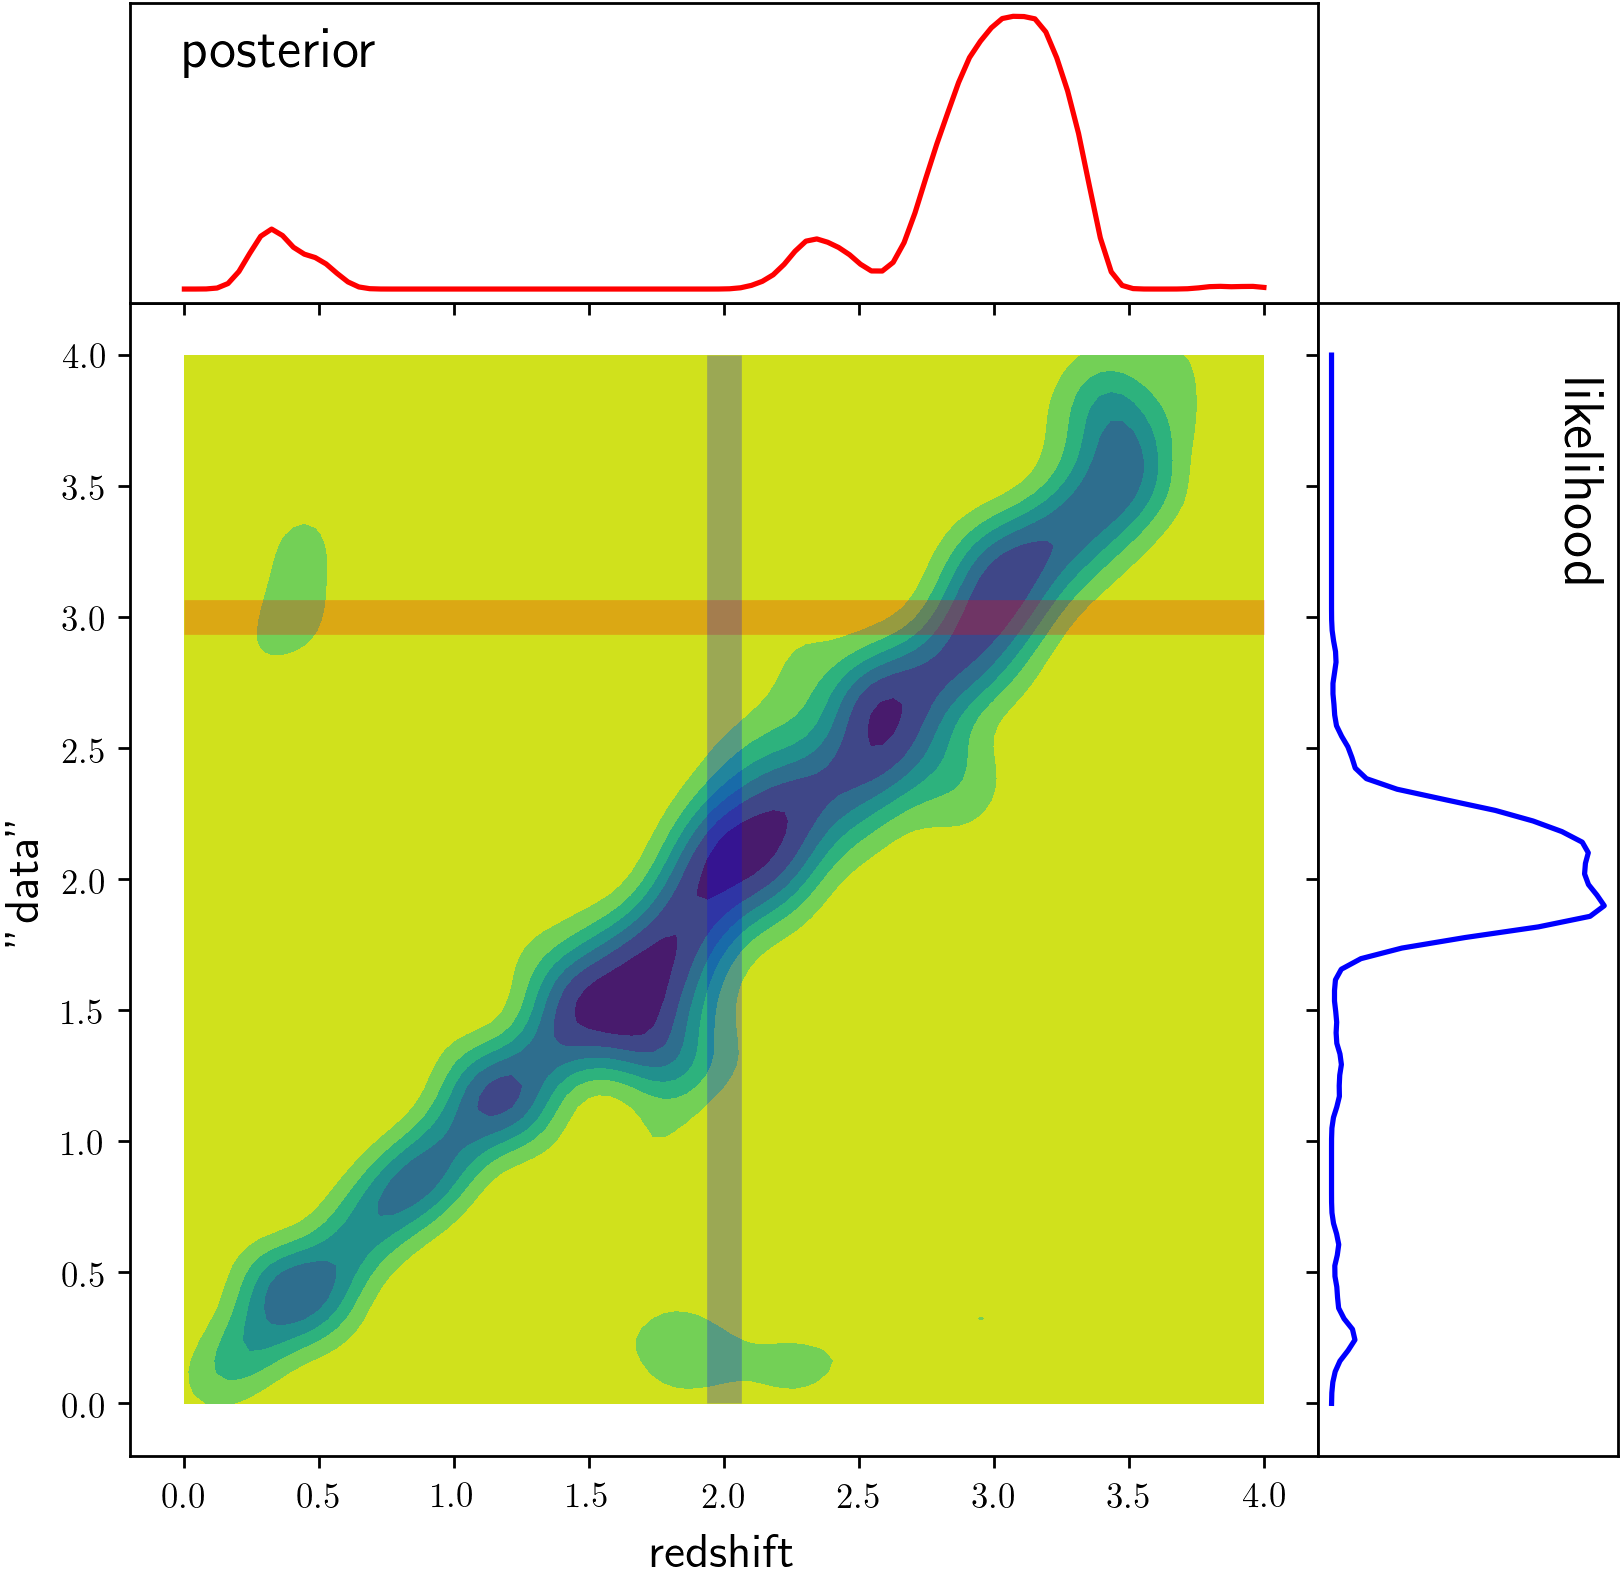
\includegraphics[width=0.74\textwidth]{figures/chippr/jain05.png}
		\caption{
			A generic probability space of redshift (x-axis) and data (y-axis), projected into a single dimension, with vertical cuts and marginals (cyan) indicating the construction of likelihoods and horizontal cuts and marginals (magenta) indicating the construction of posteriors.
			The data (black points) used to generate the contours were extracted from \citet{jain_whole_2015} using WebPlotDigitizer \citep{rohatgi_webplotdigitizer_2019}, with the ideal redshift estimation provided for reference (red line).
			\aim{Choose better colors?}
		}
		\figlabel{fig:pedagogical_scatter}
	\end{center}
\end{figure*}

This description of the physical system corresponds to a forward model by which we actually believe photometry is generated:
\begin{enumerate}
	\item There exists a redshift distribution \nz\ with parameters $\ndphi$.
	\item Galaxy redshifts $\{z_{j}\}$ are independent draws from $\pr{z \gvn \ndphi}$.
	\item Galaxy photometry $\data_{j}$ is drawn from the likelihoods $\pr{\data_{j} \gvn z}$.
\end{enumerate}

\subsection{Probabilistic Model}
\sectlabel{sec:prob}

A forward model such as that of \Sect{sec:forward} corresponds to a probabilistic graphical model (PGM), represented by a directed acyclic graph (DAG) as in \Fig{fig:pgm}.
A DAG conveys the causal relationships between physical parameters and, like a Feynman diagram in the context of particle physics, is a shorthand for mathematical relationships between variables.
The photometric data $\data_{j}$ of a galaxy is drawn from some function of its redshift $z_{j}$, independent of other galaxies' data and redshift.
Both data and redshift are random variables, but data is the one that we observe and redshift is not directly observable.
In this problem, we don't care about further constraining the redshifts of individual galaxies, only the redshift distribution, so we consider redshift to be a \textit{latent variable}.
Because the parameters $\ndphi$ that we seek are causally separated from the data by the latent variable of redshift, we call them \textit{hyperparameters}.
\aim{I'm not explaining the distinction between hyperparameters and parameters adequately.}

\begin{figure}
	\begin{center}
		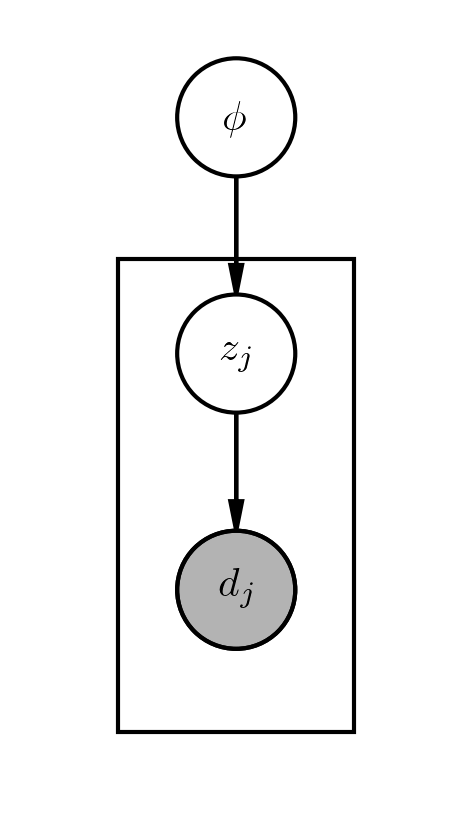
\includegraphics[width=0.2\textwidth]{figures/chippr/pgm.png}
		\caption{The directed acyclic graph of the CHIPPR model, where circles indicate random variables and arrows indicate causal relationships.
			The redshift distribution function parameterized by hyperparameters $\ndphi$ exists independent of the survey of $J$ galaxies, indicated as a box.  
			The redshifts $\{z_{j}\}$ of all galaxies in the survey are latent variables independently drawn from the redshift distribution, which is a function of $\ndphi$. 
			The photometric data $\data_{j}$ for each galaxy is drawn from a function of its redshift $z_{j}$ and observed, indicated by a shaded circle.}
		\figlabel{fig:pgm}
	\end{center}
\end{figure}

The problem facing cosmologists is to determine the true value of $\ndphi$ from observing the photometry $\{\data_{j}\}$ of a large sample of $J$ galaxies $j$.
To self-consistently propagate the uncertainty in the redshifts, however, it is more appropriate to estimate the posterior $\pr{\ndphi \gvn \{\data_{j}\}}$ over all possible values of $\ndphi$ conditioned on all the observed data $\{\data_{j}\}$ available in a generic catalog.
In order to use the DAG of \Fig{fig:pgm} to derive an expression for $\pr{\ndphi \gvn \{\data_{j}\}}$ in terms of \pzpdf s, we must introduce two more concepts, confusingly named the implicit prior and the prior probability density.

When we constrain the redshift of a galaxy using its observed photometric data $\data_{j}$, we are effectively estimating a posterior $\pr{z \gvn \data_{j}}$.
However, to do this, we must have a model for the general relationship between redshifts and photometry, whether empirical, as is the case for machine learning \pzpdf\ methods, or analytic, as is the case for template-based \pzpdf\ methods.
Such a relationship is defined in the space of probability density over redshift, so it must be able to be parameterized by the same functional form $f(z; \ndphi)$ as \nz .
It is thus natural to write it as $\pr{z \gvn \ndphi^{*}}$, where $\ndphi^{*}$ is the parameters for this relationship under some generic \pzpdf\ method.
We call $\pr{z \gvn \ndphi^{*}}$ the \textit{implicit prior}, as it is rarely explicitly known nor chosen by the researcher; for template-based methods where it can be chosen to be ``realistic,'' it may be appropriate to call it an \textit{interim prior}.
Because the implicit prior is unavoidable, the \pzpdf s reported by any method are really \textit{implicit-weighted posteriors} $\pr{z \gvn \data, \ndphi^{*}}$.

%Posteriors differ from likelihoods by way of a prior distribution, so we cannot simply assume that the available data products are \pz\ posteriors $\pr{z \gvn \data_{j}}$.  
%Rather, we have a catalog of implicit-prior weighted \pz\ posteriors $\pr{z \gvn \data_{j}, \ndphi^{*}}$.  
%There must have been some interim prior probability distribution $p(z|\vec{\theta}^{*})$ defined in terms of the interim prior parameter values (hereafter the interim prior) $\vec{\theta}^{*}$ explicitly chosen or implicitly made to perform the calculation of the probabilistic photo-$z$s.  
%If it is implicit, it may not be representable in the parametrization we have chosen, and furthermore it may not be known at all; a method that produces interim photo-$z$ posteriors of this kind is not suitable for inference.  
%However, so long as the implicit prior is known, hierarchical inference is possible. 

The implicit prior $\ndphi^{*}$ may be thought of as an initial guess for the parameters contained in $\ndphi$, inspired by the generative model for photometry from the redshift distribution functions and including some parameters defining intrinsic galaxy spectra and instrumental effects. 
(See \citealt{Benitez2000} for more detail.)  
For statistical purposes, we would like any interim prior to be uninformative, but this is rarely achievable.  
In the case of estimating \nz\ photometrically, it is common to use $\ndphi^{*}$ corresponding to \nz\ derived from some different, spectroscopically confirmed sample or from a cosmological simulation.

The prior probability density $\pr{\ndphi}$ is a more familiar concept in astronomy; to progress, we will have to choose a prior probability density over all possible parameters $\ndphi$.
This prior need not be excessively proscriptive; for example, it may be chosen to enforce smoothness at physically motivated scales in redshift without imposing any particular region as over- or under-dense.

With these definitions, we obtain the desired expression for $\pr{\ndphi \gvn \{\data_{j}\}}$,
\begin{align}
\begin{split}
\eqlabel{eqn:fullpost}
\pr{\ndphi \gvn \{\data_{j}\}} & \propto \pr{\ndphi}\left[\integral{\prod_{j=1}^{J} \left(\pr{z \gvn \data_{j}, \ndphi^{*}}\pr{z \gvn \ndphi}(\pr{z \gvn \ndphi^{*}})^{-1}\right)}{z}\right] ,
\end{split}
\end{align}
the heart of \Chippr.
The derivation is provided below in \Sect{app:math}.

\subsubsection{Derivation}
\sectlabel{app:math}

%We begin by parametrizing $N(z)$ in terms of $\vec{\theta}$, comprising some set of hyperparameters that define the form $N(z)$ may take in whatever basis we choose.  
%We define a function $f_{\vec{\theta}}(z)=N(z)$ that transforms these hyperparameters into the redshift distribution function $N(z)$.  
%Because 
%\begin{equation}
%\eqlabel{eq:definition}
%N(z) \propto p(z \gvn \vec{\theta}),
%\end{equation}
%we may discontinue discussion of $N(z)$ in favor of the likelihood $p(z|\vec{\theta})$.

In this \paper, we work exclusively with log-probabilities.  
What we wish to estimate is then the full log-posterior probability distribution (hereafter the full log-posterior) of the hyperparameters $\ndphi$ given the catalog of photometry $\{\data_{j}\}$.

By Bayes' Rule, the full log-posterior
\begin{equation}
\eqlabel{eqn:basicbayes}
\ln[\pr{\ndphi \gvn \{\data_{j}\}}] = \ln[\pr{\{\data_{j}\} \gvn \ndphi}] + \ln[\pr{\ndphi}] - \ln[\pr{\{\data_{j}\}}]
\end{equation}
may be expressed in terms of the full log-likelihood probability distribution (hereafter the full log-likelihood) $\ln[\pr{\{\data_{j}\} \gvn \ndphi}]$ by way of a hyperprior log-probability distribution (hereafter the hyperprior) $\ln[\pr{\ndphi}]$ over the hyperparameters and the log-evidence probability of the data $\ln[\pr{\{\data_{j}\}}]$.
However, the evidence is rarely known, so we probe the full log-posterior modulo an unknown constant of proportionality.

The full log-likelihood may be expanded in terms of a marginalization over the redshifts as parameters, as in 
\begin{equation}
\eqlabel{eqn:marginalize}
\ln[\pr{\{\data_{j}\} \gvn \ndphi}] = \ln\left[\integral{\pr{\{\data_{j}\} \gvn \{z_{j}\}} \pr{\{z_{j}\} \gvn \ndphi}}{\{z_{j}\}}\right].
\end{equation}

We shall make two assumptions of independence in order to make the problem tractable; their limitations are be discussed below.  
First, we take $\ln[\pr{\{\data_{j}\} \gvn \{z_{j}\}}]$ to be the sum of $J$ individual log-likelihood distribution functions $\ln[\pr{\data_{j} \gvn z_{j}}]$, as in 
\begin{equation}
\eqlabel{eqn:indiedat}
\ln[\pr{\{\data_{j}\} \gvn \{z_{j}\}}] = \sum_{j=1}^{J}\ \ln[\pr{\data_{j} \gvn z_{j}}],
\end{equation}
a result of the definition of probabilistic independence encoded by the box in \Fig{fig:pgm}.
Second, we shall assume the true redshifts $\{z_{j}\}$ are $J$ independent draws from the true $\pr{z \gvn \ndphi}$.  
Additionally, $J$ itself is a Poisson random variable.  
The combination of these assumptions is given by 
\begin{equation}
\eqlabel{eqn:indie}
\ln[\pr{\{z_{j}\} \gvn \ndphi}] = -\integral{f(z; \ndphi)}{z} + \sum_{j=1}^{J}\ \ln[\pr{z_{j} \gvn \ndphi}].
\end{equation}
%It is important to note that the integral $\integral{n(z)}{z} N(z)\ dz$ is not constrained to equal the variable defining the Poisson distribution but instead $J$ by \Eq{eq:definition}, which can be thought of as another parameter.  
The derivation differs when $J$ is not known, say, when we want to learn about a distribution in nature rather than a distribution specific to data in hand, but for a photometric galaxy catalog where the desired quantity is $n(z)$ for the galaxies entering a larger cosmology calculation, it is a fixed quantity.
A detailed discussion of this matter may be found in \citet{Foreman-Mackey2014}.  
Applying Bayes' Rule, we may combine terms to obtain 
\begin{equation}
\eqlabel{eqn:posterior}
\ln[\pr{\ndphi \gvn \{\data_{j}\}}] \propto \ln[\pr{\ndphi}] - \integral{f(z; \ndphi)}{z} + \sum_{j=1}^{J}\ln\left[\integral{\pr{\data_{j} \gvn z} \pr{z \gvn \ndphi}}{z}\right].
\end{equation}

%\Eq{eq:posterior} contains two quantities that merit further discussion, the prior distribution $p(\vec{\theta})$ discussed further in \Sect{sec:exp} and the photo-$z$ log-likelihoods $\ln[p(\vec{d}_{j}|z_{j})]$ that have not been mentioned since \Eq{eq:marginalize}.  
%Though photo-$z$ log-likelihoods would be desirable for use in these equations, they are not generally the product of either empirical and data-driven methods for obtaining photo-$z$ probability distributions.  
%Though probabilistic photo-$z$s are typically reported as generic probability distributions $p(z_{j})$, the methods that produce them may be understood to always yield posteriors, probability distributions conditioned on the data we believe to be true.  
%If they were not based in this assumption, they would require a sum over an infinite space of possible datasets.

Since we only have access to implicit \pz\ posteriors, we must be able to write the full log-posterior in terms of implicit \pz\ log-posteriors rather than the log-likelihoods of \Eq{eqn:posterior}.
To do so, we will need an explicit statement of this implicit prior $\ndphi^{*}$ for whatever method is chosen to produce the implicit \pz\ posteriors.  

To perform the necessary transformation from likelihoods to posteriors, we follow the reasoning of \citet{Foreman-Mackey2014}.  
Let us consider the probability of the parameters conditioned on the data and an interim prior and rewrite the problematic likelihood of \Eq{eqn:posterior} as 
\begin{equation}
\eqlabel{eqn:trick}
\ln[\pr{\data_{j} \gvn z}] = \ln[\pr{\data_{j} \gvn z}] + \ln[\pr{z \gvn \data_{j}, \ndphi^{*}}] - \ln[\pr{z \gvn \data_{j}, \ndphi^{*}}].
\end{equation}

Once the implicit prior $\ndphi^{*}$ is explicitly introduced, we may expand the last term in \Eq{eqn:trick} according to Bayes' Rule to get 
\begin{equation}
\eqlabel{eqn:expand}
\ln[\pr{\data_{j} \gvn z}] = \ln[\pr{\data_{j} \gvn z}] + \ln[\pr{z \gvn \data_{j}, \ndphi^{*}}] + \ln[\pr{\data_{j} \gvn \ndphi^{*}}] - \ln[\pr{z \gvn \ndphi^{*}}] - \ln[\pr{\data_{j} \gvn z, \ndphi^{*}}].
\end{equation}
Because there is no direct dependence of the data upon the hyperparameters, we may again expand the term $\ln[\pr{\data_{j} \gvn z, \ndphi^{*}}]$ to obtain 
\begin{equation}
\eqlabel{eqn:indterm}
\ln[\pr{\vec{d}_{j} \gvn z}] = \ln[\pr{\data_{j} \gvn z}] + \ln[\pr{z \gvn \data_{j}, \ndphi^{*}}] + \ln[\pr{\data_{j} \gvn \ndphi^{*}}] - \ln[\pr{z \gvn \ndphi^{*}}] - \ln[\pr{\data_{j} \gvn z}] - \ln[\pr{\data_{j} \gvn \ndphi^{*}}].
\end{equation}
Canceling the undesirable terms for the inaccessible likelihood $\ln[\pr{\data_{j} \gvn z}]$ and trivial $\ln[\pr{\data_{j} \gvn \ndphi^{*}}]$ yields
\begin{equation}
\eqlabel{eqn:cancel}
\ln[\pr{\data_{j} \gvn z}] = \ln[\pr{z \gvn \data_{j}, \ndphi^{*}}]  - \ln[\pr{z \gvn \ndphi^{*}}].
\end{equation}
We put this all together to get the full log-posterior probability distribution of 
\begin{equation}
\eqlabel{eqn:final}
\ln[\pr{\ndphi \gvn \{\data_{j}\}}] \propto \ln[\pr{\ndphi}] + \ln \left[\integral{\exp \left[\sum_{j=1}^{J} \left(\ln[\pr{z \gvn \data_{j}, \ndphi^{*}}] + \ln[\pr{z \gvn \ndphi}] - \ln[\pr{z \gvn \ndphi^{*}}]\right)\right]}{z}\right] ,
\end{equation}

The argument of the integral in the log-posterior of \Eq{eqn:final} depends solely on knowable quantities (and those we must explicitly assume) and can be calculated for a given sample of \pz\ log-posteriors $\{\ln[\pr{z \gvn \data_{j}, \ndphi^{*}}]\}$ and the implicit prior $\pr{z \gvn \ndphi^{*}}$ with which they were obtained, noting the relation of 
\begin{equation}
\eqlabel{eqn:params}
\pr{z \gvn \ndphi} = \frac{f(z; \ndphi)}{\integral{f(z; \ndphi)}{z}}.
\end{equation}
Since we cannot know constant of proportionality, we sample the desired full log-posterior $\ln[\pr{\ndphi \gvn \{\data_{j}\}}]$ using Monte Carlo-Markov chain (MCMC) methods.  
The method outlined here is valid regardless of how the implicit \pz\ log-posteriors are obtained so the many approaches to producing \pzpdf s will not be rehashed; though the matter is outside the scope of this \paper, reviews of various methods have been presented in the literature \citep{Sheldon2012, Ball2008, CarrascoKind2013, CarrascoKind2014a}, and will be briefly reviewed in \Chap{pzdc1}.
%
%\begin{align}
%\begin{split}
%\eqlabel{eqn:fullpost}
%\ln[\pr{\ndphi \gvn \{\data_{j}\}}] & \propto \ln[\pr{\ndphi}] + \ln \left[\integral{\exp \left[\sum_{j=1}^{J} \left(\ln[\pr{z \gvn \data_{j}, \ndphi^{*}}] + \ln[\pr{z \gvn \ndphi}] - \ln[\pr{z \gvn \ndphi^{*}}]\right)\right]}{z}\right] ,
%\end{split}
%\end{align}

\subsubsection{Model Limitations}
\sectlabel{sec:limitations}

Finally, we explicitly review the assumptions made by this approach, which are as follows:

\begin{enumerate}
	\item Photometric measurements of galaxies are statistically independent Poisson draws from the set of all galaxies such that \Eq{eqn:indiedat} and \Eq{eqn:indie} hold.
	\item We take the reported \pzip s to be accurate, free of model misspecification; draws thereof must not be inconsistent with the distribution of photometry and redshifts.
	Furthermore, we must be given the implicit prior $\ndphi^{*}$ used to produce the \pzip s.
	\item We must assume a hyperprior distribution $\pr{\ndphi}$ constraining the underlying probability distribution of the hyperparameters, which is informed by our prior beliefs about the true redshift distribution function.
\end{enumerate}

These assumptions have known limitations.  
First, the photometric data are not a set of independent measurements; the data are correlated not only by the conditions of the experiment under which they were observed (instrument and observing conditions) but also by redshift covariances resulting from physical processes governing underlying galaxy spectra and their relation to the redshift distribution function.
Second, the reported \pzip s may not be trustworthy; there is not yet agreement on the best technique to obtain \pzpdf s, and the implicit prior may not be appropriate or even known to us as consumers of \pzip s.  
Third, the hyperprior may be quite arbitrary and poorly motivated if the underlying physics is complex, and it can only be appropriate if our prior beliefs about \nz\ are accurate.

%\clearpage
\subsection{Implementation}
\sectlabel{sec:exp}

I implemented the \Chippr\ model in code in order to perform tests of its validity and to compare its performance to that of traditional alternatives.
In \Sect{sec:mcmc}, I describe the publicly available \chippr\ library.
In \Sect{sec:acorr}, I outline how \chippr\ can be used to sample the full log-posterior distribution $\ln[\pr{\ndphi \gvn \{\data_{j}\}}]$.

%\clearpage
\subsubsection{Code}
\sectlabel{sec:mcmc}

\chippr\ is a \python\ 2 library that includes an implementation of the \Chippr\ model as well as an extensive suite of tools for comparing \Chippr\ to other approaches.
\aim{Cite GitHub here.}

Though there are plans for future expansion to more flexible parameterizations, the current version of \chippr\ uses a log-space piecewise constant parameterization
\begin{equation}
\eqlabel{eqn:logstepfunc}
f(z; \ndphi) = \exp[\phi^{k}]\ \mathrm{if}\ z^{k} < z < z^{k+1}
\end{equation}
for \nz\ and every \pzpdf, satisfying
\begin{equation}
\eqlabel{eqn:logstepfuncnorm}
\sum_{k=1}^{K} \exp[\phi^{k}] \delta z^{k} = 1
\end{equation}
with $K$ bins of width $\delta z^{1}, \dots, \delta z^{K}$ defined by endpoints $z^{0}, \dots, z^{K}$.
\aim{Maybe include an equation for a general piecewise constant function here (which is currently in \Chap{qp})?}
Thus each $\pr{z \gvn \data_{j}} = f(z; \ndphi_{j})$ has parameters $\ndphi_{j}$ that are defined in the same basis as those of \nz.
To infer the full log-posterior distribution $\ln[\pr{\ndphi \gvn \{\data_{j}\}}]$, one must provide a plaintext file with $K+1$ redshift bin endpoints $\{z_{k}\}$, the parameters $\ndphi^{*}$ of the implicit log-prior, and the parameters $\{\ndphi_{j}\}$ of the log-posteriors $\ln[\pr{z \gvn \data_{j}, \ndphi^{*})}$.

The \emcee \citep{Foreman-Mackey2013} implementation of ensemble sampling is used to sample the full log-posterior of \Eq{eqn:final}. 
\chippr\ accepts a configuration file of user-specified parameters, among them the number $W$ of walkers.
At each iteration $i$ and for each walker, a proposal distribution $\hat{\ndphi}_{i}$ is drawn from the log-prior distribution and evaluated for acceptance to or rejection from the full log-posterior distribution.

Two threshold conditions are defined, one designating all previous samples to be ignored as as products of a burn-in phase and another indicating when a sufficient number of post-burn samples have been accepted.  
In this case, the first threshold (described in \Sect{sec:acorr}) is defined in terms of sub-runs of $10^{3}$ accepted samples, and the second is defined as an accumulation of $10^{4}$ samples.

Though previous versions used \texttt{HDF5} for the primary I/O format due to its efficiency for large quantities of data, it was abandoned in favor of \texttt{pickle} in the working release due to the instability of the \python\ implementation of the format on high-performance computing systems.  
The resulting output is a set of $I$ ordered \texttt{hickle} files enumerated by $\rho$ containing the state information after each sub-run.  
The state information includes $\frac{I_{0}}{s}$ actual samples $\ndphi_{i}$ for a pre-specified chain thinning factor $s$ and their full posterior probabilities $\pr{\ndphi_{i} \gvn \{\data_{j}\}}$ as well as the autocorrelation times and acceptance fractions calculated for each element of $\ndphi$ over the entire sub-run.  

%\clearpage
\subsubsection{Convergence Criteria}
\sectlabel{sec:acorr}

In addition to qualitative visual inspection of the chains, two quantities that probe the convergence of the sampler are used in this study, the autocorrelation time and the Gelman-Rubin convergence criterion.  
%\Fig{fig:chains} shows the %evolution of the values of one parameter of one walker over the course of all %iterations of the sampler.

%\begin{figure}
%%\includegraphics[width=0.5\textwidth]{figs/null/chain0.pdf}
%\caption{This figure shows the evolution of one walker's parameter values for 
%one element of the parameter vector $\vec{\theta}$ as a function of iteration 
%number, demonstrating the completion of the burn-in phase.}
%\label{fig:chains}
%\end{figure}

The autocorrelation time is effectively a measure of the efficiency of the method and can be described as the expected number of iterations necessary to accept a new sample independent of the current accepted sample.  
A sampler that converges faster will have a smaller autocorrelation time, and smaller autocorrelation times are preferable because it means fewer iterations are wasted on non-independent samples when independent samples are desired.  
See \citet{Foreman-Mackey2013} for a more complete exploration of the autocorrelation time.  
In all tests discussed here, autocorrelation times across walkers and parameters were approximately 20, meaning two samples 20 or more iterations apart were independent, a satisfactory level of efficiency.  
Low autocorrelation times are a necessary but not always sufficient convergence condition, as the autocorrelation times calculated for tests in this paper were constant across all sub-runs, even those that were obviously burning in.  

The Gelman-Rubin statistic
\begin{equation}
\eqlabel{eqn:gr}
R_{k} = \sqrt{\frac{(1 - \frac{2}{I_{0}}) w_{k} + \frac{2}{I_{0}} b_{k}}{w_{k}}},
\end{equation}
a weighted sum of the mean $w_{k}$ of the variances within individual walkers' chains and the variance $b_{k}$ between chains of different walkers $m$, is calculated over each sub-run $i$ to determine the duration of the burn-in period.  
Convergence is achieved when the statistic approaches unity.  

\subsection{Comparison with Alternative Approaches}
\sectlabel{sec:sheldon}

In this study, we compare the results of \Eq{eqn:fullpost} to those of the two most common approaches to estimating \nz\ from a catalog of \pzpdf s: the distribution $n(z_{\mathrm{max}})$ of the redshifts at maximum posterior probability
\begin{equation}
\eqlabel{eqn:mmap}
f^{MMAP}(z; \hat{\ndphi}) = \sum_{j=1}^{J}\ \delta(z, \mathrm{mode}[\pr{z \gvn \data_{j}, \ndphi^{*}}])
\end{equation}
(i.e. the distribution of modes of the \pzpdf s) and the stacked estimator of \Eq{eqn:stacked}, which can be rewritten as 
\begin{equation}
\eqlabel{eqn:stacked}
f^{stack}(z; \hat{\ndphi}) = \sum_{j=1}^{J}\ \pr{z \gvn \data_{j}, \ndphi^{*}}
\end{equation}
in terms of the implicit \pz\ posteriors we have.
These two approaches have been compared to one another by \citet{Hildebrandt2012}, \citet{Benjamin2013}, and \citet{Asorey2016} in the past but not to \Chippr.

Point estimation converts the interim photo-$z$ posteriors $\pr{z \gvn \data_{j}, \ndphi^{*}}$ into delta functions with all probability at a single estimated redshift.  
Some variants of point estimation choose this single redshift to be that of maximum a posteriori probability $\mathrm{mode}[\pr{z \gvn \data_{j}, \ndphi^{*}}]$ or the expected value of redshift $\langle z \rangle = \integral{z \pr{z \gvn \data_{j}, \ndphi^{*}}}{z}$.
\cite{tanaka_photometric_2018} directs attention to deriving an optimal point estimate reduction of a \pzpdf, but since the purpose of this \paper is to compare against the most established alternative estimators of \nz, its use will be postponed until a future study.
Stacking these modified \pzpdf s leads to the marginalized maximum a posteriori (MMAP) estimator and the marginalized expected value (MExp) estimator, though only the former is included in this study since the latter has fallen out of favor in recent years.

It is worth discussing the relationship between point estimation and stacking.  
When the point estimator of redshift is equal to the true redshift, stacking delta function \pzpdf s will indeed lead to an accurate recovery of the true redshift distribution function.  
However, stacking is in general applied indiscriminately to broader \pzpdf s and imperfect point estimators of redshift.  
It is for these reasons that alternatives are considered here.

A final estimator of the hyperparameters is the maximum marginalized likelihood estimator (MMLE), the value of $\ndphi$ maximizing the log posterior given by \Eq{eqn:final} using any optimization code.  
To compare with sampling, the MMLE also depends on the choice of the hyperprior distribution, and it does not produce a full posterior probability distribution over the parameters of interest, only point estimators.  
It must be noted that computation of the MMLE may be unstable depending on the strengths and weaknesses of the optimizer.  
In general, derivatives will not be available for the full posterior distribution, restricting optimization methods used.
%\begin{equation}
%\label{eq:mmle}
%\ln[p(\{\vec{d}_{j}\}|\vec{\theta})] \propto -\int\ f_{\vec{\theta}}(z)\ 
%dz+\sum_{j=1}^{J}\ln\left[\int\ 
%\exp\left[\ln[p(z_{j}|\vec{d}_{j},\vec{\theta}^{*})]+\ln[f_{\vec{\theta}}(z)]-\l
%n[f_{\vec{\theta}^{*}}(z)]\right]\ dz\right],
%\end{equation}
%accessible with any optimization code.

In \Sect{sec:diag} we outline the measures used to evaluate the performance of the method.

%\clearpage
\subsubsection{Comparison metrics}
\sectlabel{sec:diag}

The results of the computation described in \Sect{sec:mcmc} are evaluated for accuracy on the basis of some quantitative measures.  
Beyond visual inspection of samples, we calculate summary statistics to quantitatively compare different estimators' precision and accuracy.  
Since MCMC samples of hyperparameters are Gaussian distributions, we can quantify the breadth of the distribution for each hyperparameter using the standard deviation regardless of whether the true values are known.  

In simulated cases where the true parameter values are known, we calculate the Kullback-Leibler divergence (KLD), given by 
\begin{equation}
\eqlabel{eqn:kl}
KL_{',\ddagger} = \integral{\pr{z \gvn \ndphi'} \ln \left[ \frac{\pr{z \gvn \ndphi'}}{\pr{z \gvn \ndphi^{\dagger}}} \right]}{z} ,
\end{equation}
which measures a distance from parameter values $\ndphi'$ to true parameter values $\ndphi^{\dagger}$, which is invariant under changes of variables.  
We note that $KL_{',\dagger} \neq KL_{\dagger,'}$ and is only interpretable when there is a notion that $\ndphi^{\dagger}$ is closer to the truth than $\ndphi'$.
In simulated tests, $\ndphi^{\dagger}$ is the true value and $\ndphi'$ is that produced by one of the methods in question.

\section{Validation}
\sectlabel{sec:alldata}

We compare the results of \Chippr\ to those of stacking and the histogram of \pzpdf\ maxima (modes) on mock data in the form of catalogs of emulated \pzpdf s generated via the forward model discussed in \Sect{sec:forward}.
\Fig{fig:flowchart} illustrates the implementation of this forward model used in this \paper.

\begin{figure*}
	\begin{center}
		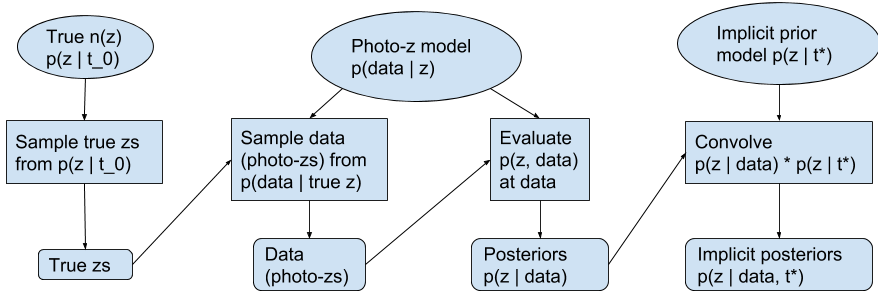
\includegraphics[width=\textwidth]{figures/chippr/flowchart.png}
		\caption{A flow chart illustrating the forward model used to generate mock data in the validation of \Chippr, as described in \Sect{sec:forward}.
		Ovals indicate a quantity I choose in order to generate the data, rectangles indicate an operation I perform, and rounded rectangles indicate a quantity created by the forward model.
		Arrows indicate the inputs and outputs of each operation performed to simulate mock \pzpdf\ catalogs.}
		\figlabel{fig:flowchart}
	\end{center}
\end{figure*}

The true redshift distribution used in these tests is a particular instance of the gamma function
\begin{equation}
\eqlabel{eqn:gamma}
n^{\dagger}(z) = \frac{1}{2 c_{z}} \left(\frac{z}{c_{z}}\right)^{2}\ \exp\left[-\frac{z}{c_{z}}\right]
\end{equation}
with $c_{z} = 0.3$, because it has been used in forecasting studies for \des\ and \lsst.
\aim{I learned this from talking to people and don't know of a published source that talks about the nitty gritty of the internal validation tests performed before there was data.}

The mock data emulates the three sources of error of highest concern to the \pz\ community: intrinsic scatter, catastrophic outliers, and systematic bias.
Tests including all three effects at the tolerance levels of \lsst\ (see Table~\ref{intro:tab:tab:lsstsrd}) are presented in \Sect{sec:results}, but \Fig{fig:mega_scatter} illustrates these three effects individually at twice the tolerance of \lsst\ for demonstrative purposes.

\begin{figure}
	\begin{center}
		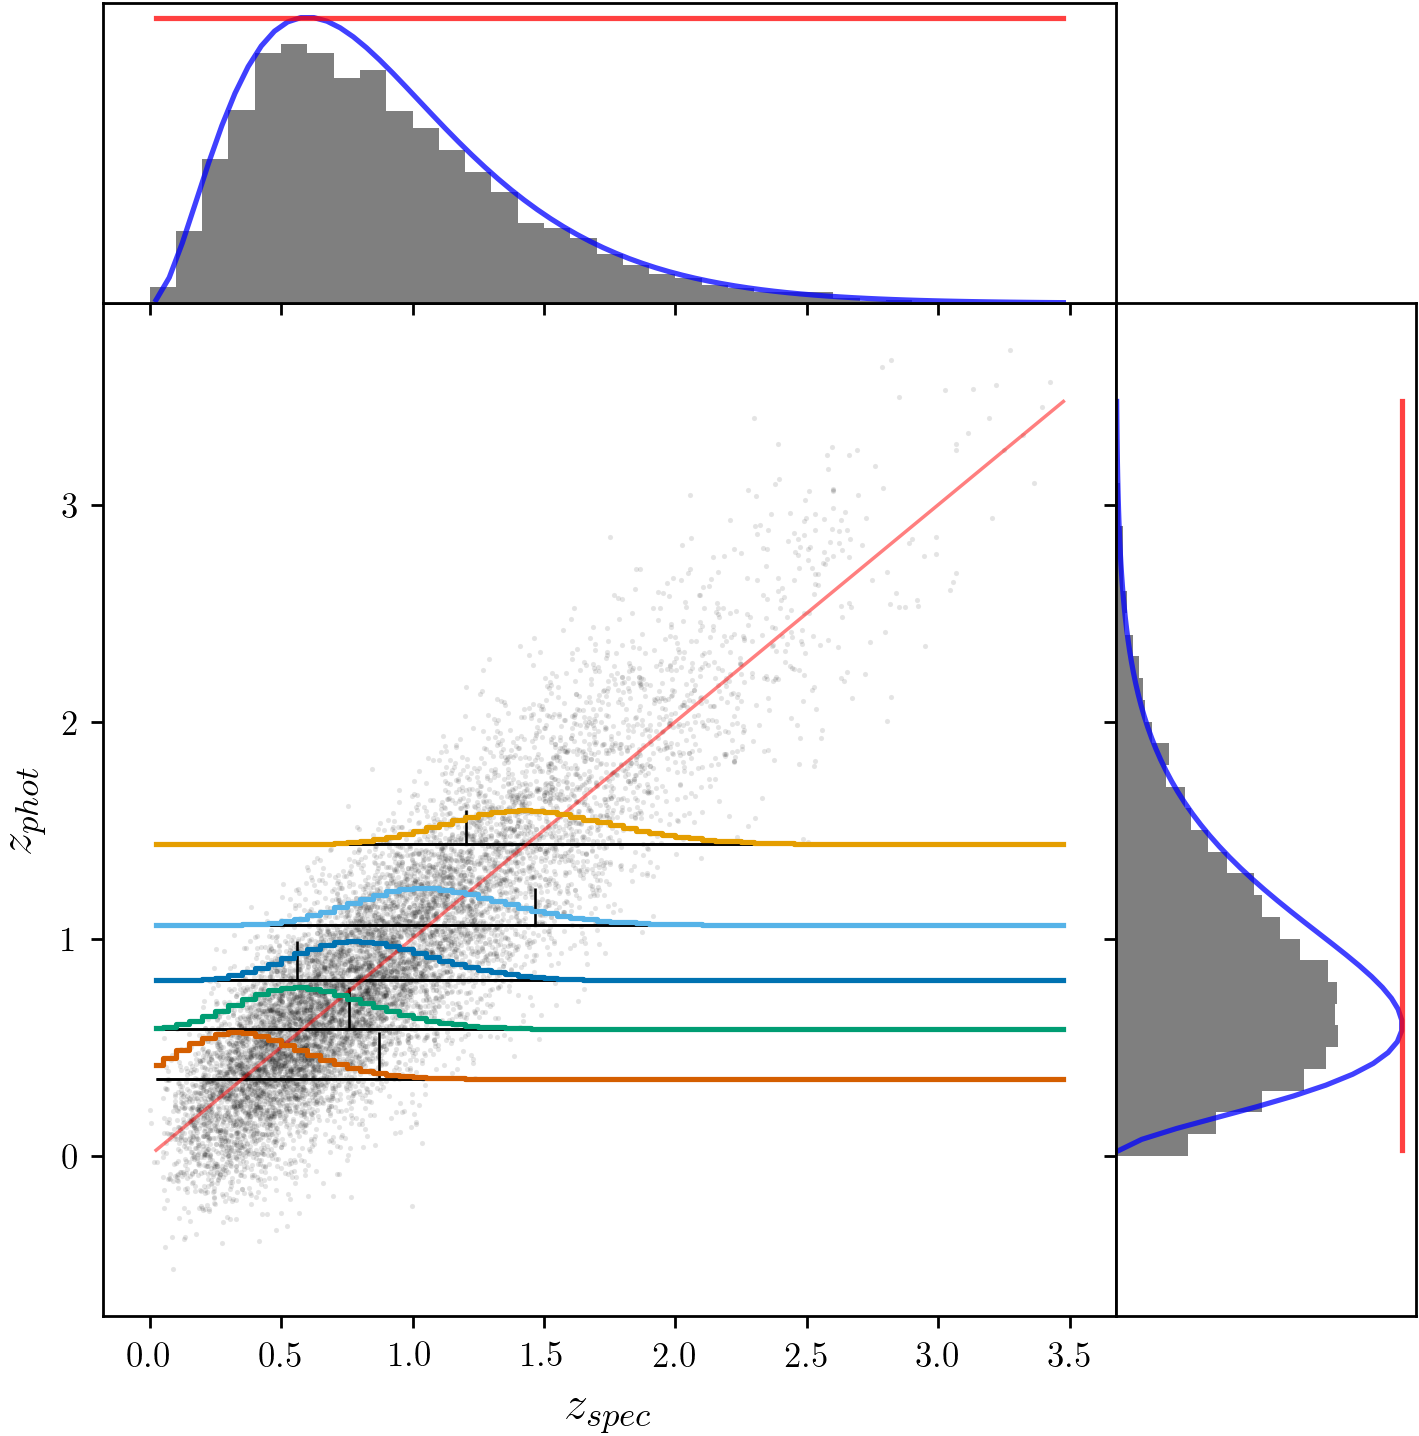
\includegraphics[width=0.24\textwidth]{figures/chippr/scatter_scatplot.png}
		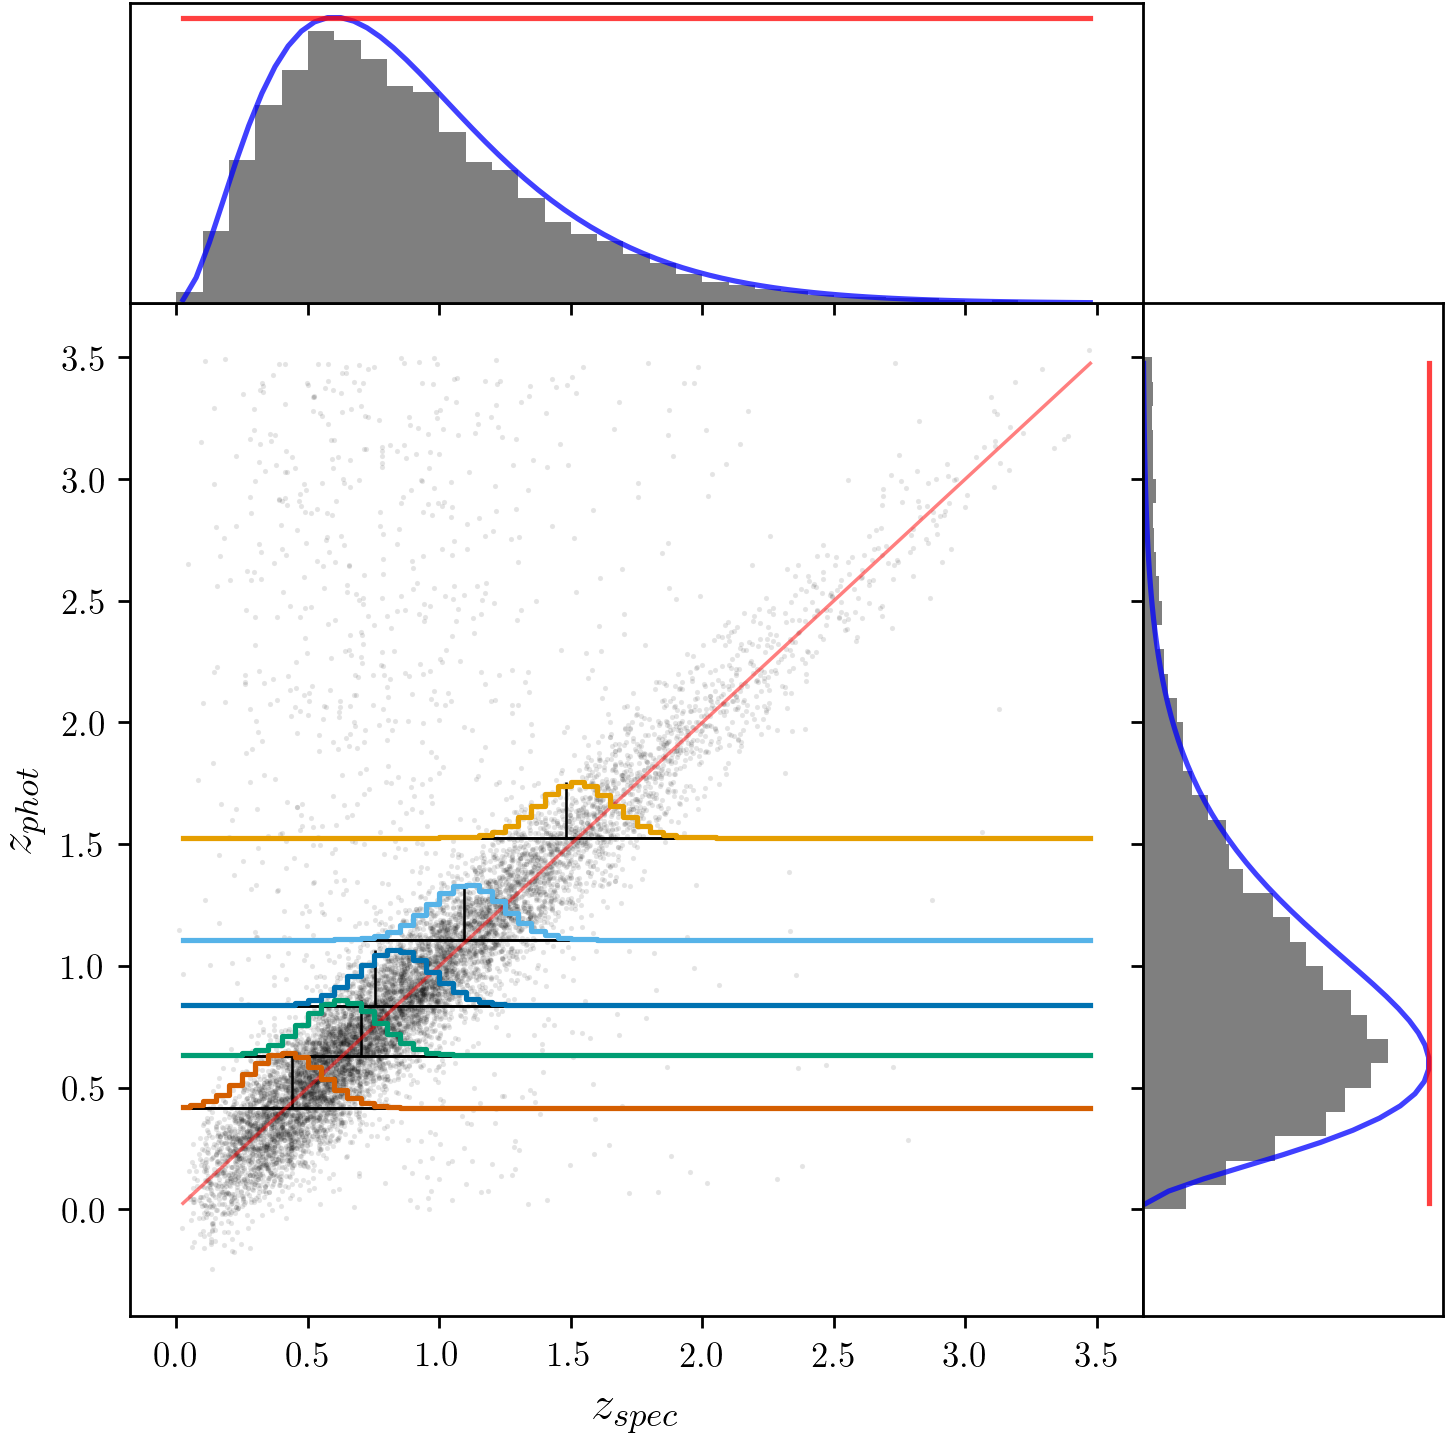
\includegraphics[width=0.24\textwidth]{figures/chippr/outlier_scatplot.png}
		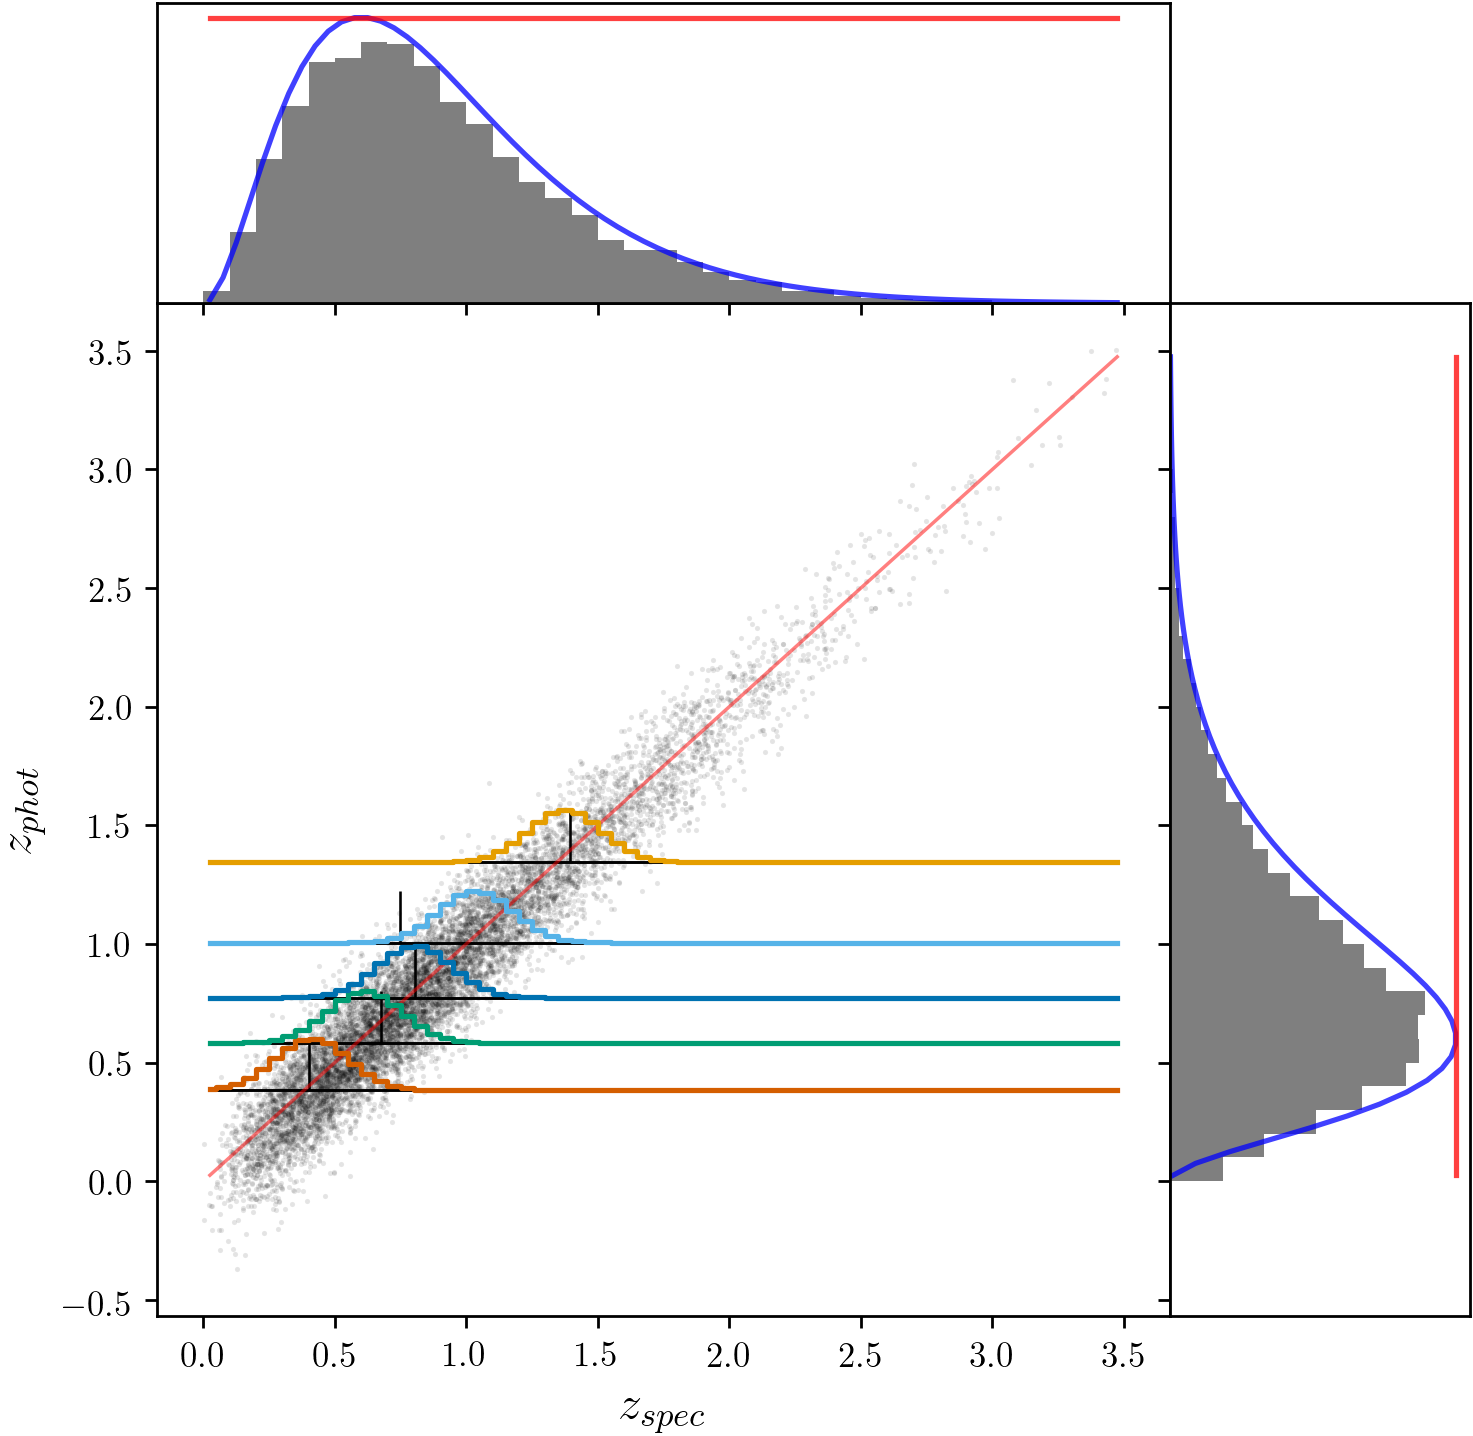
\includegraphics[width=0.24\textwidth]{figures/chippr/bias_scatplot.png}
		\caption{The joint probability space of true and estimated redshift for the three concerning \pz\ systematics: intrinsic scatter (left), uniform outliers (center), and bias (right).
			The points indicate samples in the space of mock data and redshift, akin to the standard scatterplots of true and estimated redshift.
			Colored lines indicate posterior probabilities evaluated at the given estimated redshift.
			The insets show marginal histograms (gray) in each dimension, that can be compared with the true \nz\ used to make the figure (blue curve) to see the effect of the isolated systematic.
		}
		\figlabel{fig:mega_scatter}
	\end{center}
\end{figure}

The hyperprior distribution chosen here is a multivariate normal distribution with mean $\vec{\mu}$ equal to the implicit prior $\ndphi^{*}$ and covariance
\begin{equation}
\eqlabel{eqn:priorcov}
\Sigma_{k,k'} = q\ \exp[-\frac{e}{2}\ (\bar{z}_{k}-\bar{z}_{k'})^{2}]\ +\ t\delta(k,k')
\end{equation}
inspired by one used in Gaussian processes, where $k$ and $k'$ are indices ranging from $1$ to $K$ and $q=1.0$, $e=100.0$, and $t=q\cdot10^{-5}$ are constants chosen to permit draws from this prior distribution to produce shapes similar to that of a true $\tilde{\ndphi}$.  
We adapt the full log-posterior of \Eq{eqn:final} to the chosen binning of redshift space.
%An example of such samples from the prior are shown in \Fig{fig:prior}.
%
%\begin{figure}
%%	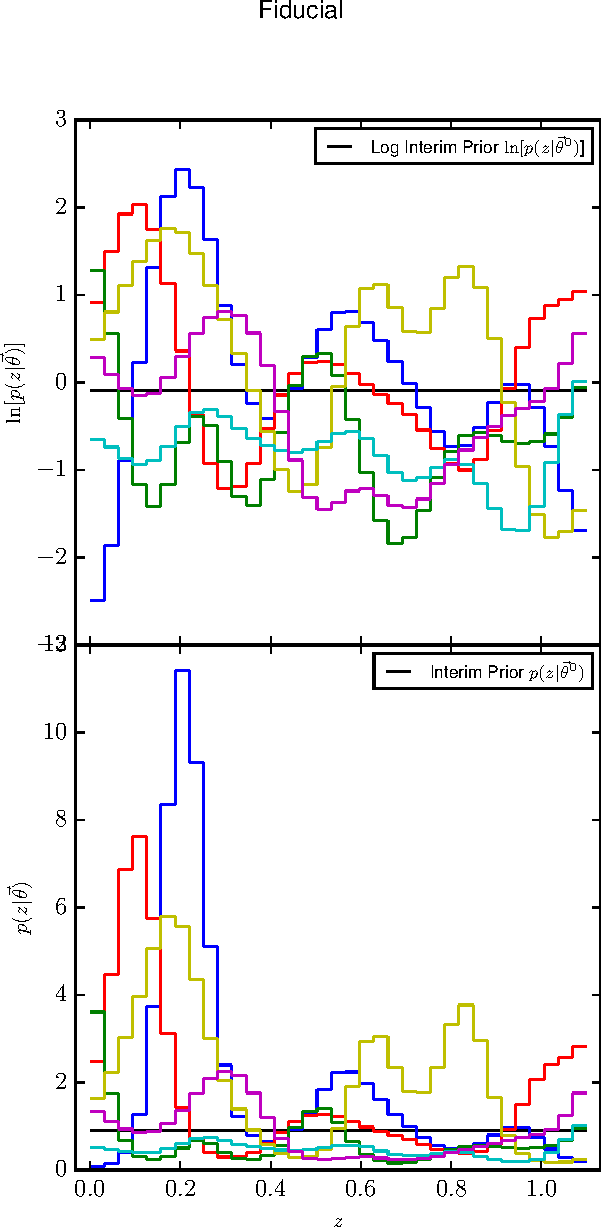
\includegraphics[width=0.5\textwidth]{figures/chippr/null_priorsamps.pdf}
%	\caption{\aim{I need to remake this one because it uses the wrong notation and I stopped making it automatically a while ago.}
%		Samples (colored lines) of $\pr{z \gvn \ndphi}$ where each $\ndphi$ is drawn from the hyperprior distribution $\pr{\ndphi}$ given in \Eq{eqn:priorcov}.}
%	\figlabel{fig:prior}
%\end{figure}

The sampler is initialized with $W=100$ walkers each with a value chosen from a Gaussian distribution of identity covariance around a sample from the hyperprior distribution.  

%\Sect{sec:fake-data} considers a delta function true redshift distribution, but the other sections consider only this physically motivated true \nz.
%\aim{Discuss why it perhaps shouldn't be considered physically motivated -- might not have decided that's what the real thing looks like if we hadn't been stacking all along}

%\subsection{Toy Model}
%\sectlabel{sec:fake-data}
%
%\aim{Commented out but may add back in later.}

%We test the sampler in a case of a highly unrealistic but strongly featured true $N(z)$, that of the lower panel of \Fig{fig:physpz}.  
%This is done to show that the sampler works even in extreme and unanticipated conditions.  
%Instead of sampling the physically motivated true distribution $p(z|\vec{\theta}')$ as in \Sect{sec:mock}, we as

%\Fig{fig:toy-comp} compares the mean of the posterior samples to the results of stacking and marginalized likelihood maximization.  
%It can be seen that the marginalized maximum likelihood estimator is best at recovering the true distribution approaching a delta function due to the nature of the optimizer, which considers each component of the hyperparameter vector to be independent of all others.  
%Other estimators predict a broader distribution than the truth, with stacking broadening it the most and the mean of the samples broadening it the least.  
%Though the sampler does not consider components of the hyperparameter vector to be independent, it is flexible enough to provide good constraints on the true $N(z)$.
%
%\begin{figure}
%	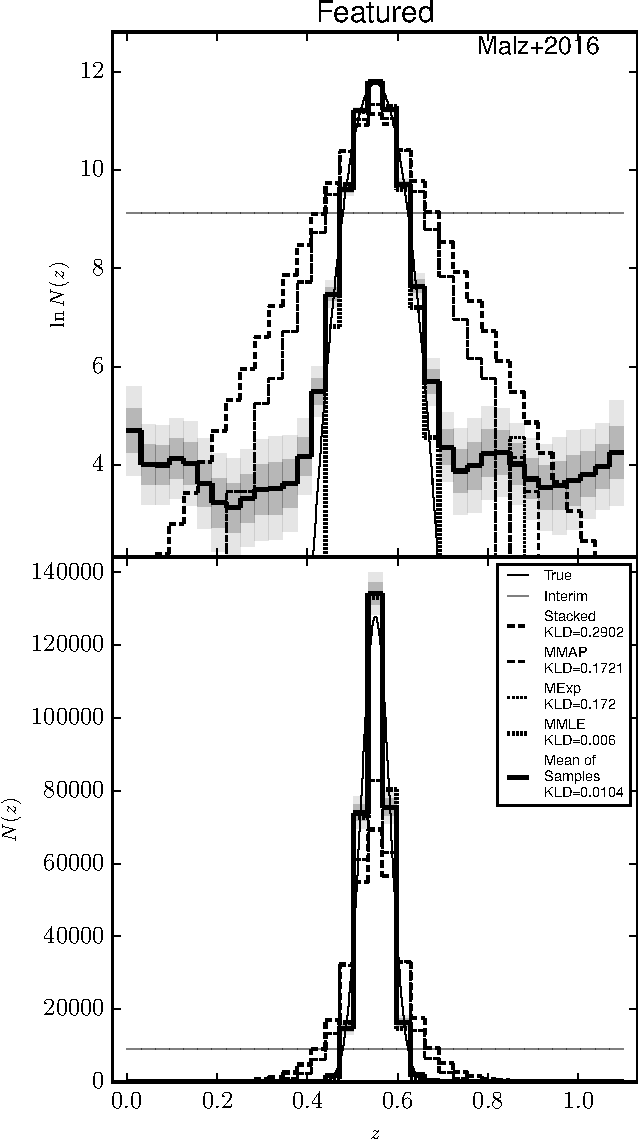
\includegraphics[width=0.5\textwidth]{figures/chippr/delt_comps.pdf}
%	\caption{In this case, the marginalized maximum likelihood estimator (thick, dotted line) recovers the true $N(z)$ (thin, solid line) better than the mean of posterior samples (thick, solid line), though the error bars ($1\sigma$ in dark gray, $2\sigma$ in light gray) do include the true values of the hyperparameters. 
%		The stacked estimator (thick, dashed line) is the worst estimator of the true redshift distribution function, while the marginalized maximum a posteriori estimator (thin, dashed line) and marginalized expected value estimator (thin, dotted line) are not quite as broad.}
%	\figlabel{fig:toy-comp}
%\end{figure}

\subsection{Intrinsic Scatter}
\sectlabel{sec:scatter}

\Fig{fig:pzs-scatter} shows some examples of \pzpdf s generated with only the systematic of intrinsic scatter.
One can see that the histogram of redshift estimates is broader than that of true redshifts, and that the effect is substantially more pronounced by just doubling the intrinsic scatter from the level of the \lsst\ requirements.

\begin{figure}
	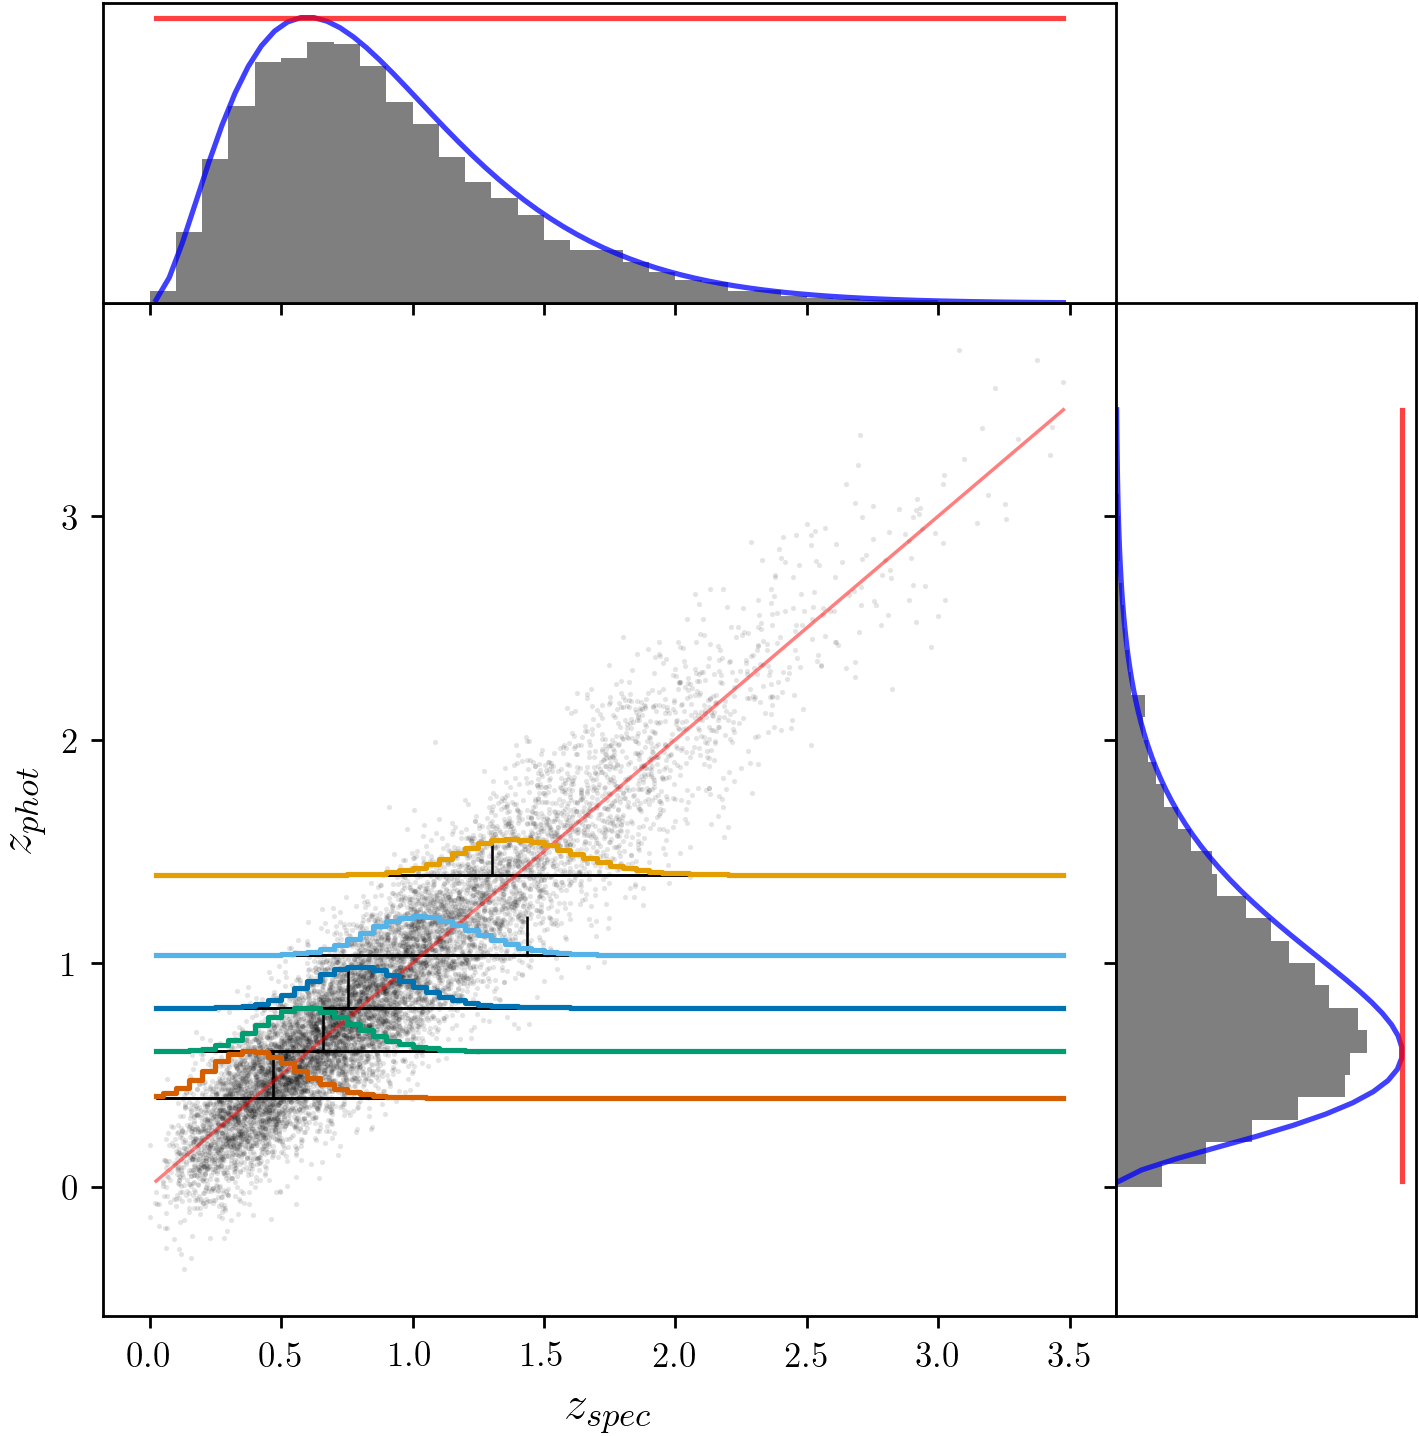
\includegraphics[width=0.5\textwidth]{figures/chippr/samplepzs_scatter1.png}
	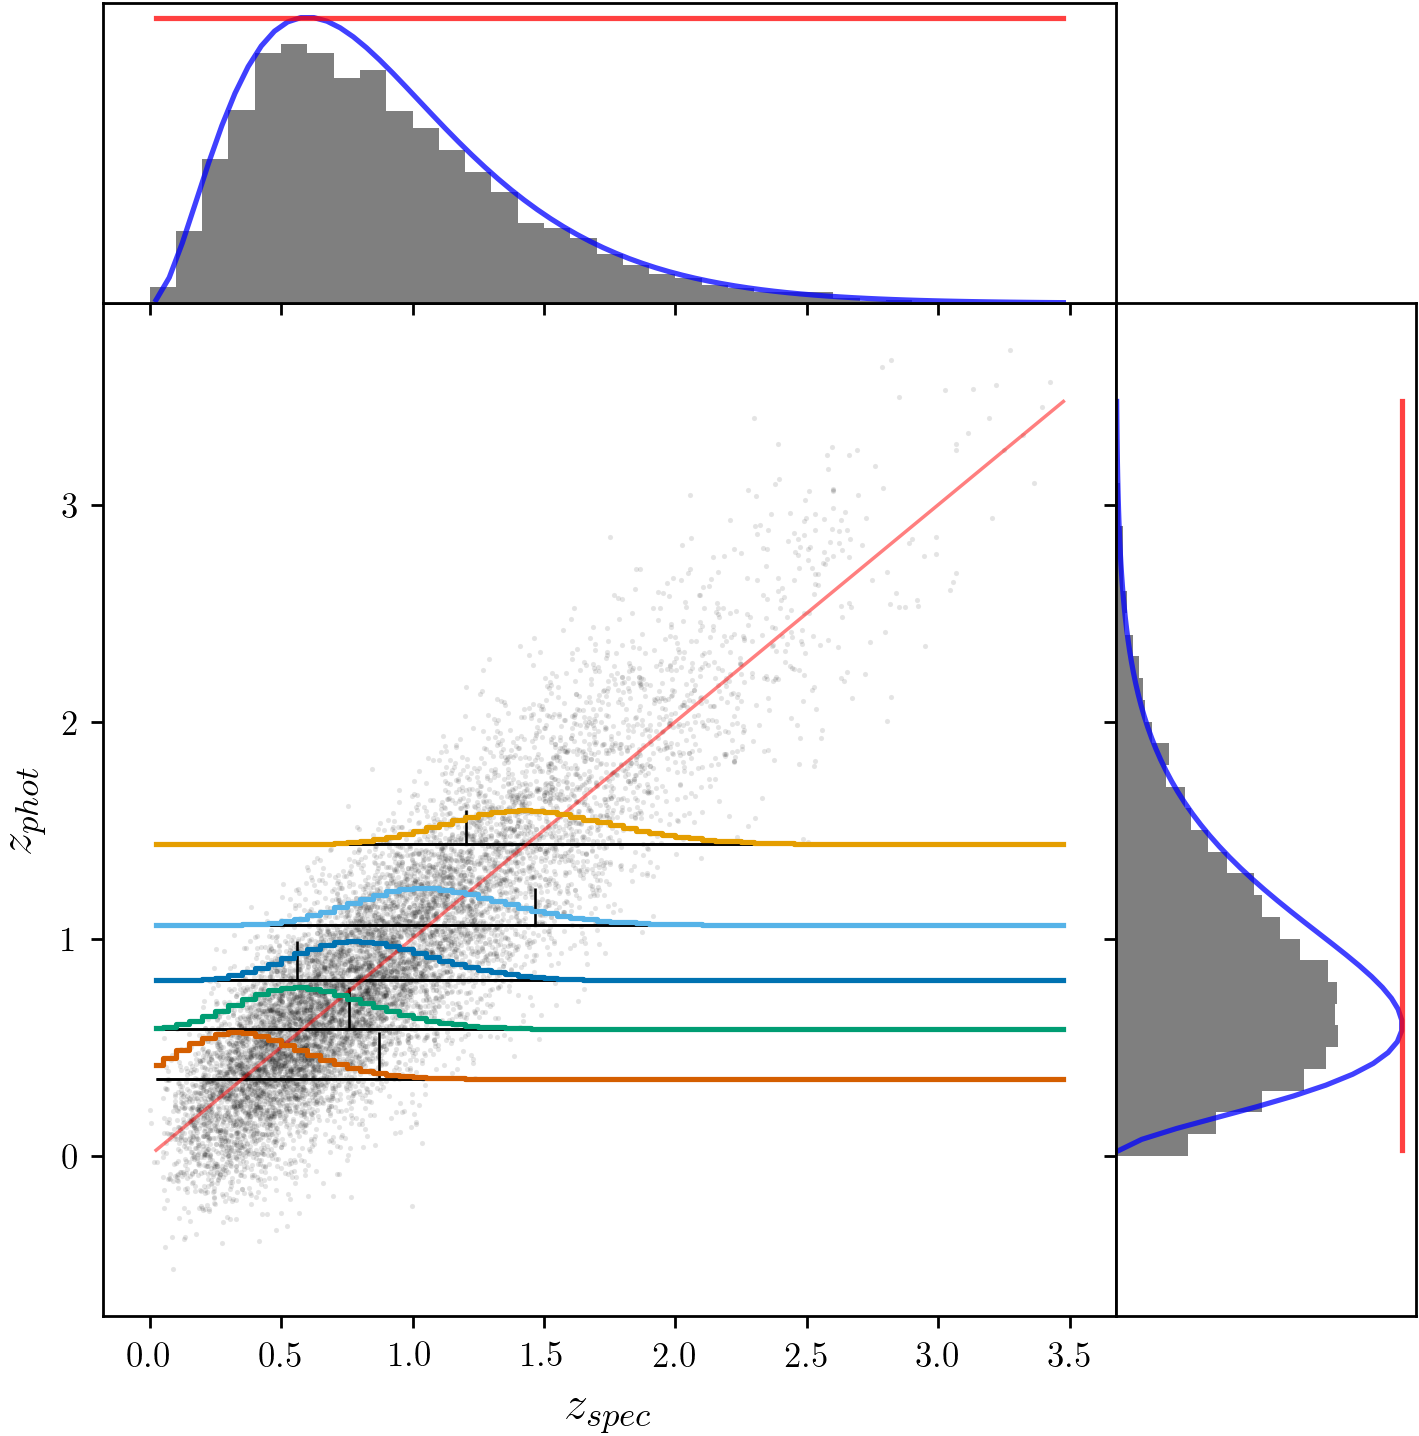
\includegraphics[width=0.5\textwidth]{figures/chippr/samplepzs_scatter2.png}
	\caption{
		Examples of mock \pzpdf s (colored lines) generated with intrinsic scatter at the \lsst\ requirements (left) and twice the \lsst\ requirements (right), including samples from the probability space of true and observed redshift (black points), \pzpdf s (colored lines), the true redshifts of the example \pzpdf s (black vertical lines).
		A histogram (gray) of points in each dimension is shown in the respective inset, with the true redshift distribution (blue curve) and implicit prior (red curve).
	}
	\figlabel{fig:pzs-scatter}
\end{figure}

\Fig{fig:results-scatter} shows the results of \Chippr\ and the alternative approaches.
As expected, the estimates of \nz\ based on the modes of the \pzpdf s and stacking are broader than the marginalized maximum likelihood estimator from \chippr.
Though the marginalized maximum likelihood estimator is unaffected, the \Chippr\ posterior distribution on the redshift distribution is itself broader for the higher intrinsic scatter case than for the \lsst\ requirements.
A broader posterior on \nz\ is an expected consequence of any increase in uncertainty of the \pzpdf s, but the invariance of the marginalized maximum likelihood estimator .

\begin{figure}
	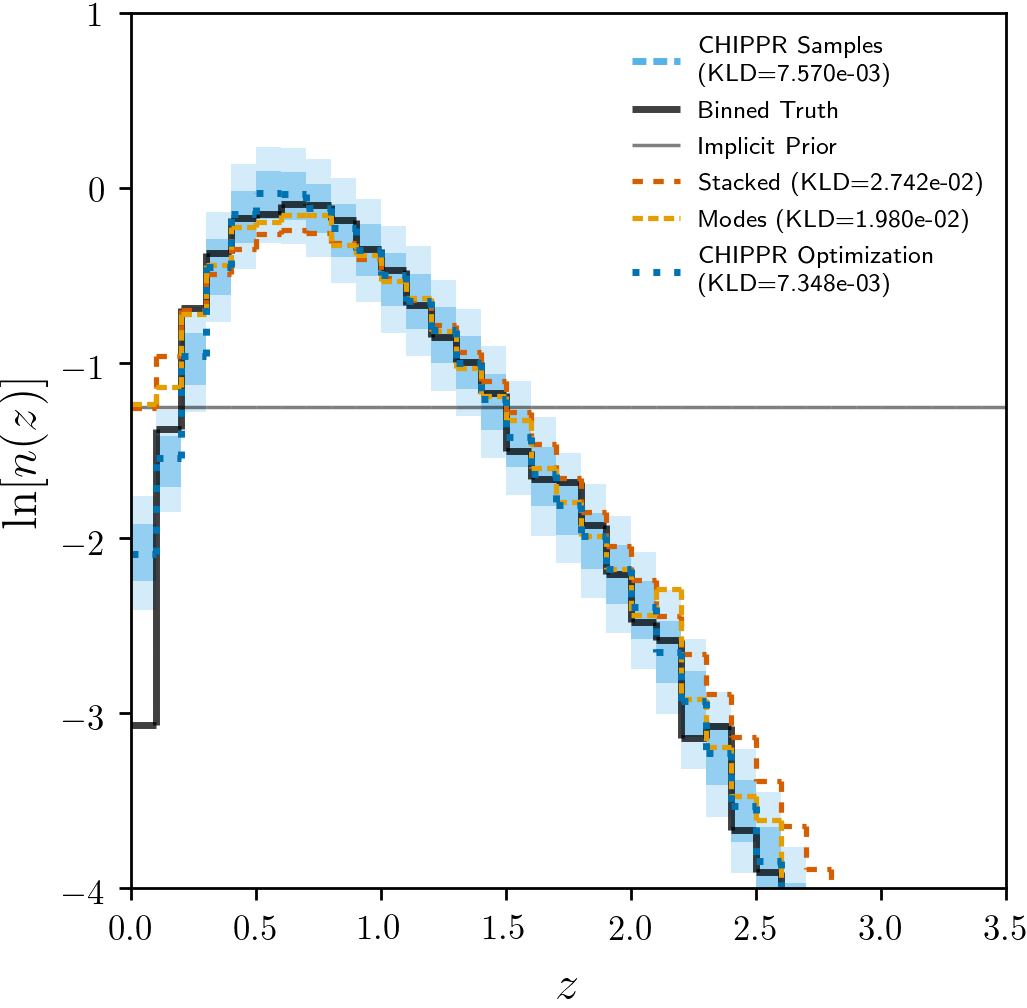
\includegraphics[width=0.5\textwidth]{figures/chippr/results_scatter1.png}
	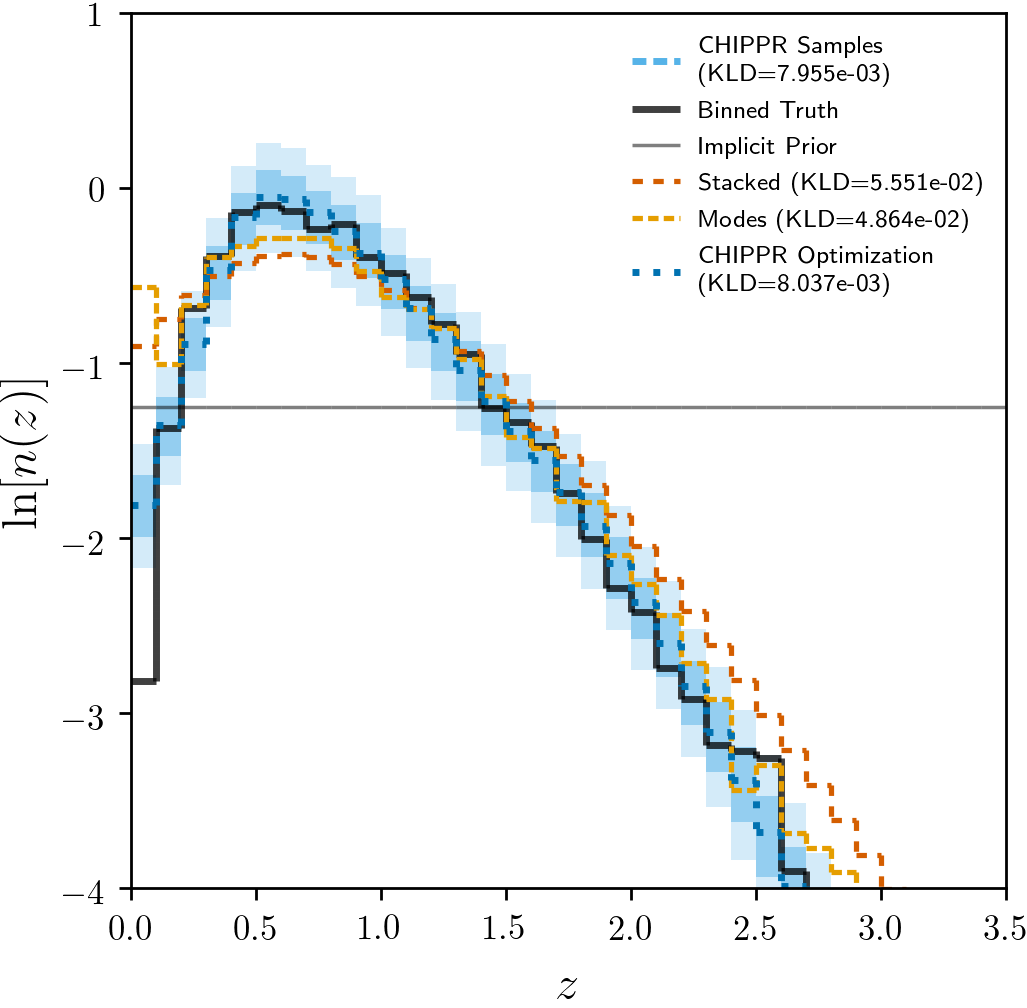
\includegraphics[width=0.5\textwidth]{figures/chippr/results_scatter2.png}
	\caption{
		The results of \Chippr\ (samples in light blue and optimization in dark blue) and the alternative approaches (the stacked estimator in red and the histogram of modes in yellow) on \pzpdf s with intrinsic scatter of the \lsst\ requirements (left) and twice that (right), with the true redshift density (black curve) and implicit prior (gray curve).
		\Chippr\ is robust to intrinsic scatter, but the alternatives suffer from overly broad \nz\ estimates that worsen with increasing intrinsic scatter.
	}
	\figlabel{fig:results-scatter}
\end{figure}

\subsection{Catastrophic Outliers}
\sectlabel{sec:outliers}

As was covered in the Introduction \aim{add an internal reference}, catastrophic outliers tend to be distributed non-uniformly across the space of observed and true redshift.
However, the \lsst\ requirements do not specify details for a distribution of outliers to which they were tuned, and it is still instructive to examine the impact of uniform outliers on the inference of \nz.
More realistic outlier populations will be covered in \Sect{sec:results}.

A uniformly distributed population of outliers was simulated by giving every sample in true redshift a $10\%$ chance of having an observed redshift drawn from a uniform distribution rather than the Gaussian about the true redshift.
Though this results in slightly less than the $10\%$ catastrophic outlier rate, it can be done independently of the definition of the standard deviation so was implemented for demonstrative purposes.
\Fig{fig:uniform-outliers} shows examples of \pzpdf s from a uniformly distributed outlier population at the level of the \lsst\ requirements as well as the results of \Chippr\ and other \nz\ estimation methods.
The alternative estimators are overly broad, whereas \Chippr\ yields an unbiased estimate of \nz.

\begin{figure}
	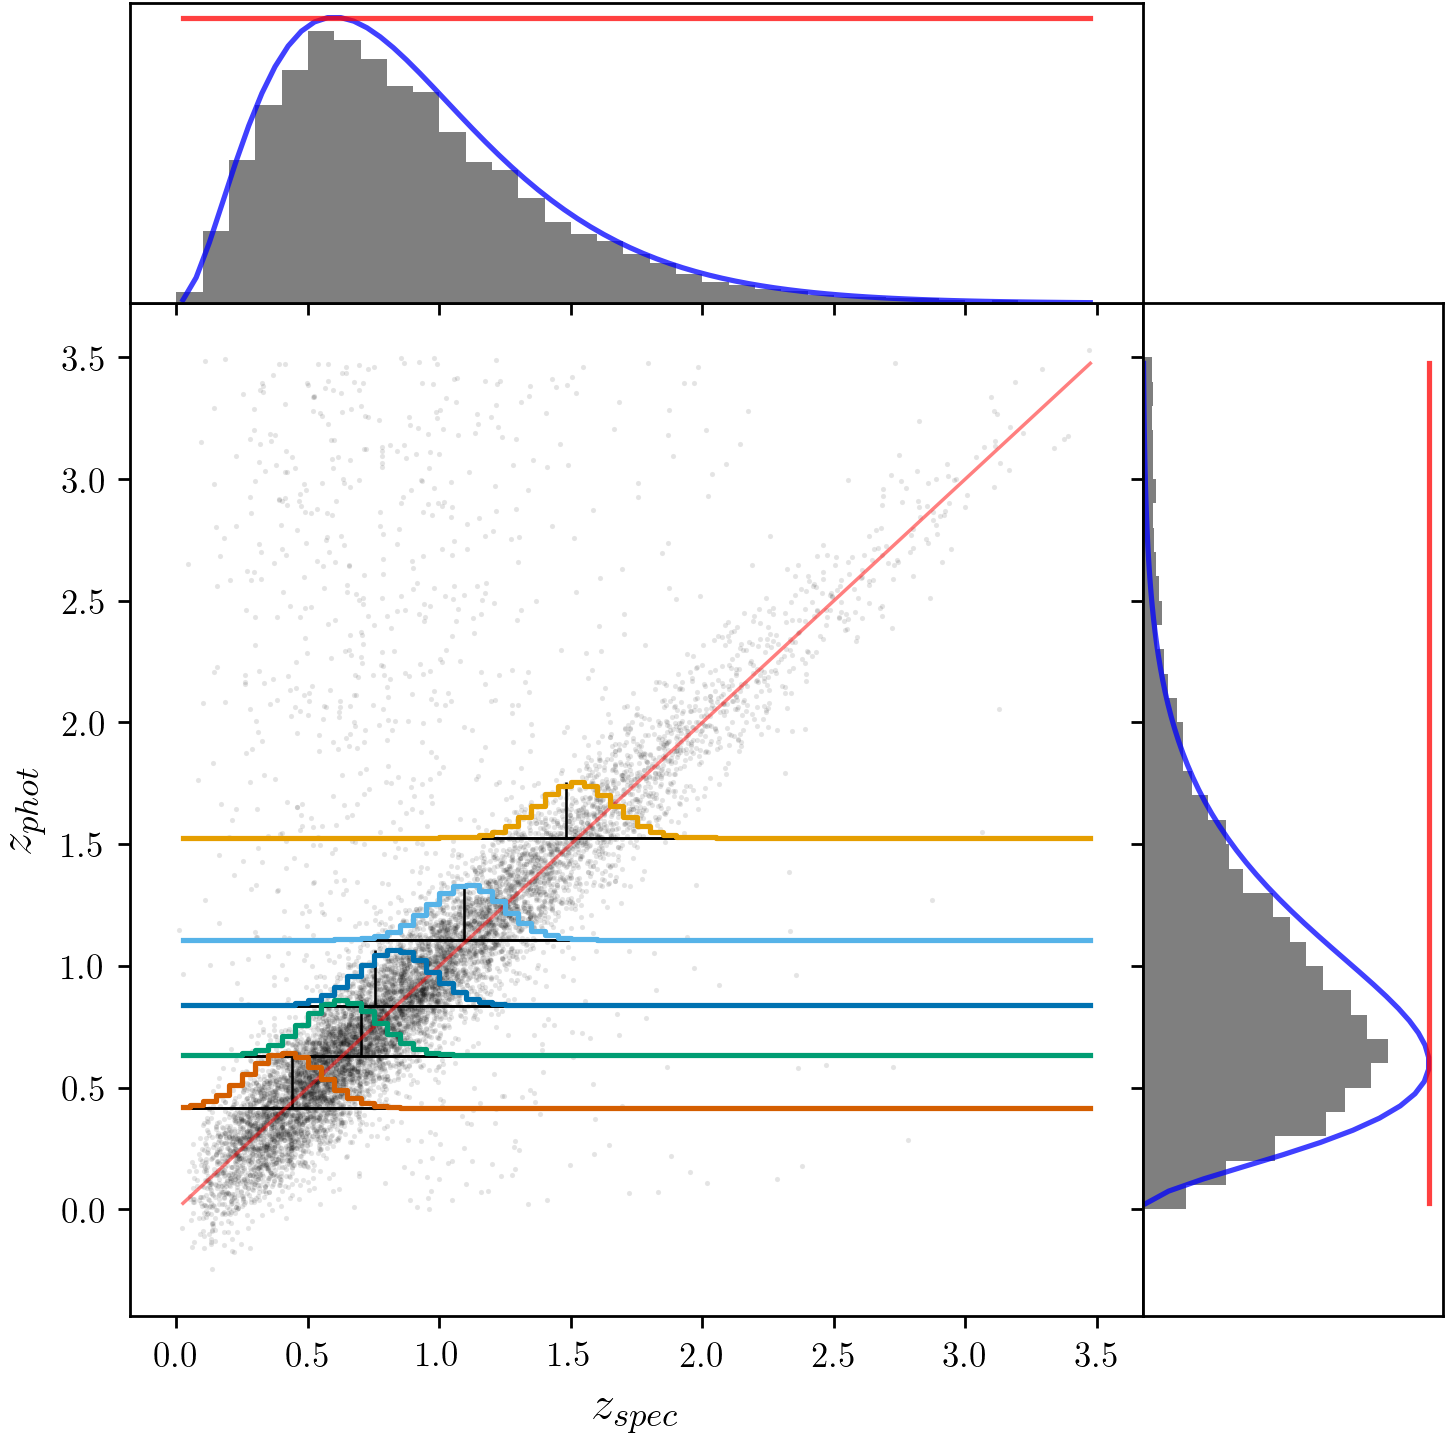
\includegraphics[width=0.5\textwidth]{figures/chippr/single_uout_mega_scatter.png}
	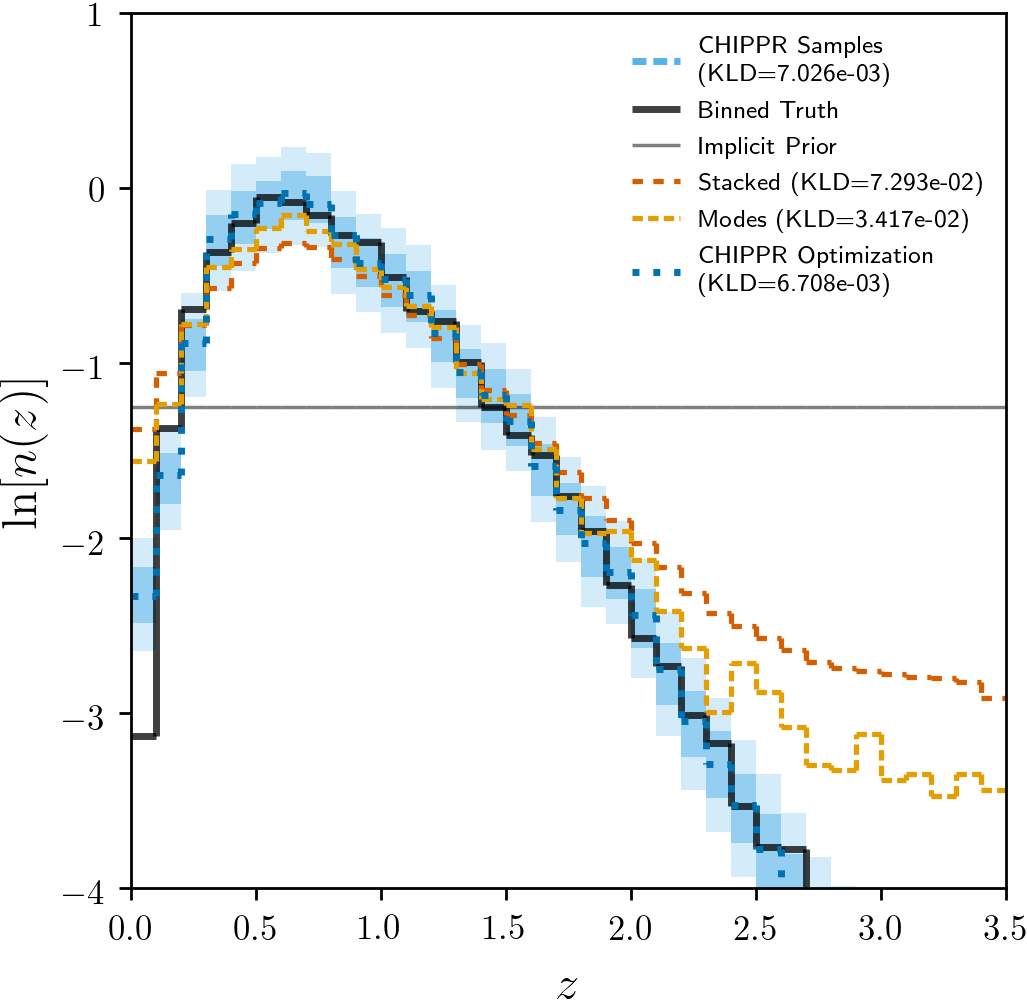
\includegraphics[width=0.5\textwidth]{figures/chippr/single_uout_log_estimators.png}
	\caption{
		Left: Examples of \pzpdf s with a uniform catastrophic outlier population at the level of the \lsst\ requirements, including samples from the probability space of true and observed redshift (black points), \pzpdf s (colored curves), and the true redshifts of the example \pzpdf s (black vertical lines), with marginal histograms (gray) for each dimension with the true redshift distribution (blue curve) and implicit prior (red curve) in the insets.
		Right: The results of \Chippr\ (samples in light blue, optimization in dark blue) and the alternative approaches (the stacked estimator in red, the histogram of modes in yellow) on \pzpdf s with uniformly distributed catastrophic outliers, with the true redshift density (black curve) and implicit prior (gray curve).
		The presence of the catastrophic outlier population broadens the histogram of modes and stacked estimator of the redshift distribution, but the result of \Chippr\ is unbiased.
	}
	\figlabel{fig:uniform-outliers}
\end{figure}

When one thinks of the \pzpdf s of catastrophic outliers, however, what comes to mind is multimodal \pzpdf s, wherein reducing \pzpdf s to point estimates to make a standard scatterplot of the true and observed redshifts leads to substantial probability density off the diagonal.
These coordinated catastrophic outliers may be emulated in the joint probability space of true and estimated redshifts by using a mixture of the unbiased diagonal defined by the intrinsic scatter and an additional Gaussian in one dimension, with constant observed redshift for a template-fitting code and constant true redshift for a machine learning code.
In the case of a catastrophic outlier population like that anticipated of template-fitting codes, $10\%$ of all galaxies have their observed redshift at a particular value unrelated to their true redshift, illustrated in the left panel of \Fig{fig:nonuniform-outliers-data}.
This case is subject to the same caveat as the uniformly distributed outliers when it comes to the \lsst\ requirement.

It is less straightforward to emulate catastrophic outliers like those anticipated of a machine learning code.
The test here gives $10\%$ of galaxies at the redshift affected by outliers an observed redshift that is uniformly distributed relative to the true redshift, illustrated in the right panel of \Fig{fig:nonuniform-outliers-data}.
This means that far fewer than $10\%$ of all galaxies in the sample are catastrophic outliers.
\aim{Probably won't have time to change code to address this inconsistency}
This second variety of outliers is the only kind that can lead to multimodal \pzpdf s under the forward model.
\aim{Interpret this in terms of whether BPZ, etc. are yielding likelihoods and how it relates to the standard true vs. estimated redshift plot presented in the introduction.}

\begin{figure}
	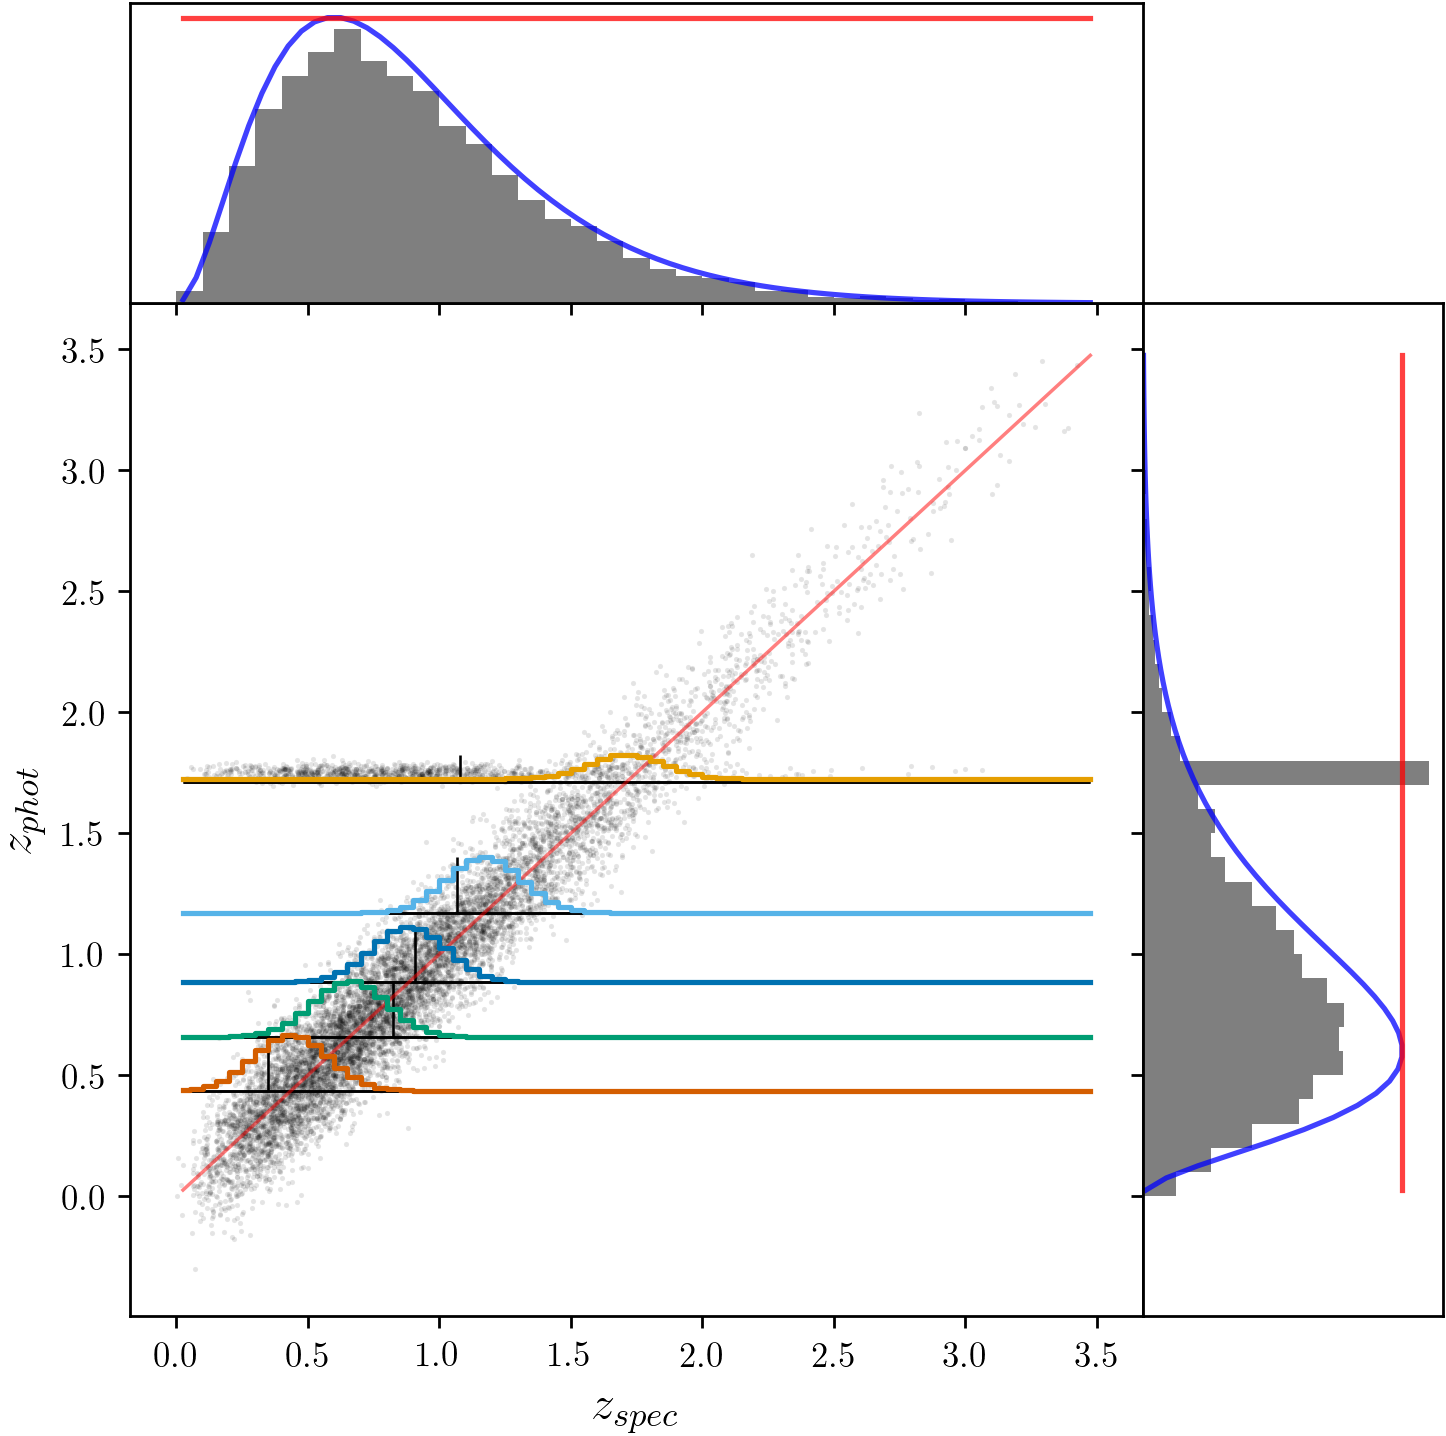
\includegraphics[width=0.5\textwidth]{figures/chippr/thesis_eout_mega_scatter.png}
	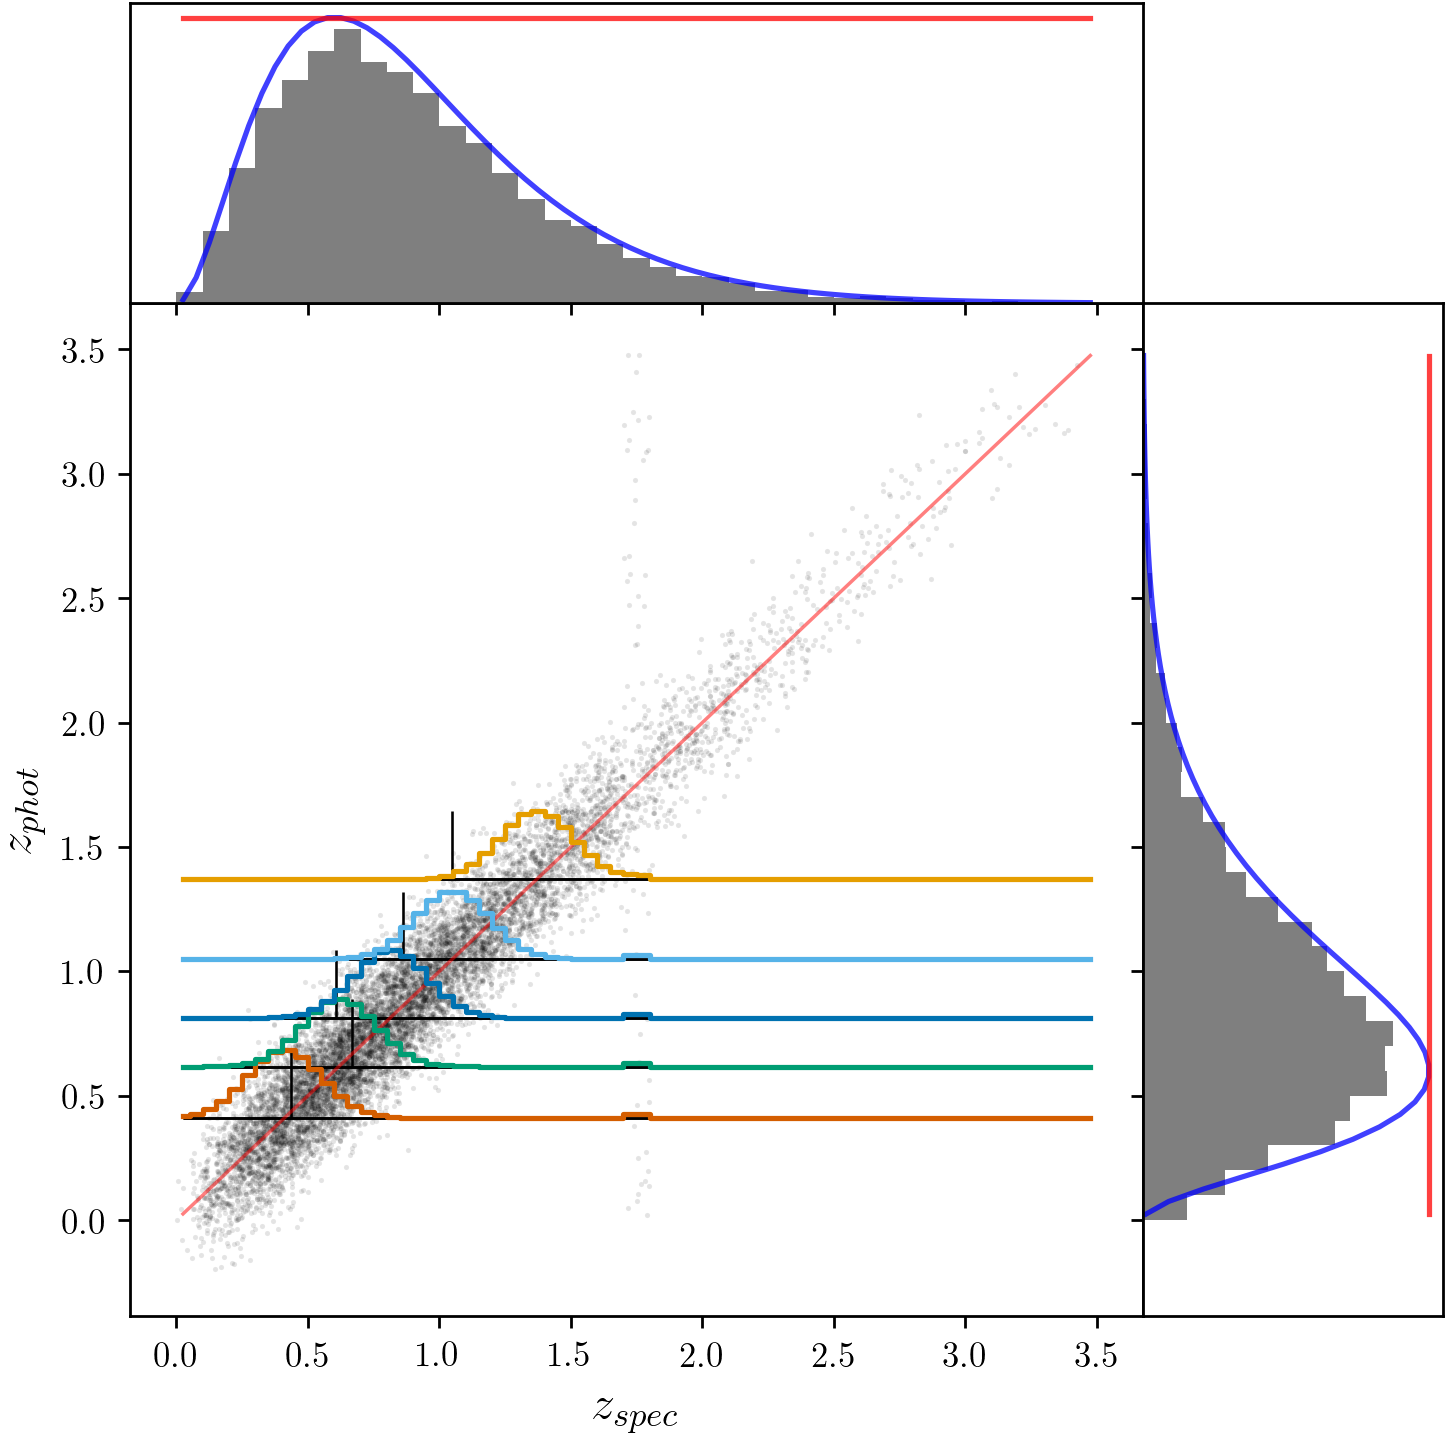
\includegraphics[width=0.5\textwidth]{figures/chippr/thesis_rout_mega_scatter.png}
	\caption{
		Examples of \pzpdf s with a catastrophic outlier population like that seen in template-fitting \pzpdf\ codes (left) and machine learning \pzpdf\ codes (right), including samples from the probability space of true and observed redshift (black points), \pzpdf s (colored curves), and the true redshifts of the example \pzpdf s (black vertical lines), with marginal histograms (gray) for each dimension with the true redshift distribution (blue curve) and implicit prior (red curve) in the insets.
	}
	\figlabel{fig:nonuniform-outliers-data}
\end{figure}

The results of \Chippr\ and the alternative estimators of \nz\ are presented in \Fig{fig:nonuniform-outliers-results}.
The most striking feature is that the histogram of modes is highly sensitive to the outlier populations, producing a severe overestimate in the case of an outlier population like those seen in template-fitting codes and a severe underestimate in the case of an outlier population like those seen in machine learning codes.
The effect on the stacked estimator of \nz\ is more subtle though still concerning.
In the case of outliers like those resulting from template-fitting, the estimator is overly broad, and in the case of outliers like those resulting from machine learning, the estimator features an overestimate at the redshift affected by the outlier population.
The \Chippr\ \mmle, however, appears unbiased and withstands these effects.

\begin{figure}
	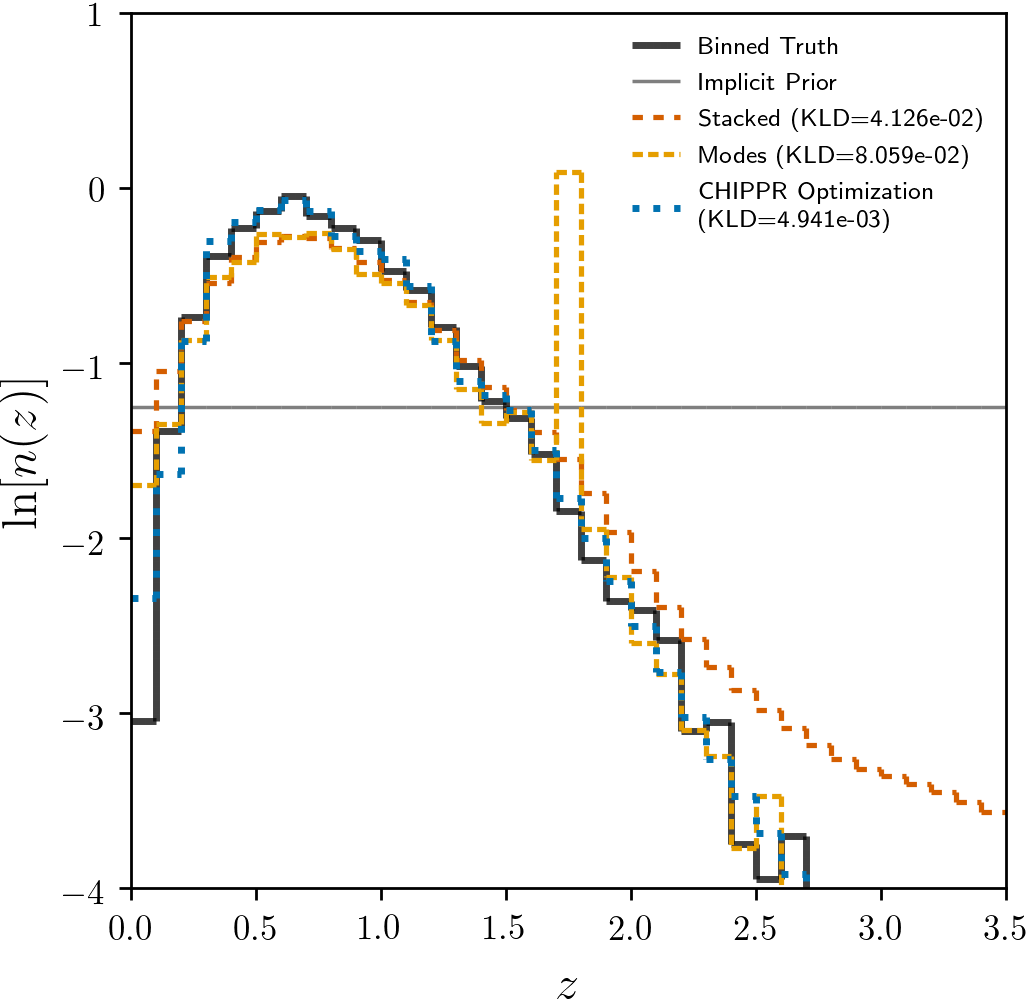
\includegraphics[width=0.5\textwidth]{figures/chippr/thesis_eout_log_estimators.png}
	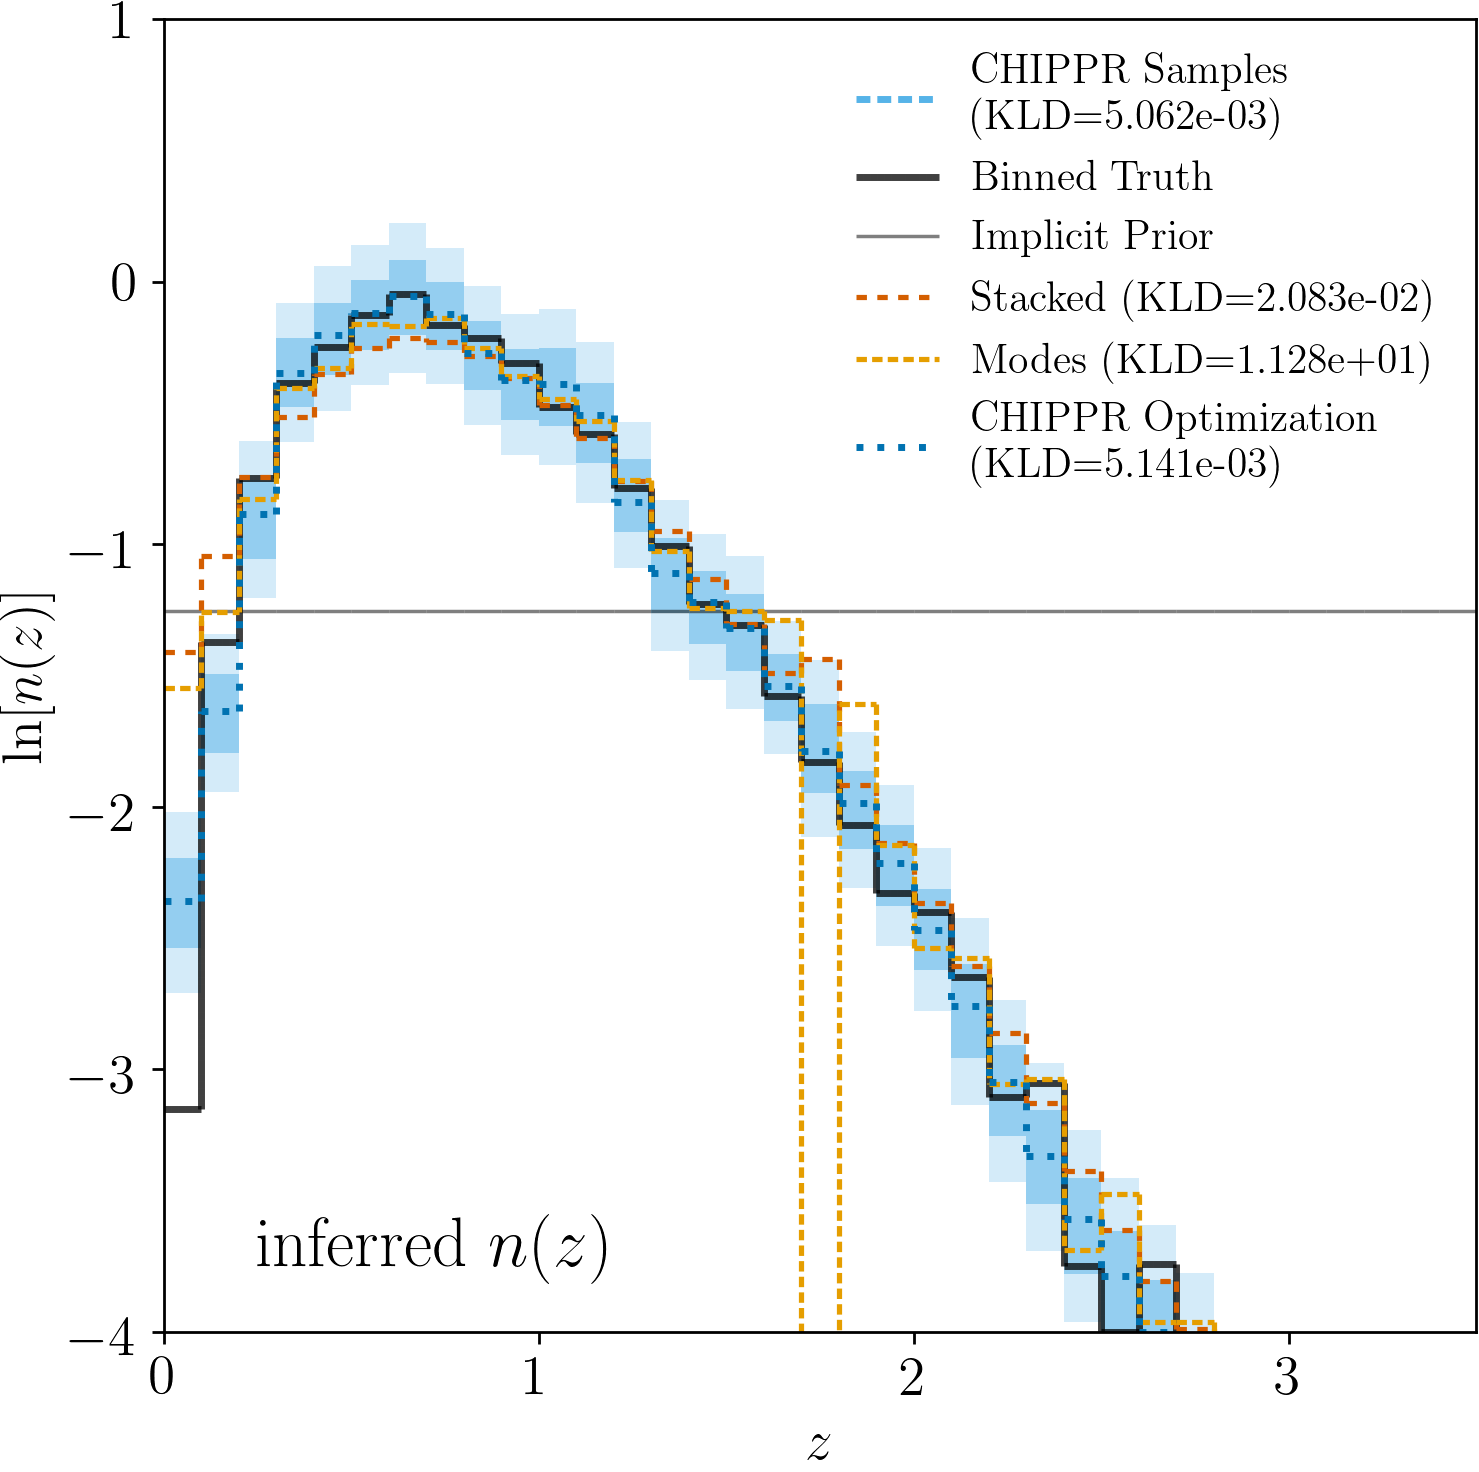
\includegraphics[width=0.5\textwidth]{figures/chippr/thesis_rout_log_estimators.png}
	\caption{
		The results of \Chippr\ (samples in light blue and optimization in dark blue) and the alternative approaches (the stacked estimator in red, the histogram of modes in yellow) on \pzpdf s with catastrophic outliers like those seen in template-fitting \pzpdf\ codes (left) and machine learning \pzpdf\ codes (right) to the \lsst\ requirements, with the true redshift density (black curve) and implicit prior (gray curve).
		Though the histogram of modes is most sensitive to a catastrophic outlier population, the stacked estimator also overestimates \nz\ under (machine learning-like outliers) and beyond (template fitting-like outliers).
	}
	\figlabel{fig:nonuniform-outliers-results}
\end{figure}

\subsection{Bias}
\sectlabel{sec:bias}

The notion of redshift bias is a form of model misspecification.

\aim{Include the tests here?
They're trivial but might be worth explaining.}

\subsection{Nontrivial implicit prior}
\sectlabel{sec:interim}

\Chippr\ can handle any implicit prior with support over the redshift range where \nz is defined, but some archetypes of implicit prior are more likely to be encountered in the wilds of \pzpdf\ codes.
Ideally, an uninformative implicit prior would be used, although it may be complicated to compute from the covariances of the raw data.  
Template-fitting codes have an explicit prior input formed by redshifting a small number of templates, leading to a highly nonuniform but physically-motivated interim prior.
%Another potential method for selecting an interim prior with support over the entire redshift range expected of the photometric survey is to sum two or more $N(z)$ distributions obtained from reliable photometric surveys in the past.  
%This is just as problematic as using a biased spectroscopically derived $N(z)$ as the interim prior because the sum of redshift distributions for two or more surveys does not reflect our beliefs about the true distribution for a single survey even though it provides support over the same redshift range.  
%To simulate this case, we choose an interim prior with more weight at high and low redshifts than for mid-range redshifts.  
Machine learning approaches tend to be trained on previously observed data sets that are biased towards low redshift, which biases the implicit prior towards low redshift.
Some efforts have been made to modify an observationally informed implicit prior so that it is more representative of the photometric data for which redshifts are desired \citep{Sheldon2012}, but, unless it is equal to the true \nz, it will propagate to the results of traditional \nz\ estimation methods.  
%Because low-redshift galaxies are more likely to be bright enough to be observed by such a survey, $N(z)$ determined from that sample may be heavily biased to low redshift galaxies.  
%By contrast, the galaxies that were unobserved in such a survey are more likely be dimmer, making them more likely to be at higher redshifts.  
%Since the interim prior is not compatible with our beliefs about the true redshift distribution, the resulting interim redshift posteriors will be inappropriate.  

\Fig{fig:pzs-priors} shows examples of \pzpdf s with a low-redshift favoring implicit prior emulating that of a machine learning approach to \pz\ estimation and a more complex interim prior emulating that of a template-fitting \pz\ method.
One can see that the \pzpdf s take different shapes from one another even though the marginal histograms are identical.

\begin{figure}
	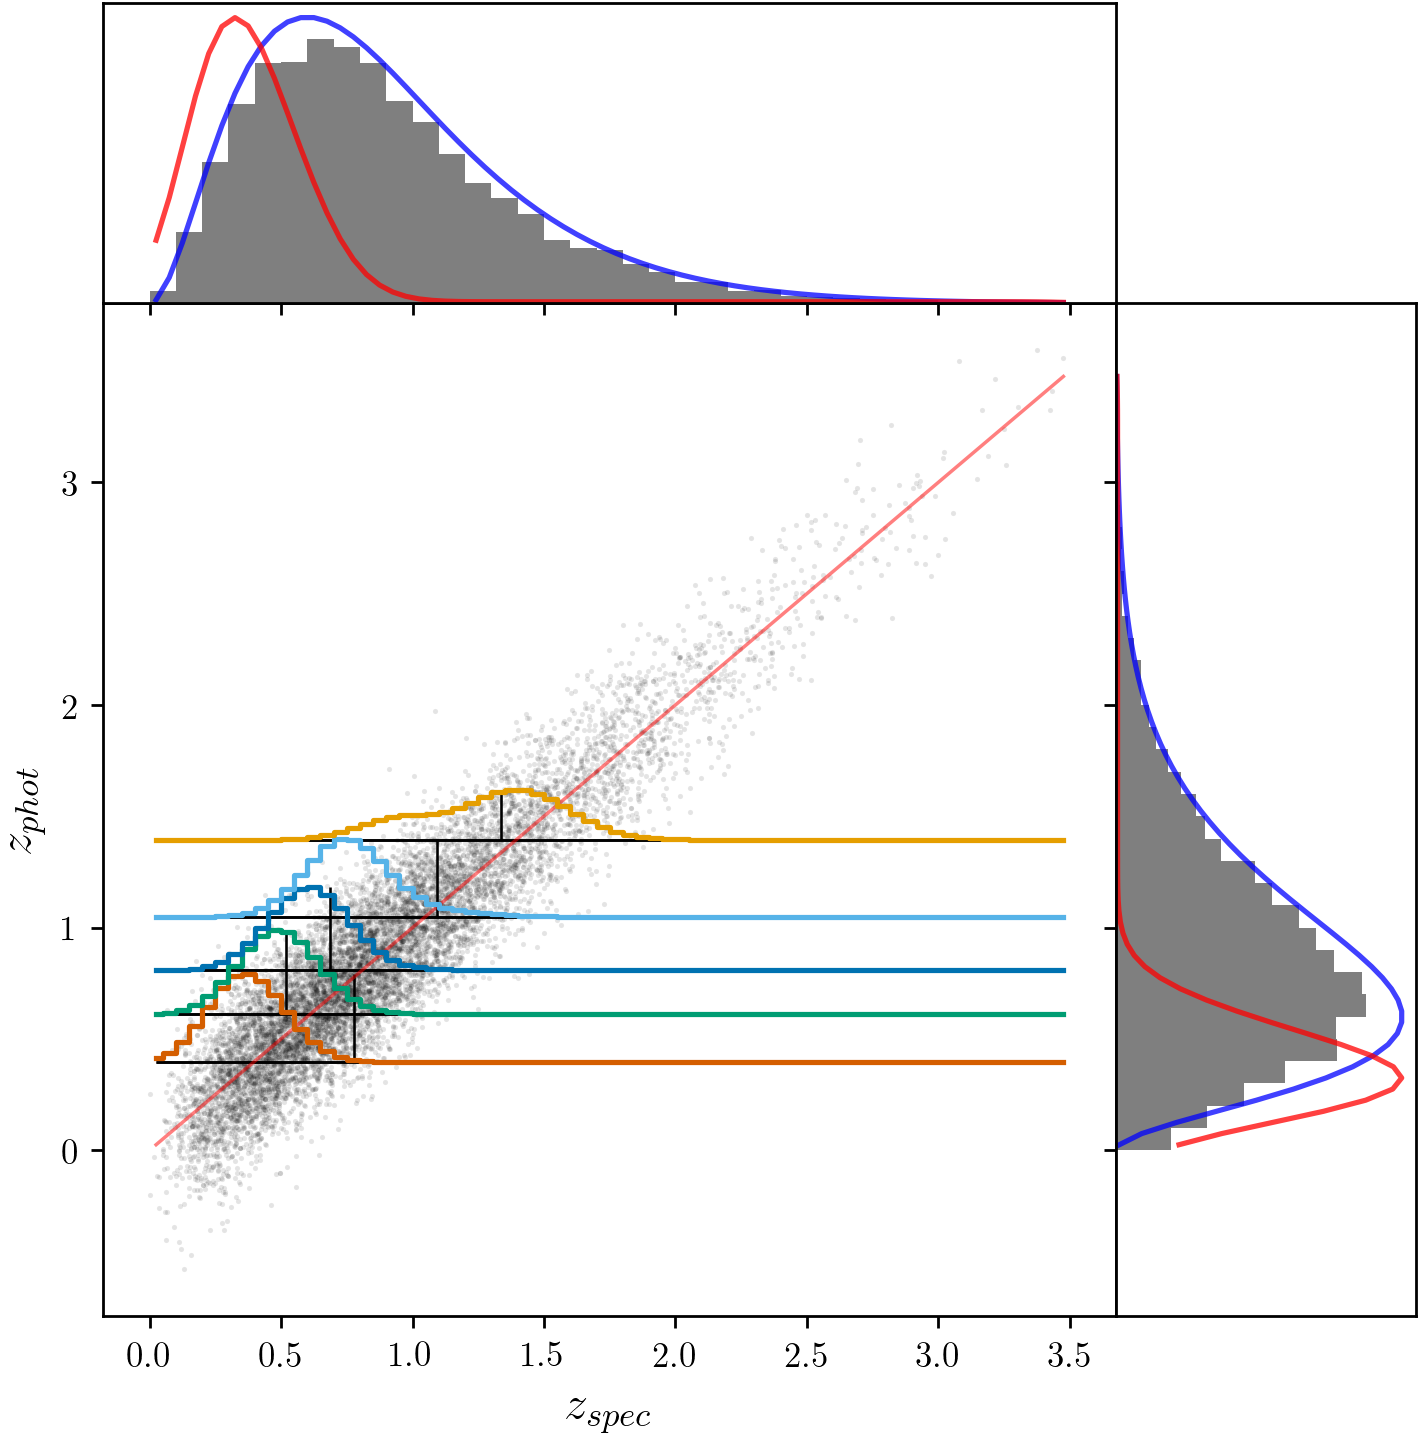
\includegraphics[width=0.5\textwidth]{figures/chippr/samplepzs_trpr.png}
	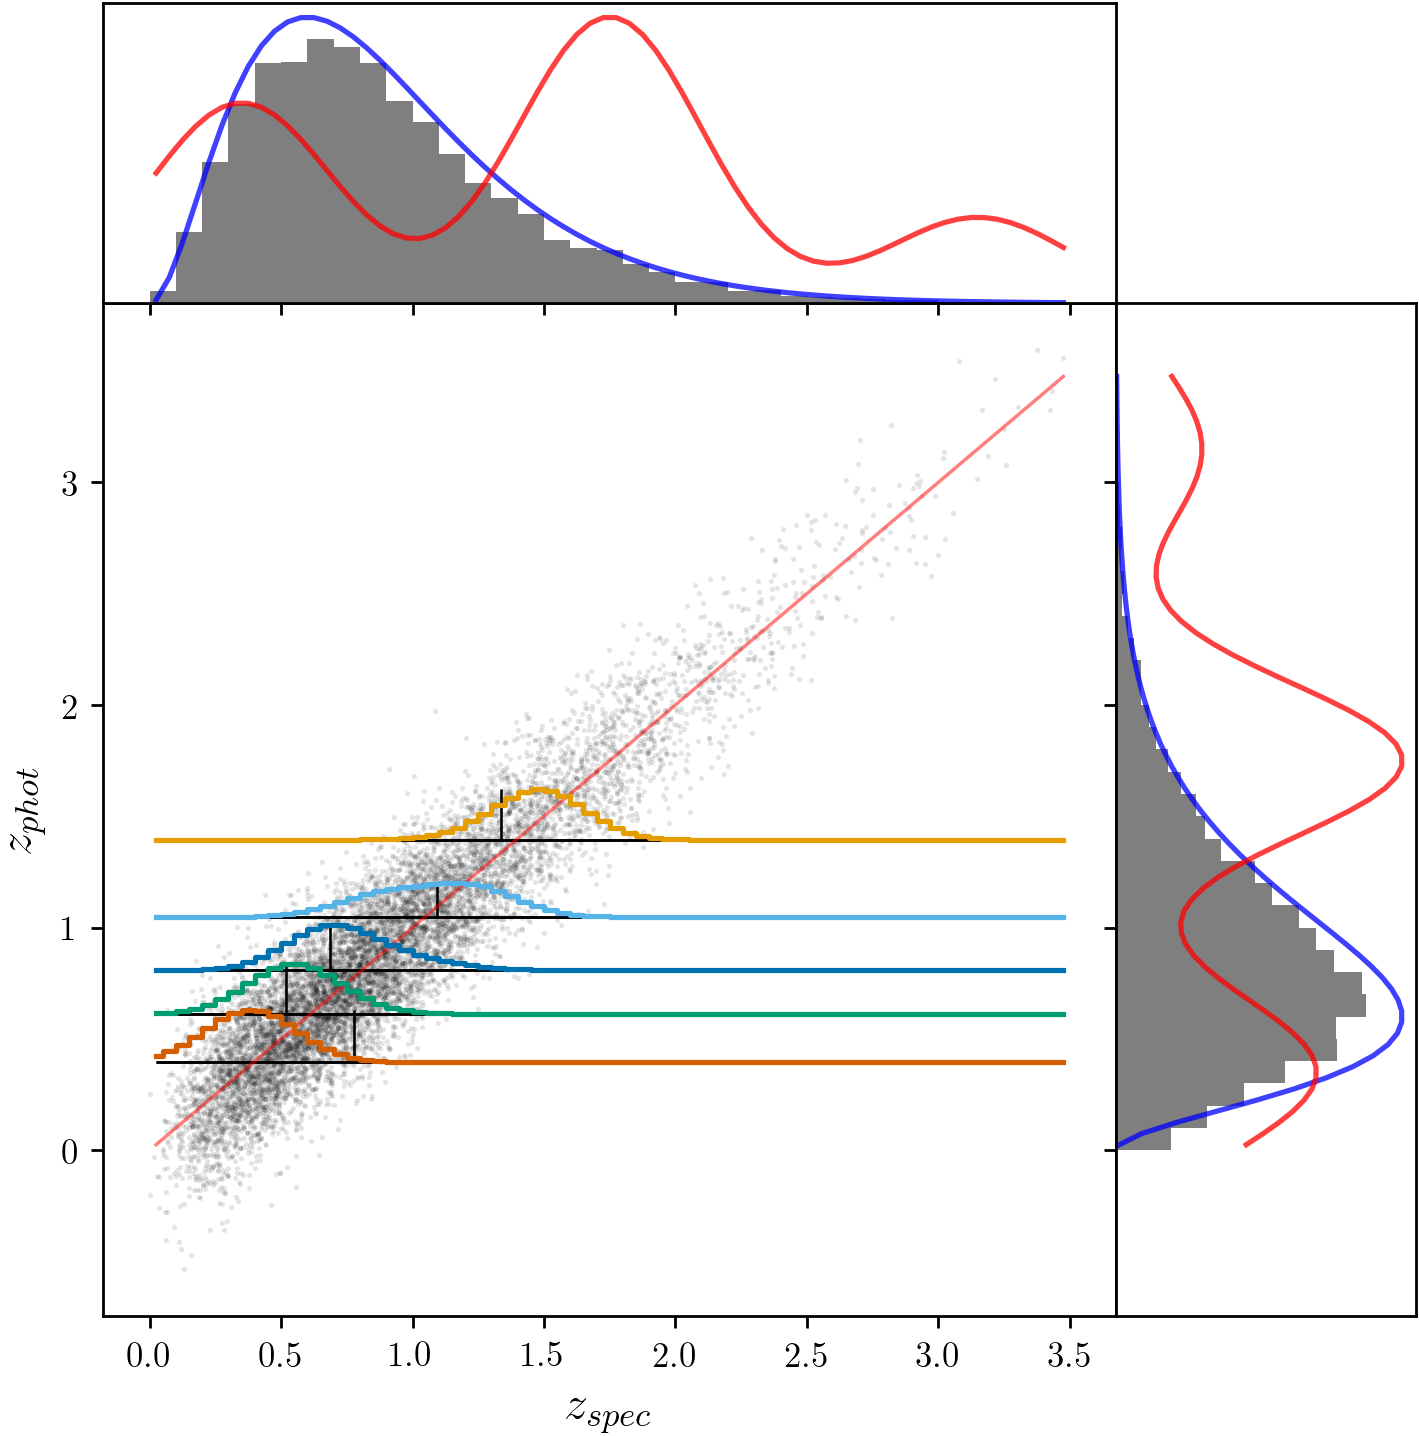
\includegraphics[width=0.5\textwidth]{figures/chippr/samplepzs_tmpr.png}
	\caption{
		Examples of mock \pzpdf s (colored lines) generated with a machine learning-like implicit prior (left) and a template-fitting-like implicit prior (right), including samples from the probability space of true and observed redshift (black points), \pzpdf s (colored lines), the true redshifts of the example \pzpdf s (black vertical lines).
		A histogram (gray) of points in each dimension is shown in the respective inset, with the true redshift distribution (blue curve) and implicit prior (red curve).
	}
	\figlabel{fig:pzs-priors}
\end{figure}

\Fig{fig:results-priors} shows the performance of \Chippr\ and the traditional methods on \pzpdf s generated with nontrivial implicit priors.
In both cases, the \Chippr\ \mmle\ effectively recovers the true redshift distribution.
The alternatives, however, are biased by the implicit prior except where it is flat, in the case of high redshifts for the machine learning-like implicit prior.
\aim{Show that this gets worse for higher intrinsic scatter as well?}

\begin{figure}
	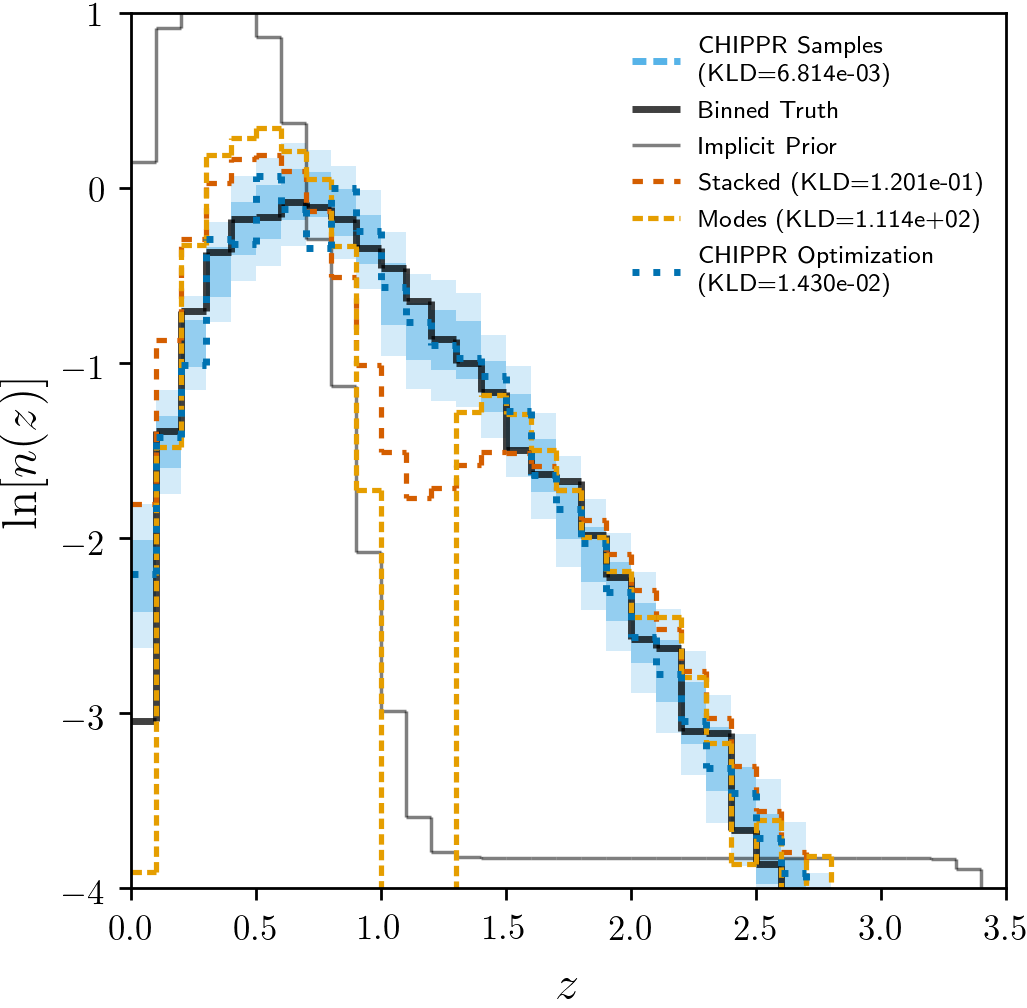
\includegraphics[width=0.5\textwidth]{figures/chippr/results_trpr.png}
	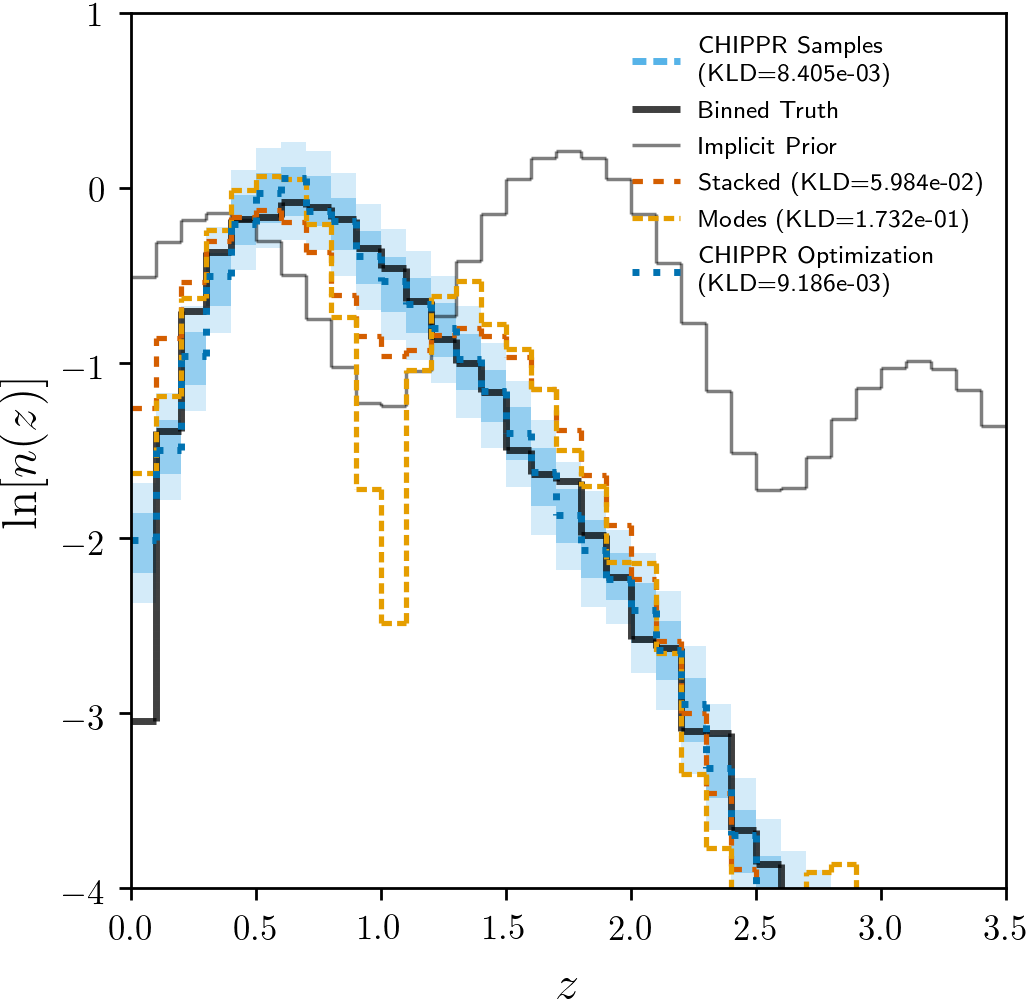
\includegraphics[width=0.5\textwidth]{figures/chippr/results_tmpr.png}
	\caption{
		The results of \Chippr\ (samples in light blue and optimization in dark blue) and the alternative approaches (the stacked estimator in red and the histogram of modes in yellow) on \pzpdf s with an implicit prior like that of machine learning \pzpdf\ approaches (left) and an implicit prior like that of template-fitting \pzpdf\ codes (right), with the true redshift density (black curve) and implicit prior (gray curve).
		\Chippr\ is robust to a nontrivial implicit prior, but the alternatives are biased toward the implicit prior.
	}
	\figlabel{fig:results-priors}
\end{figure}

\section{Discussion}
\sectlabel{sec:results}

\aim{I still need to write the intro to the big LSST-like forecast and incorrect implicit prior sections.}

\aim{Q: How does the result of \chippr\ compare to established estimators in terms of the accuracy of $n(z)$?\\
	A: \chippr\ yields the best possible $n(z)$, conditional on the accuracy of the photo-$z$ PDFs used.}

\aim{Include quantitative results on KLD of \Nz\ and cosmological parameter space.}

\subsection{LSST Requirements}
\sectlabel{sec:lsstdemo}

To test the impact of these uncertainties, we simulated mock data with all three effects and did a Fisher matrix forecast using \cosmolike.
\aim{Cite CosmoLike.}

\begin{figure*}
	\begin{center}
		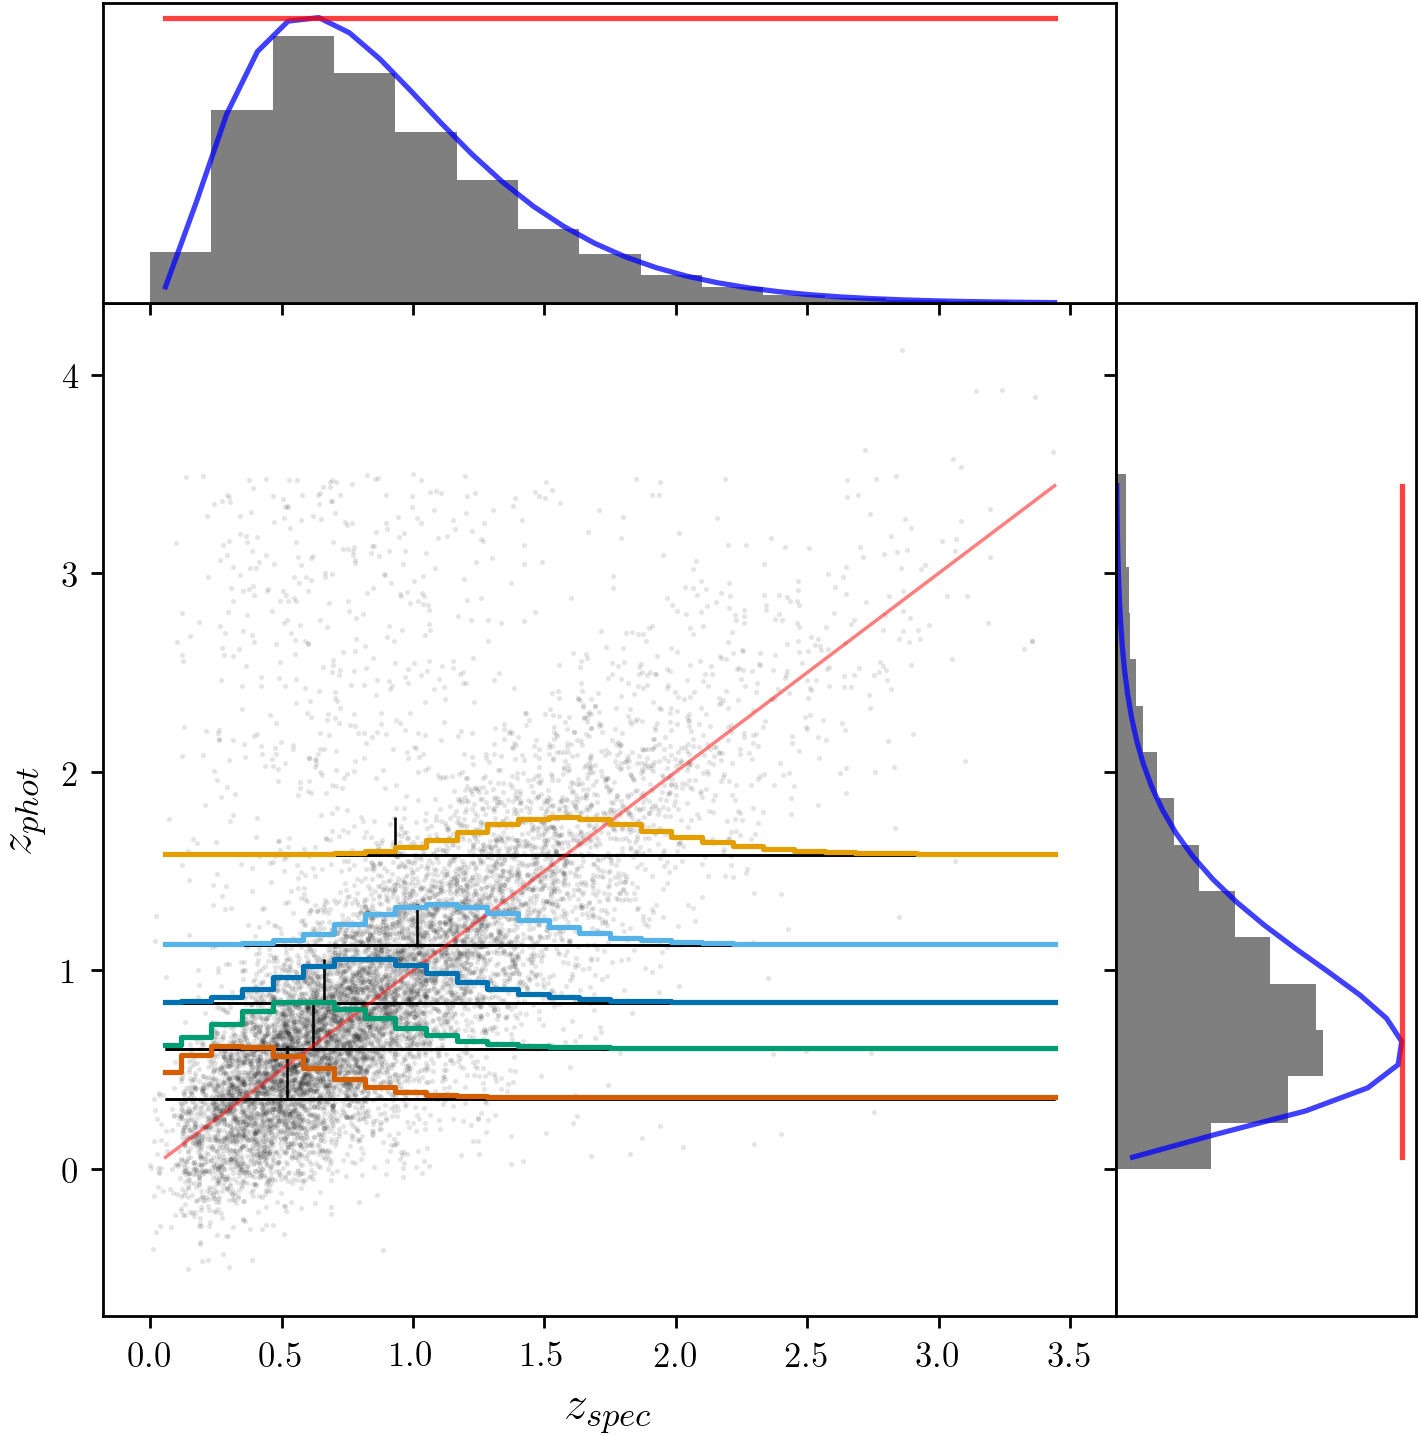
\includegraphics[width=0.45\textwidth]{figures/chippr/lsst_scatter.png}
		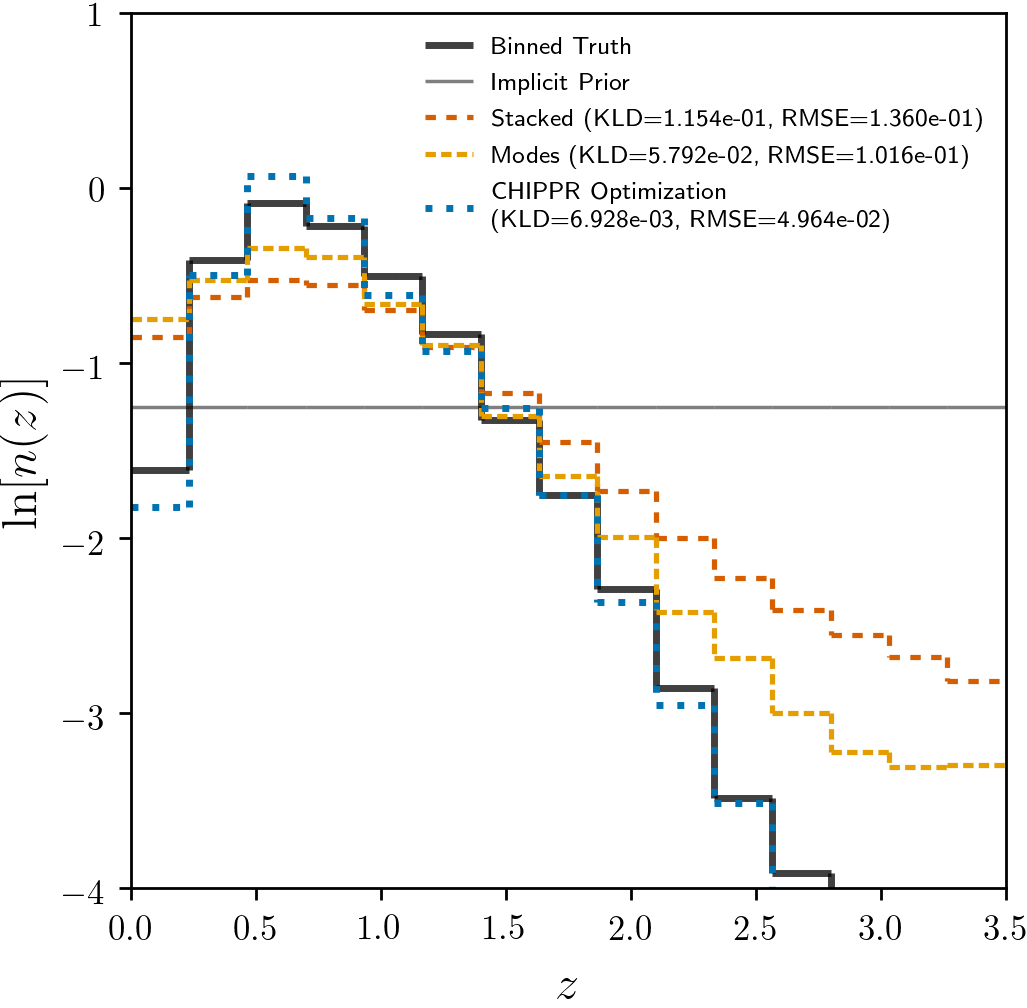
\includegraphics[width=0.45\textwidth]{figures/chippr/lsst_log_estimators.png}
		\caption{T
		\aim{Rerun this with 35 bins and sampling to match other figures.}}
		\figlabel{fig:lsstdemo}
	\end{center}
\end{figure*}

It is of interest to explore the impact of incorrectly estimated \nz\ on the inference of the cosmological parameters to answer the question of how wrong we will be in our understanding of the universe if we don't perform a valid inference.
To find an answer, I considered a set of tomographically binned \nz\ and cosmological parameter covariance matrices used for \desc\ forecasting, for which the true \nz\ in each pre-defined bin is already provided in the form of an evaluation of a function on a fine grid of $350$ redshifts $0.0101 < z < 3.5001$.
First, I binned them down to a piecewise constant parameterization with a manageable $35$ parameters for \chippr's sampling capabilities.
Next, I drew $10^{4}$ true redshifts from the binned true \nz\ for each tomographic bin.
The original, binned, and drawn \nz\ are shown in \Fig{fig:tomobins}

\begin{figure*}
	\begin{center}
		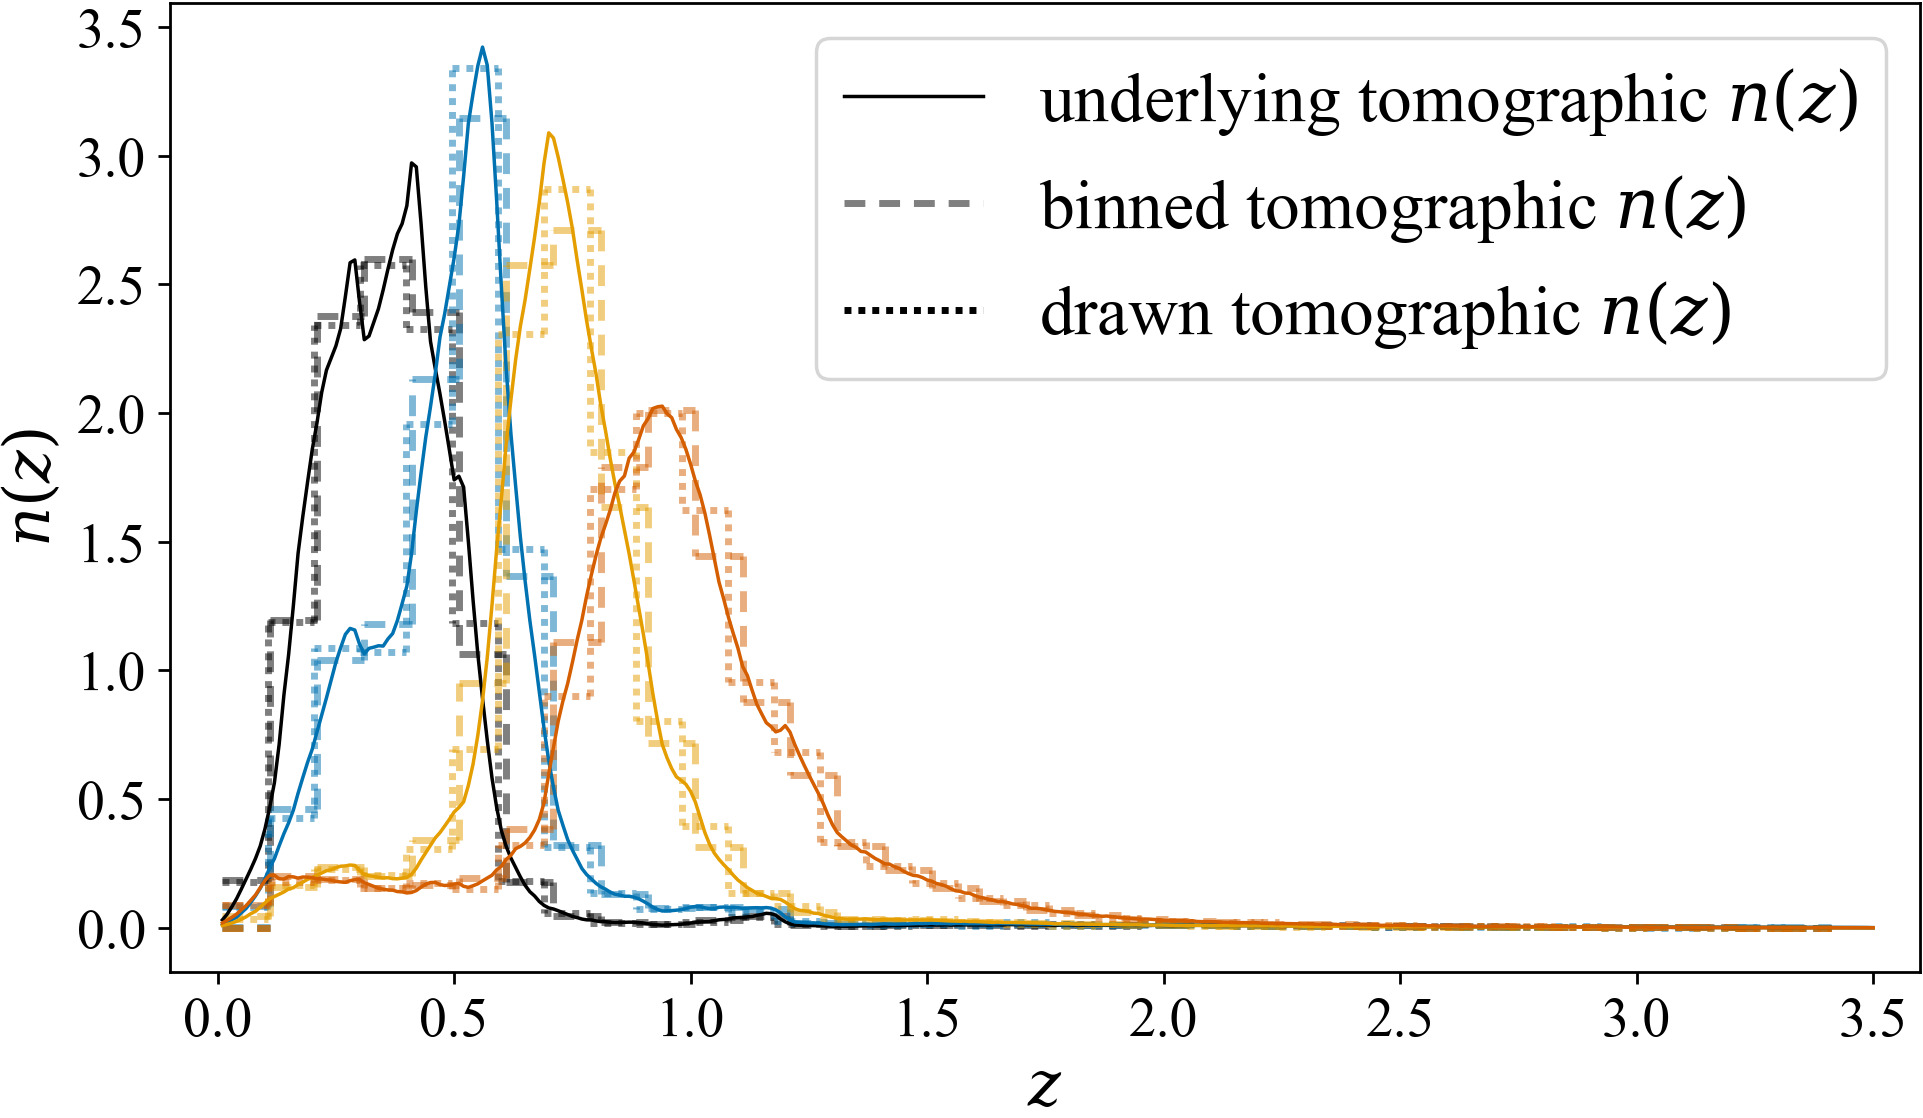
\includegraphics[width=0.74\textwidth]{figures/chippr/cosmolike_inputs.png}
		\caption{The \lsst-like tomographic binning and true redshift distribution, where the truth (solid) is a PDF evaluated on a fine grid of $350$ redshifts $0.0101 < z < 3.5001$, and the binned (dashed) and drawn (dotted) \nz\ are piecewise constant functions evaluated in $35$ evenly spaced bins.
		}
		\figlabel{fig:tomobins}
	\end{center}
\end{figure*}

Using the \lsst\ \pz\ requirements given in \Sect{sec:lsstdemo}, I emulated \pzpdf s corresponding to the $10^{4}$ true redshifts drawn from the true \nz\ in each bin using the procedure of \Fig{fig:flowchart}.
I then ran \chippr\ as well as the two other \nz\ estimation methods on the \pzpdf\ catalog for each tomographic bin.
The estimates are given in \Fig{fig:per-bin-ests}.
One can see that the excessive breadth of the stacked estimator and the histogram of the modes of the \pzpdf s.

\begin{figure*}
	\begin{center}
		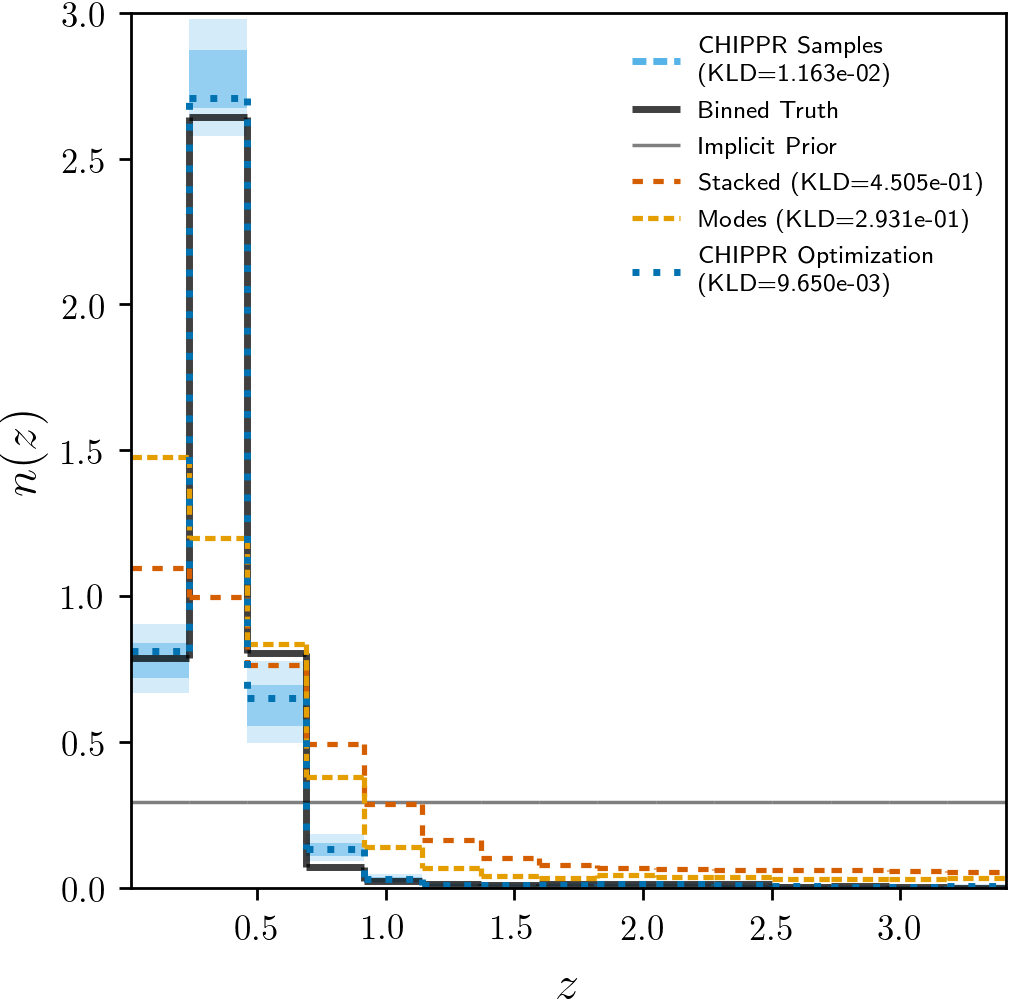
\includegraphics[width=0.24\textwidth]{figures/chippr/0single_lsst_lin_estimators.png}
		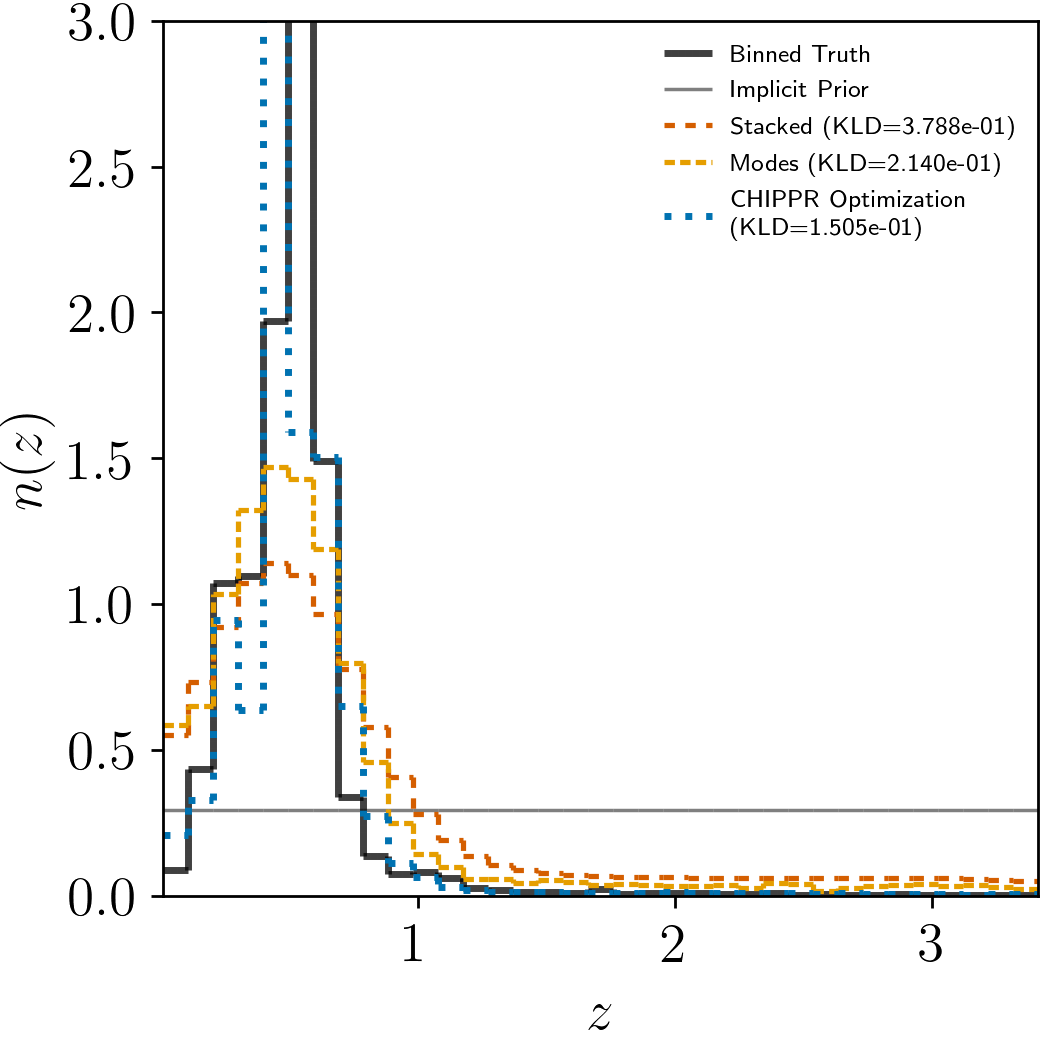
\includegraphics[width=0.24\textwidth]{figures/chippr/1single_lsst_lin_estimators.png}		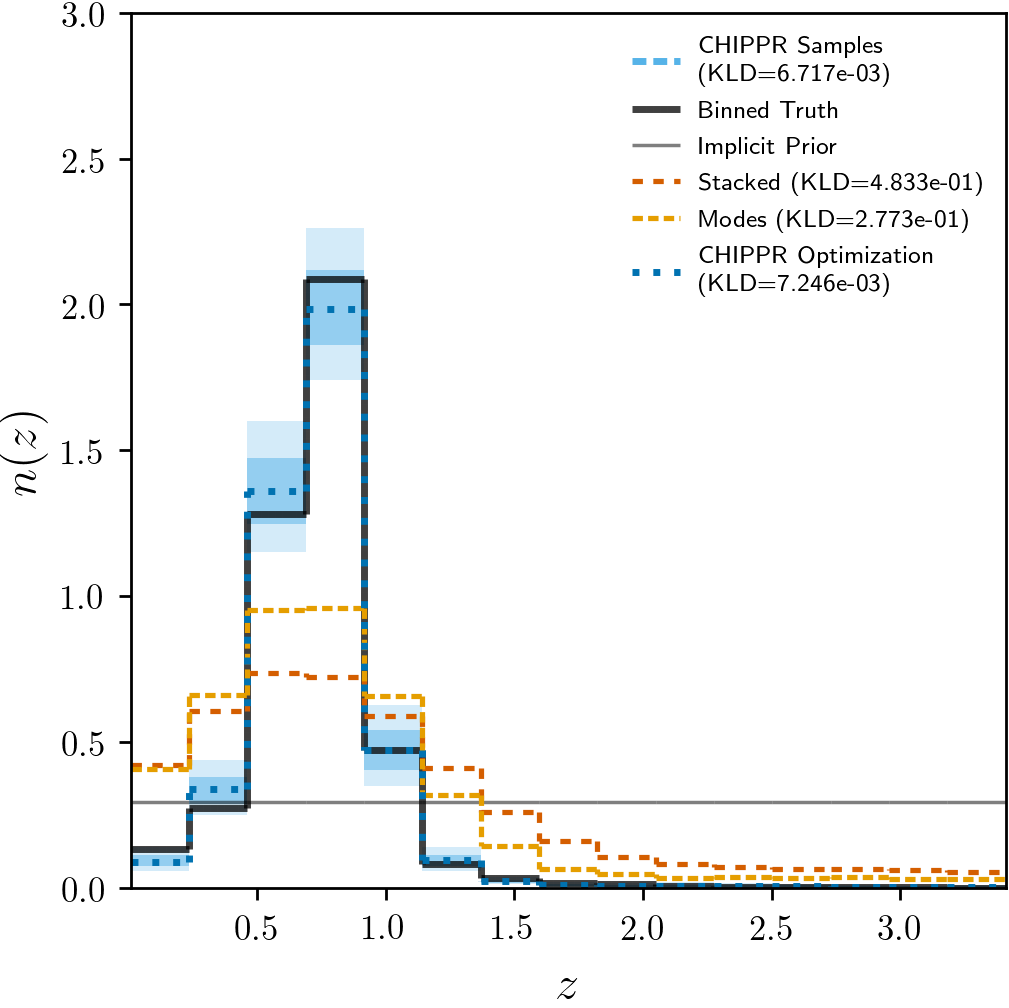
\includegraphics[width=0.24\textwidth]{figures/chippr/2single_lsst_lin_estimators.png}
		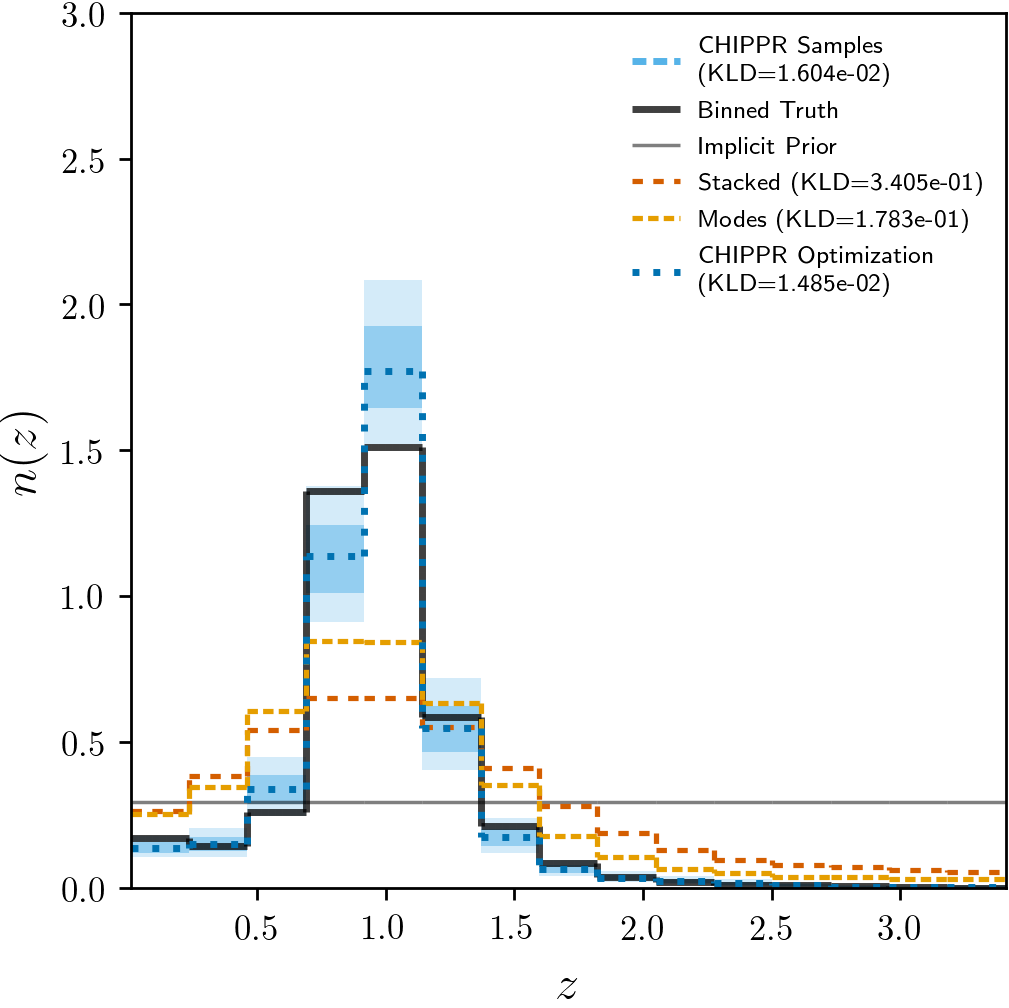
\includegraphics[width=0.24\textwidth]{figures/chippr/3single_lsst_lin_estimators.png}
		\caption{The \chippr-derived and other estimators of \nz\ in each tomographic bin.
		\aim{Make this one big plot instead of four little ones to eliminate repeated axis labels and legend.}}
		\figlabel{fig:per-bin-ests}
	\end{center}
\end{figure*}

I then used the different estimators of \nz\ in a cosmological forecasting procedure with \cosmolike.
\aim{Cite Krause here.}

\begin{figure*}
	\begin{center}
		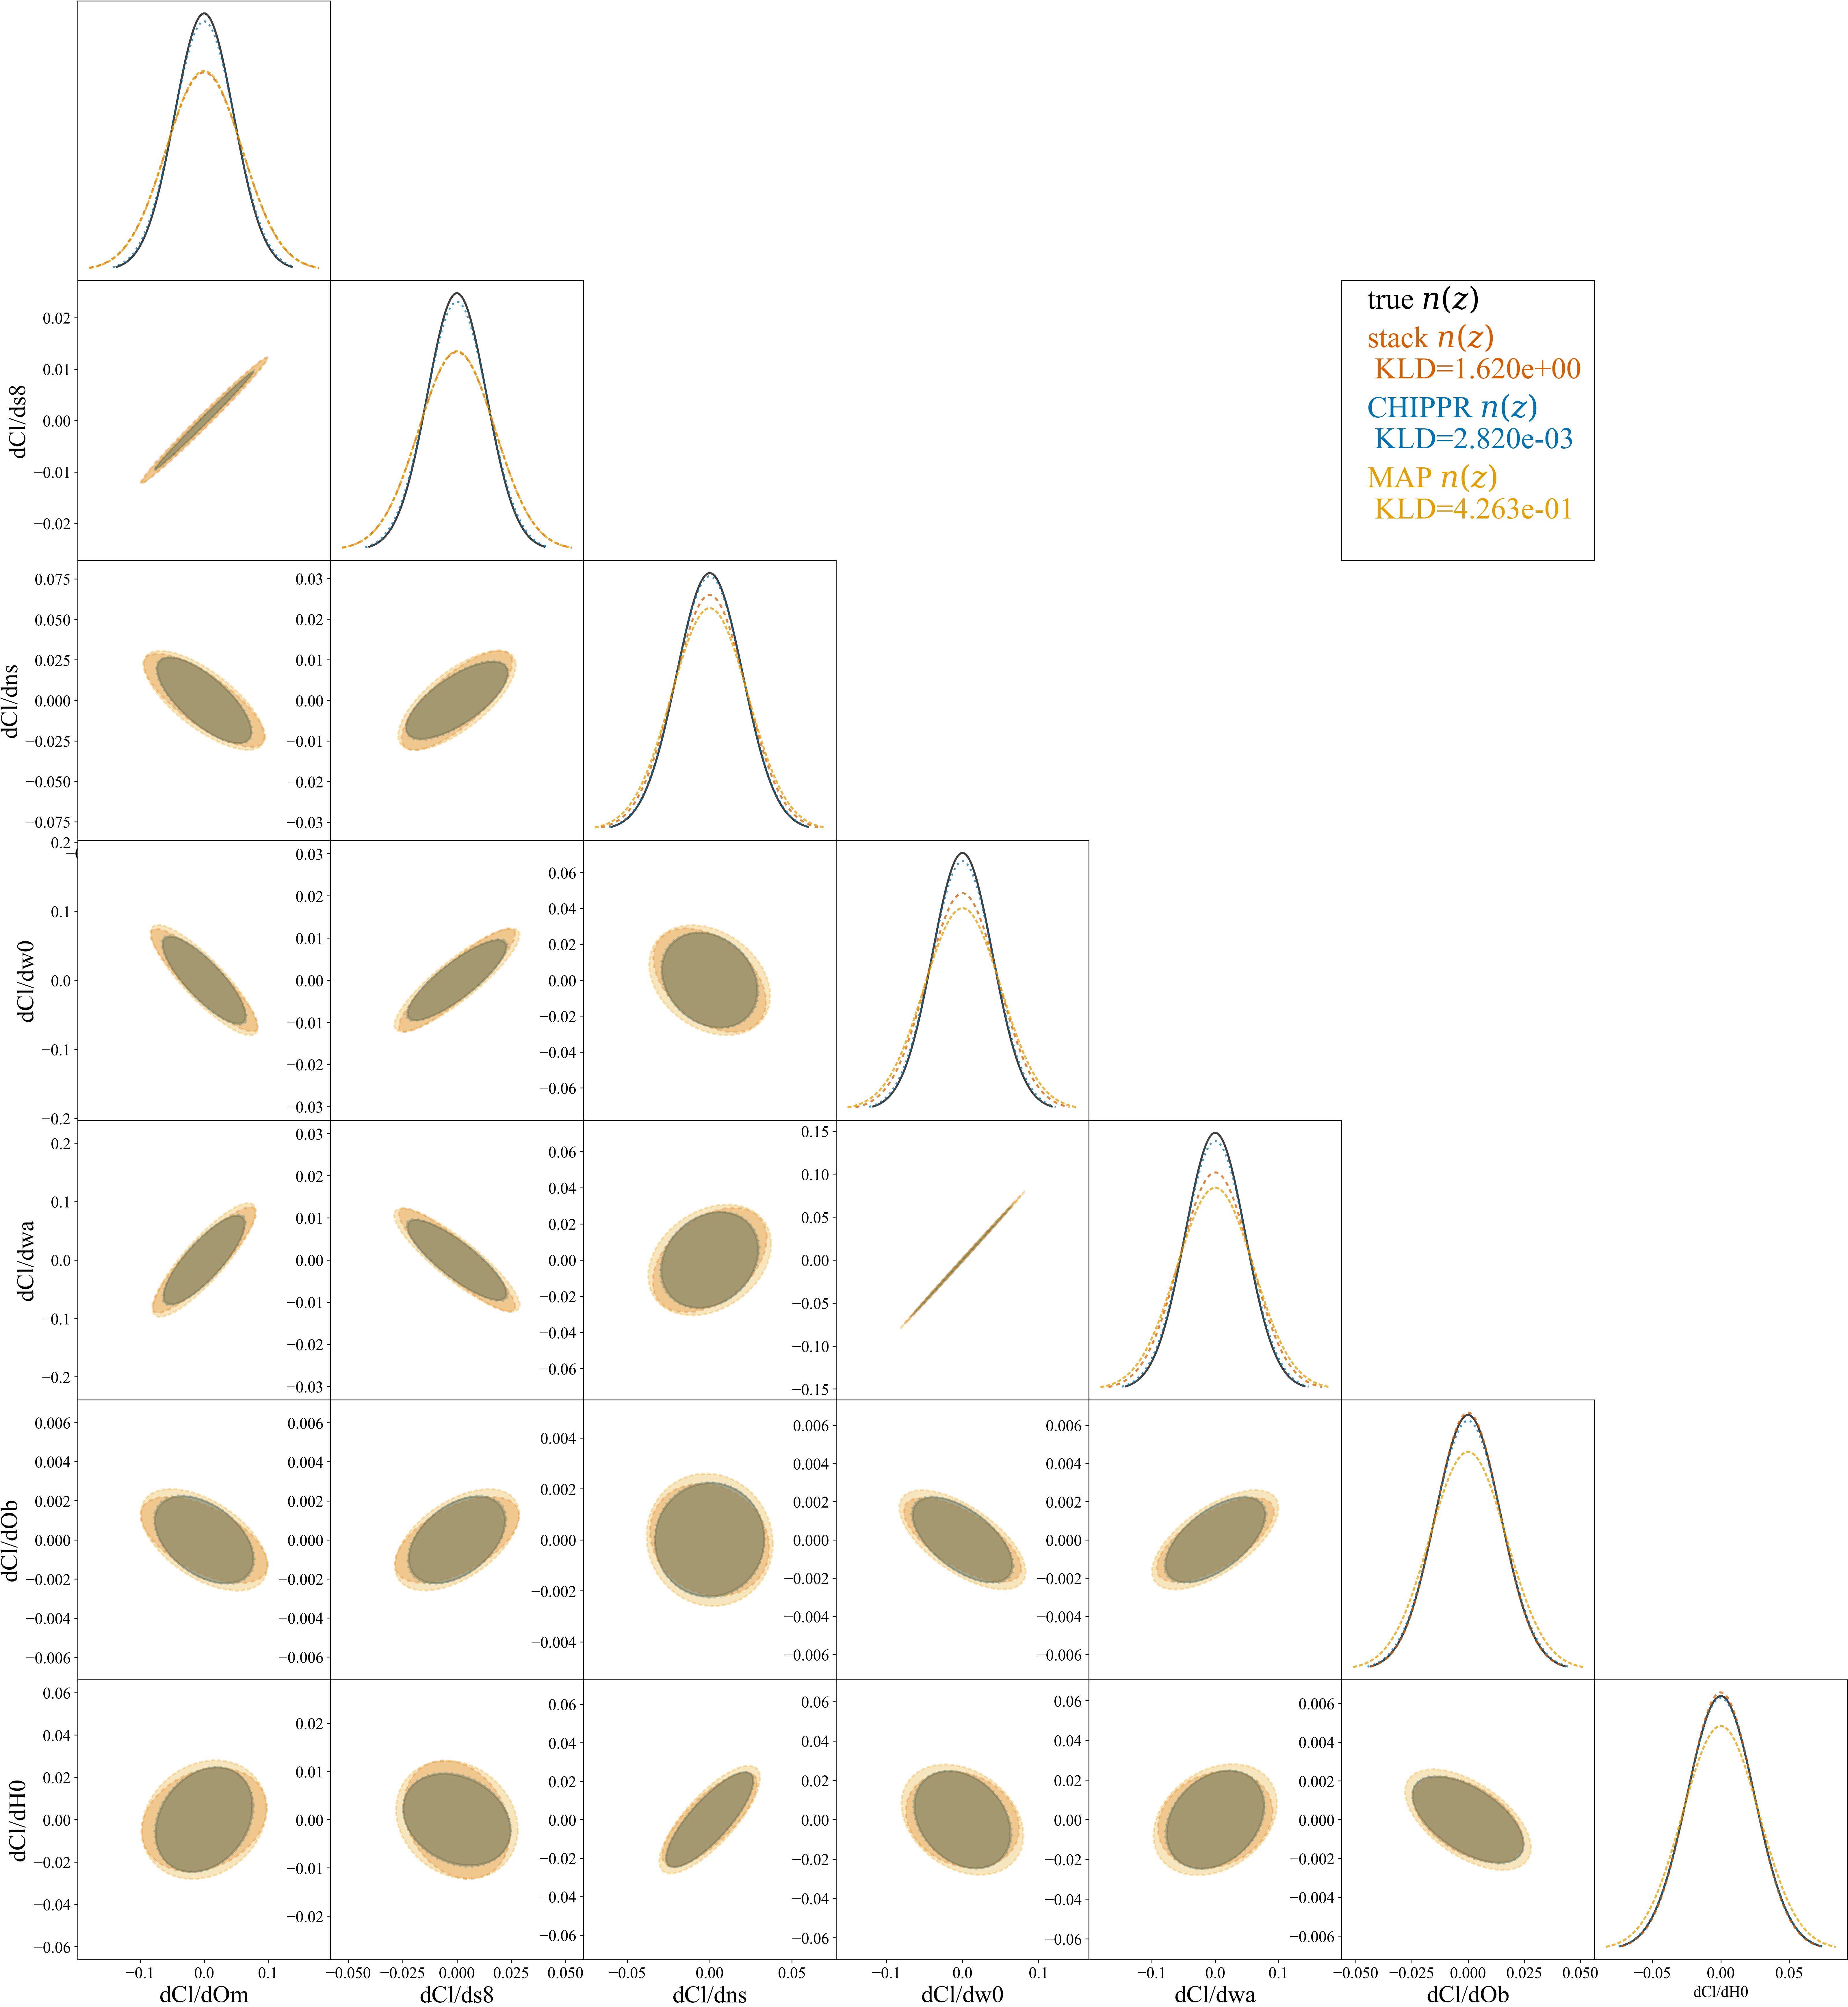
\includegraphics[width=0.99\textwidth]{figures/chippr/final_plot.png}
		\caption{The result of propagating the estimators of \nz\ of \Fig{fig:per-bin-ests} to a subset of cosmological parameters.}
		\figlabel{fig:cornerplot}
	\end{center}
\end{figure*}


\aim{Discuss these results here!}

\aim{Hogg says ``I think it would be good to talk a little quantitatively about where people need to know N(z) and other one-point statistics, and how much they will get various things wrong if they don't know these correctly. 
	And situate that discussion within the current context of cosmological parameter estimation and precision cosmology.''}

\aim{Caveats: I don't believe in tomographic binning because it's non-physical, and we won't have the true redshifts so there will be additional errors if tomography is used.}

\subsection{Violations of the model}
\sectlabel{sec:violations}

In these tests, the \pzip s are made to the \lsst\ requirements but the implicit prior used for the inference is not the same as the implicit prior used for generating the data.

\begin{figure*}
	\begin{center}
		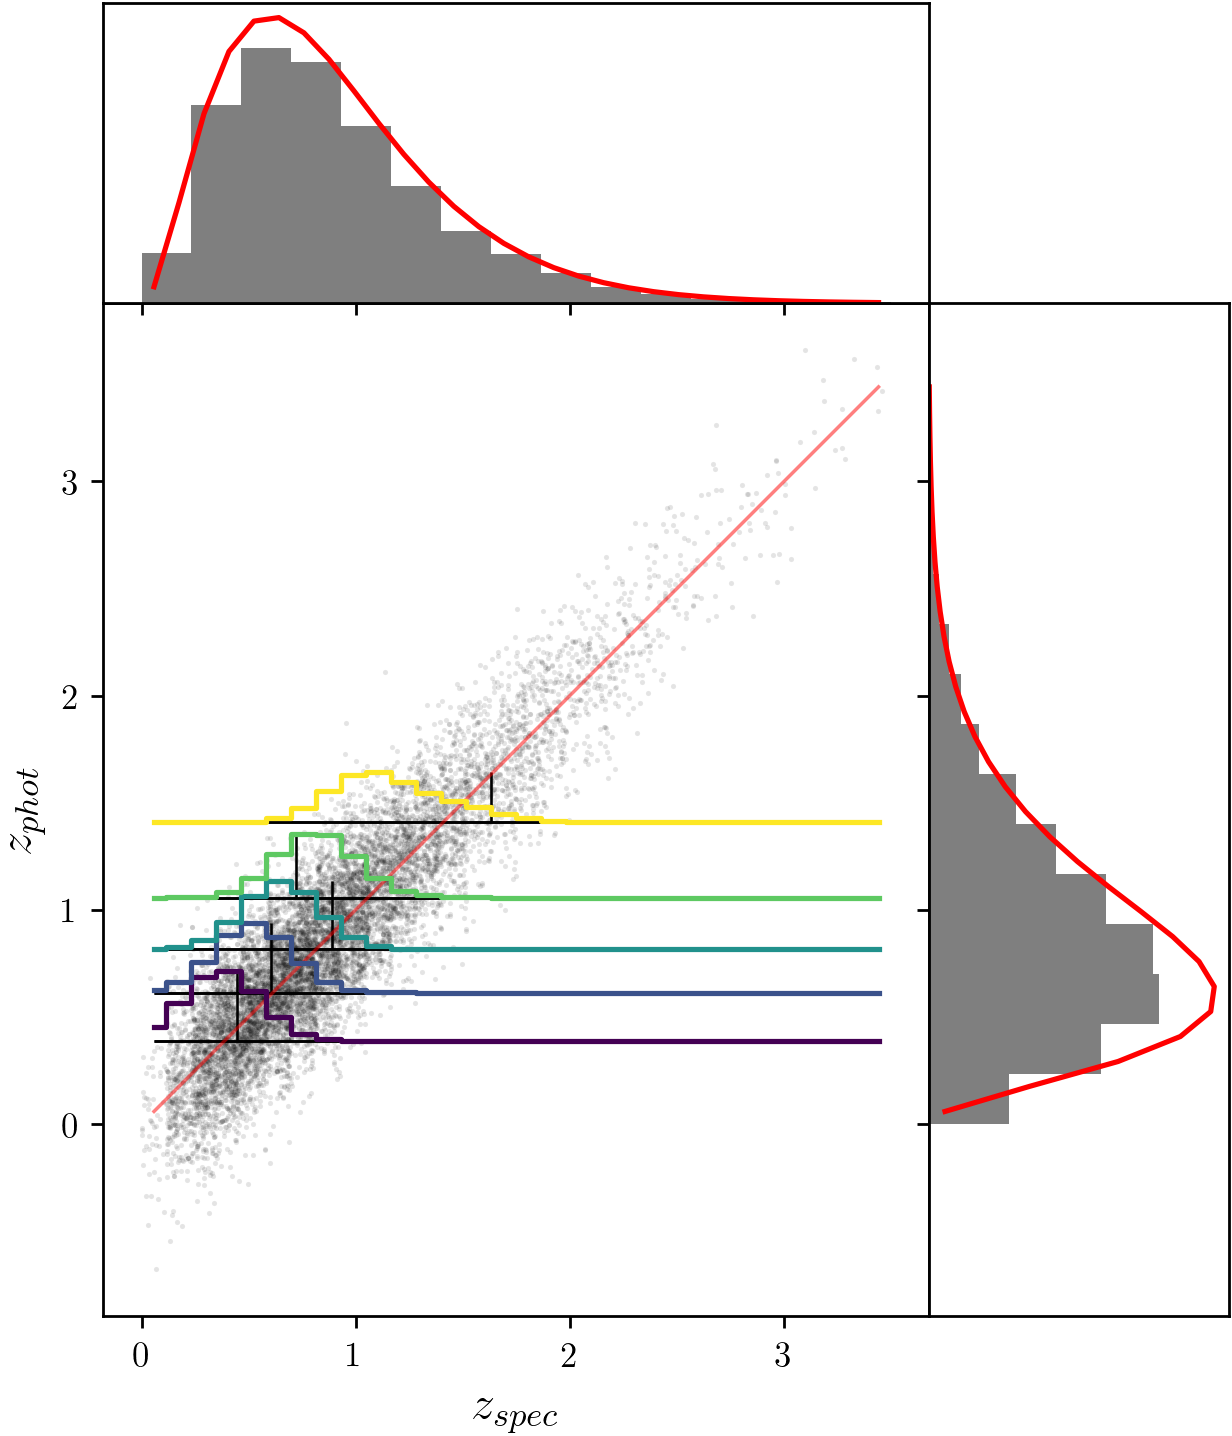
\includegraphics[width=0.45\textwidth]{figures/chippr/wrong_scatter.png}
		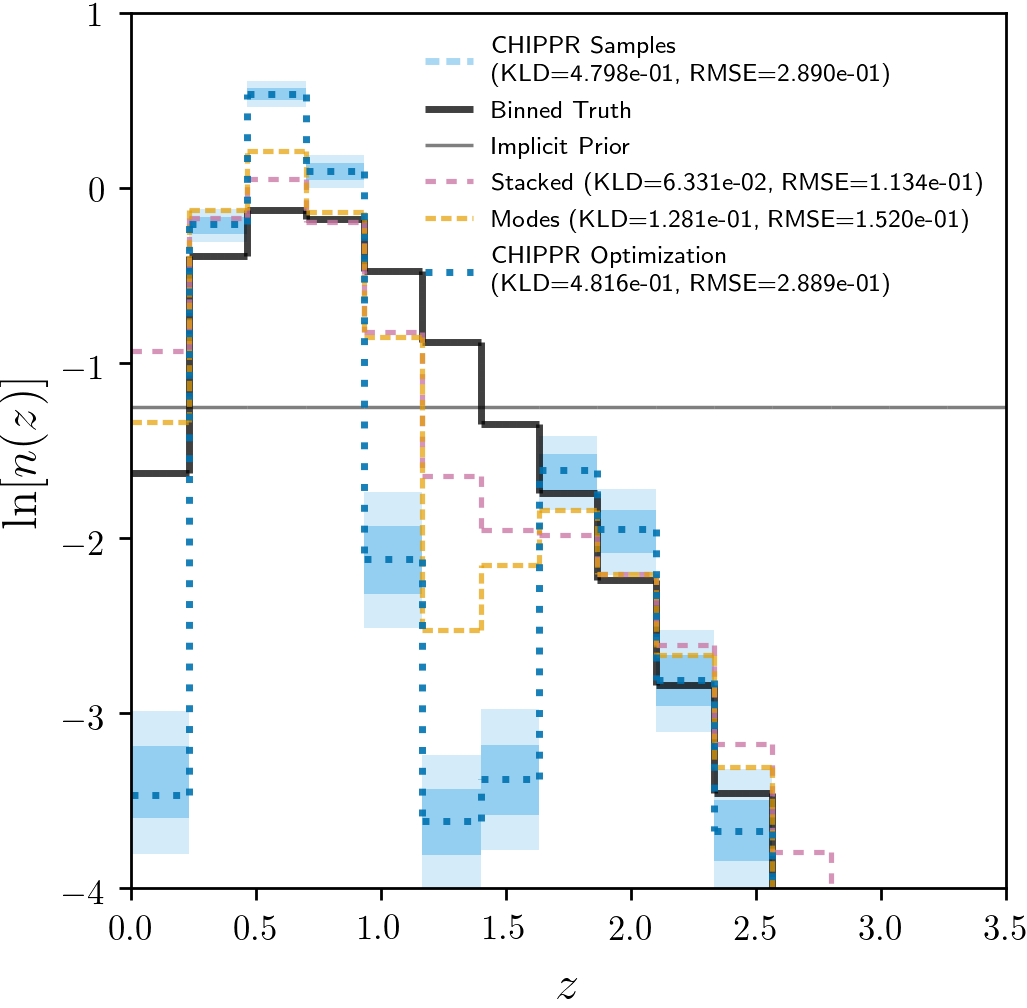
\includegraphics[width=0.45\textwidth]{figures/chippr/wrong_log_estimators.png}
		\caption{\aim{Update the figures for this to use the same conditions as \Sect{sec:lsstdemo} but one of the implicit priors from \Sect{sec:interim} for generating the data and the other for the inference.}}
		\figlabel{fig:mischaracterized}
	\end{center}
\end{figure*}

%\subsection{Real Data}
%\sectlabel{sec:boss}
%
%\aim{Commented out but may add back in later.}

%We also test this method on subsets of the published \pzpdf s of \sdss\ III DR 10. 
%A sampling of the provided interim photo-$z$ posteriors of dimension $K=35$ for $z_{min}=0.3$ and $z_{max}=1.4$ is shown in the top panel of \Fig{fig:datapzs}.  
%
%All tests in this paper will be conducted with $z_{0}=0.0$, $z_{K}=1.1$, and $K=35$, the endpoints and dimensionality of the published BOSS DR8 photo-$z$ interim posteriors \citet{Sheldon2012}.  
%We also define $\bar{z}_{k}\equiv(z_{k}+z_{k-1})/2$.
%The brightest half of this pseudo-random sampling are selected for another test, with photo-$z$ interim posterior samples shown in the bottom panel of \Fig{fig:datapzs}.  
%The interim prior used for this set of interim photo-$z$ posteriors is the reweighted estimator of $N(z)$ of \citet{Sheldon2012}.  
%In these cases the true $N(z)$ is not known, but the fully probabilistic method presented here may still be compared to what is obtained by alternative approaches.
%
%\begin{figure}
%	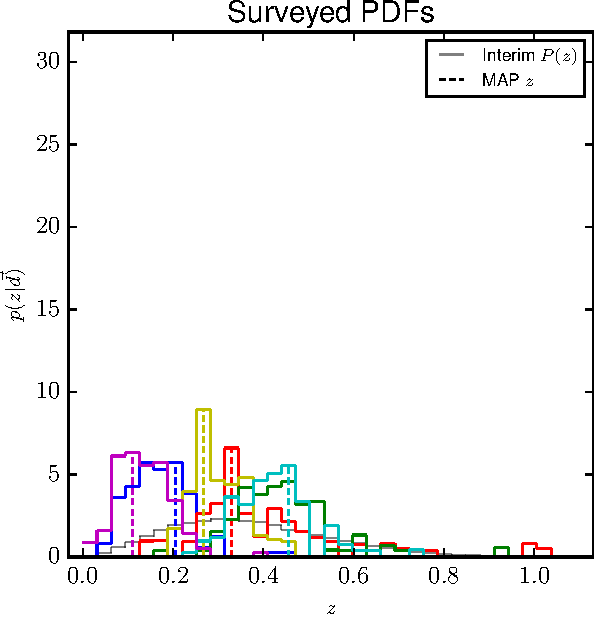
\includegraphics[width=0.5\textwidth]{figures/chippr/boss_samplepzs.pdf}\\
%	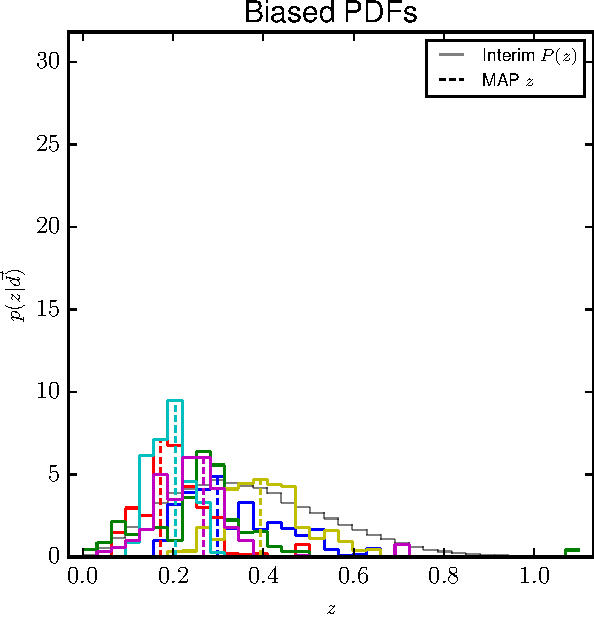
\includegraphics[width=0.5\textwidth]{figures/chippr/bias_samplepzs.pdf}
%	\caption{Same as \Fig{fig:nullpzs} but for real data.  
%		A pseudo-random sampling of BOSS DR 10 photo-$z$ posteriors produced by \citet{Sheldon2012} (top panel) are clearly much noisier than those of the fiducial case.  
%		A random sampling of the brightest half of the pseudo-random BOSS DR10 sample (bottom panel) corresponds to much cleaner photo-$z$ posteriors.}
%	\figlabel{fig:datapzs}
%\end{figure}

%The results of the inference of the redshift distribution function from a pseudo-random sample of BOSS DR10 data described in \Sect{sec:data} are shown in \Fig{fig:dataparam} and \Fig{fig:datacomp}.  
%
%The most striking feature of \Fig{fig:dataparam} aside from the stark difference between the mean of the samples and the interim prior is the major systematic in the samples from the posterior distribution is observed at high redshift.  
%Because the data itself exhibits high uncertainty at high $z$ in the form of local maxima of the photo-$z$ interim posteriors, a reflection of the inherent degeneracies that give rise to catastrophic photo-$z$ errors, it is natural that there be large errors in that region.  
%
%\begin{figure}
%	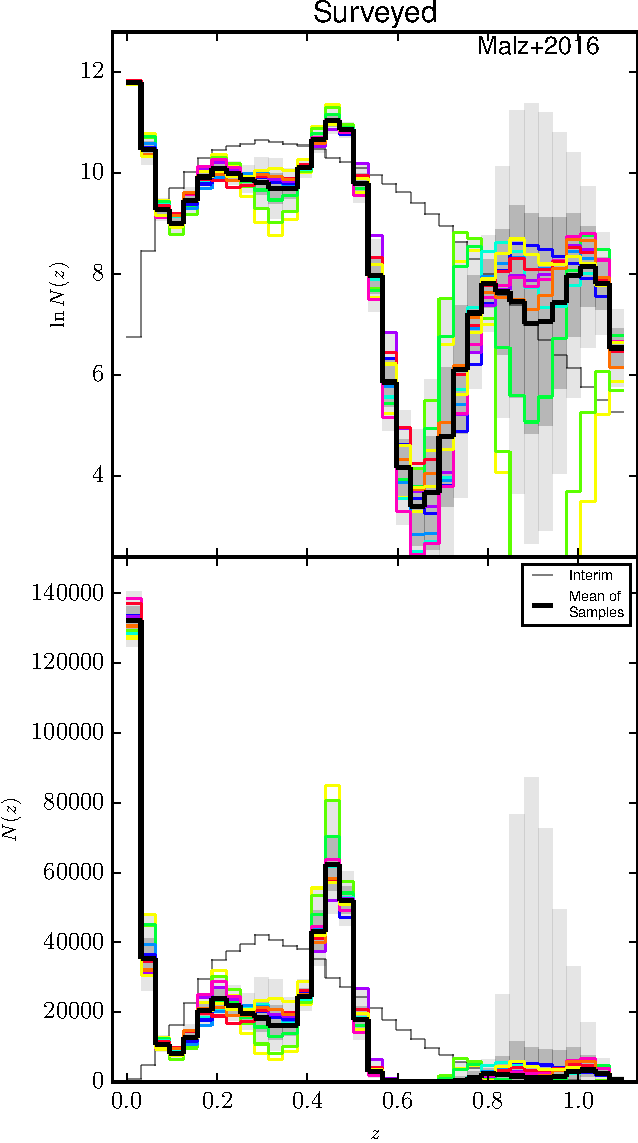
\includegraphics[width=0.5\textwidth]{figures/chippr/boss_samps.pdf}
%	\caption{Samples from the full posterior (colored lines) of the subsample differ substantially from the interim prior (gray).  
%		The mean of samples (thick, black line) and associated error bars ($1\sigma$ in dark gray, $2\sigma$ in light gray) are in line with the sampled values.}
%	\figlabel{fig:dataparam}
%\end{figure}
%
%\Fig{fig:datacomp} also shows the broader error bars in a small region of high redshift, but it has the additional information of how other estimators perform.  
%The results of stacking and reduction of interim photo-$z$ posteriors to point estimators are strongly biased toward the interim prior, especially stacking.  
%Given that stacking has been validated by the results' similarity to the interim prior, it is especially grave that it trivially reproduce it; if the interim prior is inappropriate, stacking is guaranteed to fail because it do not account for the effect of the interim prior on the interim photo-$z$ posteriors, permitting it to dominate over the underling likelihoods.  
%The result of marginalized maximum likelihood estimation is also shown to be numerically unstable, a possible effect of the extreme multimodality of the data.  
%
%\begin{figure}
%	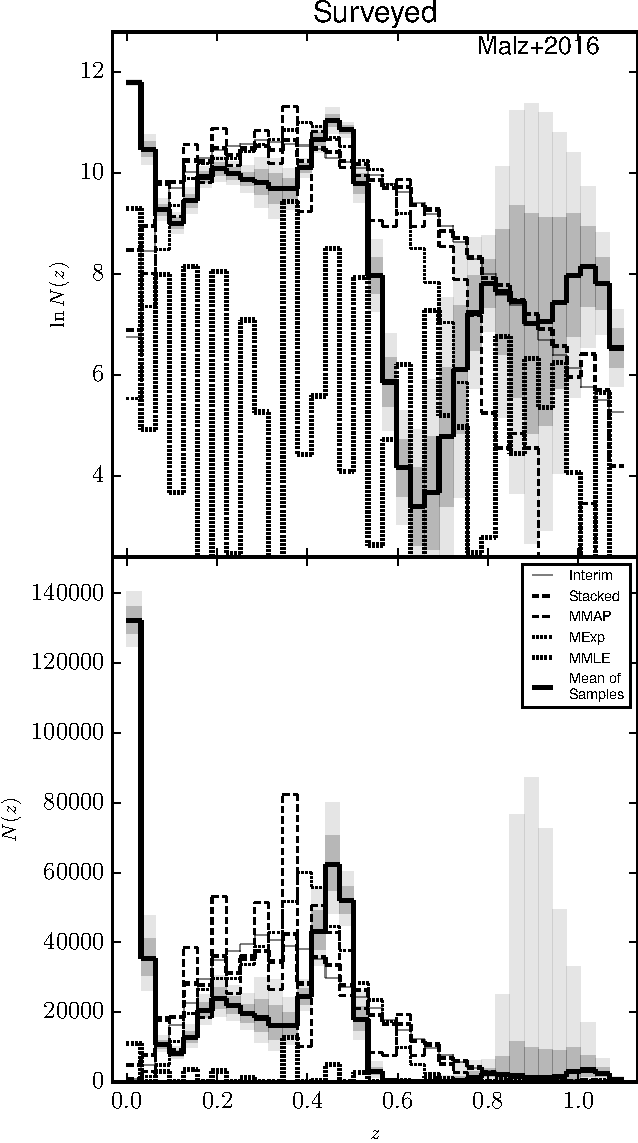
\includegraphics[width=0.5\textwidth]{figures/chippr/boss_comps.pdf}
%	\caption{It can be seen that the stacked estimator (thick, dashed line) almost perfectly reproduces the interim prior (gray line), while the marginalized maximum a posteriori estimator (thin, dashed line) and marginalized expected value estimator (thin, dotted line) do so with some instability.  
%		The marginalized maximum likelihood estimator (thick, dotted line) is most unstable, while the mean of the posterior samples (thick, solid line) predicts a very different redshift distribution function than the interim prior, with a peculiar feature in the error bars ($1\sigma$ in dark gray, $2\sigma$ in light gray) at high redshift.}
%	\figlabel{fig:datacomp}
%\end{figure}
%
%The BOSS subsample is further subsampled by imposing a cut in $r$-band magnitude (at the median magnitude) to approximate the behavior of a heavily biased galaxy survey with a magnitude limit.  
%This is motivated by the question of what data is behind the feature in the posterior distribution's error bars at high redshift.  
%Recall that samples of photo-$z$ interim posteriors are shown in the lower panel of \Fig{fig:datapzs}.  
%The results of the inference are shown in \Fig{fig:biasparam} and \Fig{fig:biascomp}.  
%
%\begin{figure}
%	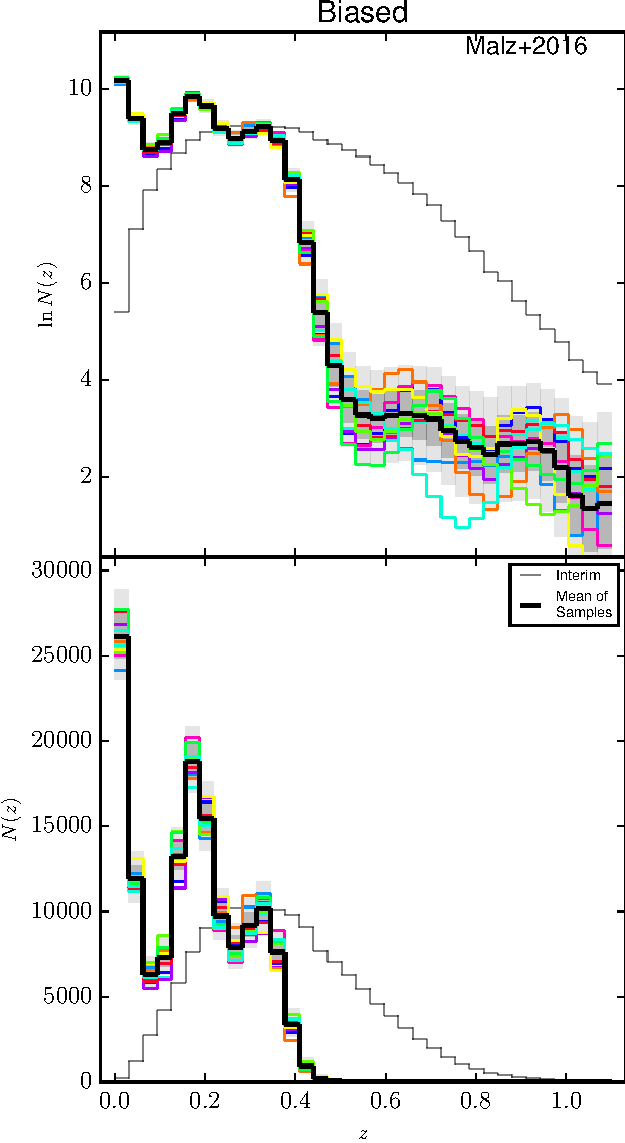
\includegraphics[width=0.5\textwidth]{figures/chippr/bias_samps.pdf}
%	\caption{Samples from the full posterior (colored lines) of the biased subsample still differ substantially from the interim prior (gray).  
%		The mean of samples (thick, black line) and associated error bars ($1\sigma$ in dark gray, $2\sigma$ in light gray) are in line with the sampled values.}
%	\figlabel{fig:biasparam}
%\end{figure}
%
%\begin{figure}
%	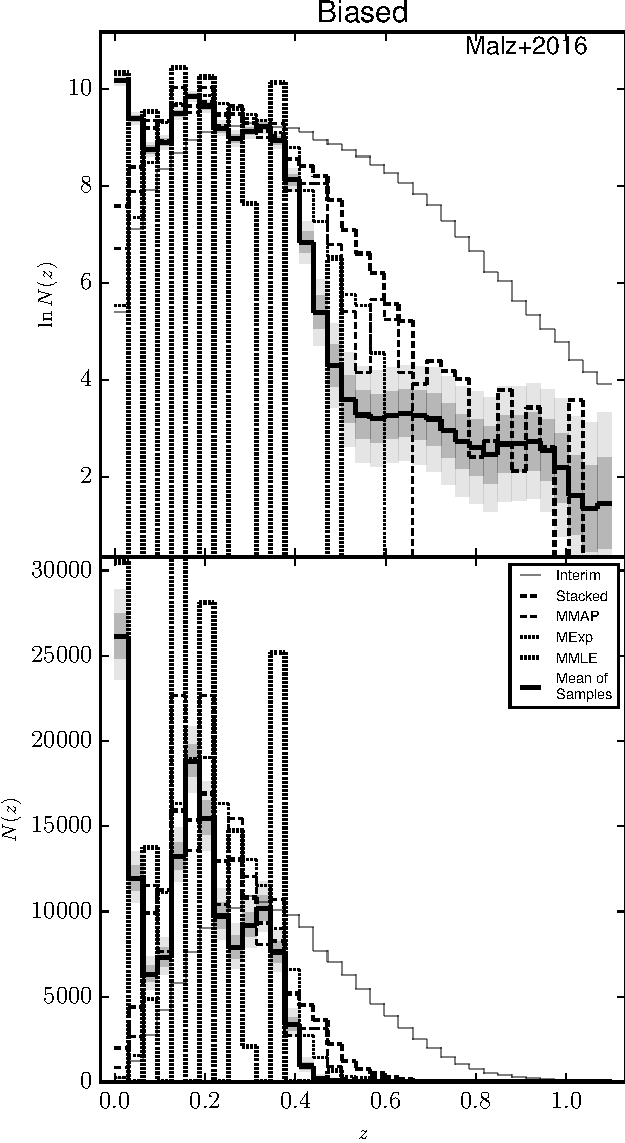
\includegraphics[width=0.5\textwidth]{figures/chippr/bias_comps.pdf}
%	\caption{The mean of posterior samples (thick, solid line) differs from the interim prior (gray line) more than the alternative estimators, exhibiting some features at low redshift.  
%		It can be seen that the stacked estimator (thick, dashed line) is most biased towards the interim prior, though the effect is also seen in the marginalized maximum a posteriori estimator (thin, dashed line) and marginalized expectation value estimator (thin, dotted line).  
%		The marginalized MLE (thick, dotted line) is still highly unstable.  
%		The error bars ($1\sigma$ in dark gray, $2\sigma$ in light gray) do not exhibit the same behavior as in the unbiased subsample.}
%	\figlabel{fig:biascomp}
%\end{figure}
%
%There are two notable differences between the unbiased and biased subsamples of the BOSS DR10 pseudo-random subsample.  
%First, the stacked and point estimators are less biased toward the interim prior.  
%This may be due to the way the interim prior was chosen, such that it was influenced strongly by the dimmest galaxies.  
%Second, the high-redshift feature in the error bars is not present once a magnitude cut is imposed.  
%From this one can conclude that the signal and associated error bars in that region were caused by the sampler's assignment high redshifts to poorly constrained interim photo-$z$ posteriors corresponding to the dimmest galaxies. 

\section{Conclusion}
\sectlabel{sec:con}

\aim{I still need to update the language in this section for consistency with the rest of \Chap{chippr}.}

This study derives and demonstrates a mathematically consistent implementation of inference of a one-point statistic based on any existing catalog of \pzpdf s.  
The fully Bayesian method, based in the fundamental laws of probability, begins with a graphical model corresponding to equations for the full posterior.  
The technique developed in this paper is applied to the example of the redshift density function \nz\ with promising results on mock data; not only is this the only mathematically correct approach to the problem, it also recovers the true parameter values better than popular alternatives.  

In the tests on simulated data performed here, the full posterior distribution over the hyperparameters defining $N(z)$ derived by this method is consistent with the true redshift distribution function, making the mean of sampled values an excellent point estimator of $N(z)$.  
The information contained in the full posterior distribution's shape convey the traditional error bar information without having to explicitly propagate any error estimates.  
\aim{Refer to quantitative results on KLD of \Nz\ and cosmological parameter space.}
%The results of those tests is summarized below and in \Tab{tab:kld}, where lower values indicate a closer match between the true $N(z)$ and the estimator.  
%Tests were also performed on subsets of BOSS DR10 data with results consistent with those of simulations.

The following conclusions and recommendations can be made with confidence:

\begin{enumerate}
	\item Both the marginalized maximum likelihood estimator and the mean of the samples are good point estimators of the redshift distribution function; the error bars on the posterior distribution over hyperparameters are generally reliable and easier to derive than error bars from traditional point estimators of the redshift distribution function.
	\item Even in the case of precise data, traditional methods fail, and they do even worse with imprecise data; the error bars of the mean of posterior samples, however, are accurate.  When data quality worsens with redshift, all estimators are affected, but the inaccuracy is quantified by the full distribution of the posterior samples whereas the alternative estimators require separate error propagation.  
	\item When data suffers from inaccuracies, as in the case of multimodal interim photo-$z$ posteriors, the marginalized maximum likelihood estimator performs comparably to the mean of the posterior samples
	\item The marginalized maximum likelihood estimator is an excellent estimator for strongly featured redshift distribution function with simple, clean photo-$z$ posteriors; stacking smooths features more than sampling and photo-$z$ point estimation.
	\item When the interim prior is known to be a poor approximation to the data, only the marginalized MLE and mean of sampled values are satisfactory estimators of the redshift distribution function because they are the only methods that can account for the bias introduced into the photo-$z$ posteriors; this is the most compelling case for the sampler because of the ubiquity of inappropriate interim priors.
\end{enumerate}

By showing that this method is effective in recovering the true redshift distribution function and posterior distributions on its parameters from catalogs of \pzpdf s, this work supports the production of \pzpdf s by upcoming photometric surveys such as \lsst\ so that more accurate inference of physical parameters may be accessible to the scientific community.  
We discourage researchers from co-adding \pzpdf s or converting them into point estimates of redshift and instead recommend the use of Bayesian probability to guide the usage of \pzpdf s in science.  
We emphasize to those who produce \pzpdf s from data that it is essential to release the implicit prior used in generating this data product in order for proper inference to be conducted by consumers of this information.

The technique herein developed is applicable with minimal modification to other one-point statistics of redshift to which we will apply this method in the future, such as the redshift-dependent luminosity function and weak lensing mean distance ratio.  
Future work will also include the extension of this fully probabilistic approach to higher-order statistics of redshift such as the two-point correlation function.

\section*{Chapter acknowledgements}

I thank Elisabeth Krause for assistance with the \texttt{CosmoLike} code, Mohammadjavad Vakili for statistical insights, Geoffrey Ryan for programming advice, and Boris Leistedt for other helpful comments in the development of \Chippr.
